% ============================================================================
%  Doc P -- SPEAR3 RF System: RF Physics, Control Theory and Physical Plant
%  Build:  powershell -ExecutionPolicy Bypass -File build.ps1 -Doc P
%  Engine: LuaLaTeX (required -- see the Unicode note in preamble.tex)
% ============================================================================
\documentclass[letterpaper,11pt]{article}
% ============================================================================
%  SPEAR3 RF System documentation -- shared preamble
%  Engine: LuaLaTeX.  Build with build.ps1 (latexmk -lualatex).
% ============================================================================

\usepackage[letterpaper,top=1in,bottom=1in,left=1.05in,right=1.05in]{geometry}

% --- fonts -----------------------------------------------------------------
\usepackage{fontspec}
\setmainfont{TeX Gyre Termes}
\setsansfont{TeX Gyre Heros}
\setmonofont{Consolas}[Scale=0.86]

% --- Unicode safety --------------------------------------------------------
% LuaLaTeX DROPS unmapped glyphs SILENTLY -- an unmapped U+03BC turns "8 uF"
% into "8 F".  Every non-ASCII character used in these documents is mapped
% here.  The build script fails if the log reports "Missing character".
\usepackage{newunicodechar}
\newunicodechar{μ}{\ensuremath{\mu}}      \newunicodechar{µ}{\ensuremath{\mu}}
\newunicodechar{Ω}{\ensuremath{\Omega}}   \newunicodechar{≈}{\ensuremath{\approx}}
\newunicodechar{≥}{\ensuremath{\geq}}     \newunicodechar{≤}{\ensuremath{\leq}}
\newunicodechar{≠}{\ensuremath{\neq}}     \newunicodechar{×}{\ensuremath{\times}}
\newunicodechar{÷}{\ensuremath{\div}}     \newunicodechar{±}{\ensuremath{\pm}}
\newunicodechar{−}{\ensuremath{-}}        \newunicodechar{√}{\ensuremath{\sqrt{}}}
\newunicodechar{α}{\ensuremath{\alpha}}   \newunicodechar{β}{\ensuremath{\beta}}
\newunicodechar{φ}{\ensuremath{\varphi}}  \newunicodechar{ω}{\ensuremath{\omega}}
\newunicodechar{Δ}{\ensuremath{\Delta}}   \newunicodechar{τ}{\ensuremath{\tau}}
\newunicodechar{θ}{\ensuremath{\theta}}   \newunicodechar{λ}{\ensuremath{\lambda}}
\newunicodechar{π}{\ensuremath{\pi}}      \newunicodechar{σ}{\ensuremath{\sigma}}
\newunicodechar{₀}{\ensuremath{_0}}       \newunicodechar{₁}{\ensuremath{_1}}
\newunicodechar{₂}{\ensuremath{_2}}       \newunicodechar{²}{\ensuremath{^2}}
\newunicodechar{³}{\ensuremath{^3}}       \newunicodechar{⁴}{\ensuremath{^4}}
\newunicodechar{⁻}{\ensuremath{^-}}       \newunicodechar{⁺}{\ensuremath{^+}}
\newunicodechar{→}{\ensuremath{\rightarrow}}
\newunicodechar{←}{\ensuremath{\leftarrow}}
\newunicodechar{↔}{\ensuremath{\leftrightarrow}}
\newunicodechar{⇒}{\ensuremath{\Rightarrow}}
\newunicodechar{⊕}{\ensuremath{\oplus}}   \newunicodechar{∥}{\ensuremath{\parallel}}
\newunicodechar{°}{\ensuremath{^\circ}}   \newunicodechar{·}{\ensuremath{\cdot}}
\newunicodechar{≪}{\ensuremath{\ll}}      \newunicodechar{≫}{\ensuremath{\gg}}
\newunicodechar{✓}{\checkmark}            \newunicodechar{⚠}{\textbf{!}}
\newunicodechar{–}{--}                    \newunicodechar{—}{---}

% --- maths and units -------------------------------------------------------
\usepackage{amsmath,amssymb}
\usepackage{siunitx}
\DeclareSIUnit\voltampere{VA}
\DeclareSIUnit\VAR{var}
% range-phrase must not rely on literal spaces (LaTeX strips them from a key
% value, so "{ to }" renders as "10to20") and must force text mode (siunitx
% sets numbers in math, where a bare "--" becomes two minus signs).
\sisetup{per-mode=symbol,range-phrase={\text{--}},range-units=single,
         group-minimum-digits=4,detect-weight=true}

% --- tables ----------------------------------------------------------------
\usepackage{longtable,booktabs,array,tabularx,multirow}
\usepackage{ragged2e}
\setlength{\LTleft}{0pt}\setlength{\LTright}{0pt}
\renewcommand{\arraystretch}{1.18}
% left-aligned, hyphenating paragraph column used by every wide table
\newcolumntype{P}[1]{>{\RaggedRight\arraybackslash}p{#1}}
% Same, but \small: for dense tables.  The size must live in the column type --
% wrapping a longtable in {\small ...} breaks its page-breaking \write.
\newcolumntype{Q}[1]{>{\small\RaggedRight\arraybackslash}p{#1}}

% --- graphics and figures --------------------------------------------------
\usepackage{graphicx}
% Resolved from the document's own folder, which is the working directory.
\graphicspath{{../common/}{../common/photos/}{../common/generated/}}
\usepackage{float}
\usepackage[font=small,labelfont=bf,width=0.92\linewidth]{caption}
\usepackage{comment}

% A figure must not drift out of the section it belongs to.  With 47 floats
% LaTeX will otherwise push them pages away from the text that discusses them.
\usepackage[section]{placeins}

% Default float parameters are tuned for papers with two or three figures.
% This document is figure-dense, so allow more of a page to be float and more
% floats per page; without this, figures queue up and drift several pages.
\renewcommand{\topfraction}{0.88}
\renewcommand{\bottomfraction}{0.70}
\renewcommand{\textfraction}{0.10}
\renewcommand{\floatpagefraction}{0.72}
\setcounter{topnumber}{3}
\setcounter{bottomnumber}{2}
\setcounter{totalnumber}{5}

% Image size policy.  Photographs are capped in BOTH width and height so that
% no figure can ever exceed roughly half a page, whatever its aspect ratio.
\newlength{\photomaxh}\setlength{\photomaxh}{0.34\textheight} % ~1/3 page
\newlength{\widemaxh} \setlength{\widemaxh}{0.46\textheight}  % ~1/2 page

% \photofig{file}{caption}{label}      -- default, about 1/3 page
\newcommand{\photofig}[3]{%
  \begin{figure}[htbp]\centering
    \includegraphics[width=0.62\linewidth,height=\photomaxh,keepaspectratio]{#1}%
    \caption{#2}\label{#3}
  \end{figure}}
% \widefig{file}{caption}{label}       -- for detailed schematics, about 1/2 page
\newcommand{\widefig}[3]{%
  \begin{figure}[htbp]\centering
    \includegraphics[width=0.94\linewidth,height=\widemaxh,keepaspectratio]{#1}%
    \caption{#2}\label{#3}
  \end{figure}}
% \smallfig{file}{caption}{label}      -- for low-resolution sources
\newcommand{\smallfig}[3]{%
  \begin{figure}[htbp]\centering
    \includegraphics[width=0.44\linewidth,height=0.26\textheight,keepaspectratio]{#1}%
    \caption{#2}\label{#3}
  \end{figure}}
% \tallfig{file}{caption}{label}       -- portrait-orientation photographs.
% A tall photo capped at \photomaxh comes out only ~45 mm wide, so these are
% capped by height instead and allowed a narrower column.
\newcommand{\tallfig}[3]{%
  \begin{figure}[tbp]\centering
    \includegraphics[width=0.46\linewidth,height=0.50\textheight,keepaspectratio]{#1}%
    \caption{#2}\label{#3}
  \end{figure}}
% two portrait photographs side by side under one caption:
% \tallpairfig{fileA}{subA}{labA}{fileB}{subB}{labB}{caption}{label}
\newcommand{\tallpairfig}[8]{%
  \begin{figure}[tbp]\centering
    \begin{minipage}[b]{0.46\linewidth}\centering
      \includegraphics[width=\linewidth,height=0.40\textheight,keepaspectratio]{#1}%
      \subcaption{#2}\label{#3}
    \end{minipage}\hfill
    \begin{minipage}[b]{0.46\linewidth}\centering
      \includegraphics[width=\linewidth,height=0.40\textheight,keepaspectratio]{#4}%
      \subcaption{#5}\label{#6}
    \end{minipage}
    \caption{#7}\label{#8}
  \end{figure}}
% two photographs side by side, each about 1/4 page
\newcommand{\pairfig}[6]{%
  \begin{figure}[htbp]\centering
    \begin{minipage}[t]{0.48\linewidth}\centering
      \includegraphics[width=\linewidth,height=0.26\textheight,keepaspectratio]{#1}%
      \subcaption{#2}\label{#3}
    \end{minipage}\hfill
    \begin{minipage}[t]{0.48\linewidth}\centering
      \includegraphics[width=\linewidth,height=0.26\textheight,keepaspectratio]{#4}%
      \subcaption{#5}\label{#6}
    \end{minipage}
  \end{figure}}
\usepackage{subcaption}

% --- diagrams --------------------------------------------------------------
\usepackage{tikz}
\usetikzlibrary{arrows.meta,positioning,fit,backgrounds,calc,shapes.geometric,
                shapes.misc,chains,decorations.pathreplacing,patterns,matrix}
\usepackage{pgfplots}\pgfplotsset{compat=1.18}
\usepackage{rotating}                  % sidewaysfigure, if a portrait page is wanted
\usepackage{pdflscape}                 % landscape: rotates the PAGE in the PDF
\usepackage[export]{adjustbox}         % max width= / max height= on a box

% Shrink a diagram to the text width only if it would otherwise overflow, so
% figures drawn at their natural scale are never enlarged or needlessly shrunk.
\newsavebox{\fitbox}
\newenvironment{fitpicture}
  {\begin{lrbox}{\fitbox}}
  {\end{lrbox}%
   \ifdim\wd\fitbox>\linewidth
     \resizebox{\linewidth}{!}{\usebox{\fitbox}}%
   \else
     \usebox{\fitbox}%
   \fi}

% House diagram style.  Keep every block diagram in these styles so the
% document reads as one drawing set rather than a scrapbook.
\definecolor{cCtrl}{HTML}{1F4E79}   % control / EPICS
\definecolor{cPlc} {HTML}{7F6000}   % PLC / interlock
\definecolor{cPwr} {HTML}{843C0C}   % high power
\definecolor{cRf}  {HTML}{2E6B34}   % RF signal path
\definecolor{cNeut}{HTML}{3B3B3B}
\tikzset{
  blk/.style   ={draw=cNeut,fill=white,rounded corners=1.6pt,align=center,
                 inner sep=4pt,font=\scriptsize,minimum height=8mm},
  ctrl/.style  ={blk,draw=cCtrl,fill=cCtrl!7,text=cCtrl!85!black},
  plc/.style   ={blk,draw=cPlc, fill=cPlc!8, text=cPlc!80!black},
  pwr/.style   ={blk,draw=cPwr, fill=cPwr!7, text=cPwr!85!black},
  rf/.style    ={blk,draw=cRf,  fill=cRf!7,  text=cRf!80!black},
  grp/.style   ={draw=black!35,dashed,rounded corners=3pt,inner sep=7pt},
  lbl/.style   ={font=\scriptsize\itshape,text=black!62},
  sig/.style   ={-{Stealth[length=2.2mm]},draw=cNeut,thick},
  fib/.style   ={sig,densely dashed},
  bus/.style   ={draw=cNeut,line width=1.1pt},
  tag/.style   ={font=\tiny,inner sep=1.4pt,fill=white,text=black!70},
}
% consistent caption for a TikZ figure
\newcommand{\diagcap}[2]{\caption{#1}\label{#2}}

% --- lists, misc -----------------------------------------------------------
\usepackage{enumitem}
\setlist{nosep,leftmargin=1.35em}
\providecommand{\tightlist}{%   emitted by pandoc for compact lists
  \setlength{\itemsep}{0pt}\setlength{\parskip}{0pt}}
\usepackage[table]{xcolor}
\usepackage{soul}
\usepackage{microtype}
\usepackage{fancyhdr}
\usepackage{lastpage}
\usepackage{needspace}

% --- callout box for warnings / key findings -------------------------------
\usepackage[most]{tcolorbox}
\newtcolorbox{keynote}[1][]{colback=black!3,colframe=black!45,boxrule=0.4pt,
  arc=1.5pt,left=5pt,right=5pt,top=4pt,bottom=4pt,fontupper=\small,#1}
\newtcolorbox{warnbox}[1][]{colback=cPwr!5,colframe=cPwr!70,boxrule=0.7pt,
  arc=1.5pt,left=5pt,right=5pt,top=4pt,bottom=4pt,fontupper=\small,#1}

% --- cross references and links --------------------------------------------
\usepackage[hyphens]{url}
\usepackage[hidelinks,pdfusetitle,bookmarksnumbered]{hyperref}
\usepackage[capitalise,nameinlink]{cleveref}
\crefname{section}{\S}{\S\S}
\Crefname{section}{Section}{Sections}
% Spell out "Figure" for \cref too; cleveref's default abbreviates it to "Fig.",
% which reads inconsistently beside \Cref in the same sentence.
\crefname{figure}{Figure}{Figures}
% Lowercase \cref on a section prints "§5.7" / "§§10.2--10.5" -- no space after
% the sign and an en-dash range, matching the hand-written style it replaced.
\crefformat{section}{\S#2#1#3}
\crefrangeformat{section}{\S\S#3#1#4--#5#2#6}
\crefmultiformat{section}{\S#2#1#3}{ and~\S#2#1#3}{, \S#2#1#3}{ and~\S#2#1#3}

% Repository paths are long and unhyphenatable; allow breaks after / and .
% Long file paths and CamelCase document names have no natural break points, so
% url's default break set is not enough: allow a break before any capital and
% after the usual separators.
\newcommand{\fpath}[1]{{\ttfamily\small\Urlmuskip=0mu plus 1mu\relax
  \def\UrlBreaks{\do\/\do\.\do\-\do\_\do\:\do\A\do\B\do\C\do\D\do\E\do\F\do\G
    \do\H\do\I\do\J\do\K\do\L\do\M\do\N\do\O\do\P\do\Q\do\R\do\S\do\T\do\U
    \do\V\do\W\do\X\do\Y\do\Z}%
  \urlstyle{tt}\nolinkurl{#1}}}
\setlength{\emergencystretch}{2em}

% --- headers ---------------------------------------------------------------
\pagestyle{fancy}\fancyhf{}
\renewcommand{\headrulewidth}{0.3pt}
\fancyhead[L]{\footnotesize\nouppercase{\rightmark}}
\fancyhead[R]{\footnotesize\thepage\ / \pageref{LastPage}}
\renewcommand{\sectionmark}[1]{\markright{\thesection\quad #1}}
\fancypagestyle{plain}{\fancyhf{}\renewcommand{\headrulewidth}{0pt}%
  \fancyfoot[C]{\footnotesize\thepage}}

\setcounter{tocdepth}{2}
\setcounter{secnumdepth}{3}


% Equations are numbered per section by LaTeX itself and set flush right by the
% article class.  Cite with \cref{eq:...} ("Eq. (2.5)") or \eqref{eq:...}
% ("(2.5)") -- never with a hand-written number.
\numberwithin{equation}{section}

% --- [Rn] citation scheme --------------------------------------------------
% Doc P uses a numbered [Rn] reference list rather than BibTeX, because the
% numbering is already established across the whole document set.  \R{n} is a
% hyperlink to the defining row in Appendix B; \RDEF{n} is that row.  The anchor
% is wrapped in a zero-size raisebox: a bare \hypertarget occupies a line box and
% pushes the visible tag down a line inside a p{} cell.  Robust because these
% appear in figure captions.
\DeclareRobustCommand{\R}[1]{\hyperlink{ref:R#1}{[R#1]}}
\DeclareRobustCommand{\RDEF}[1]{%
  \raisebox{0pt}[0pt][0pt]{\hypertarget{ref:R#1}{}}\textbf{[R#1]}}
\DeclareRobustCommand{\W}[1]{\hyperlink{ref:W#1}{[W#1]}}
\DeclareRobustCommand{\WDEF}[1]{%
  \raisebox{0pt}[0pt][0pt]{\hypertarget{ref:W#1}{}}\textbf{[W#1]}}

% Disturbance tags D1..D9 link back to the taxonomy table that defines them.
\DeclareRobustCommand{\D}[1]{\hyperlink{dist:table}{\textbf{D#1}}}

\hypersetup{pdftitle={SPEAR3 RF System: RF Physics, Control Theory and Physical Plant},
  pdfauthor={Faya Wang},pdfsubject={Doc P R0 - Draft}}

\title{\vspace{-1.4cm}\bfseries SPEAR3 RF System\\[2mm]
       \Large RF Physics, Control Theory and Physical Plant}
\author{}
\date{}

\begin{document}
\maketitle
\thispagestyle{plain}

\begin{center}
\begin{minipage}{0.86\linewidth}\small
\begin{tabular}{@{}ll@{}}
\textbf{Document ID} & Doc P \\
\textbf{Revision}    & R0 \\
\textbf{Status}      & Draft \\
\textbf{Author}      & Faya Wang \\
\textbf{Reviewer}    & Jim Sebek and others \\
\textbf{Classification} & Tier 1 --- Physics and Plant Reference (implementation-independent) \\
\textbf{Affiliation} & SSRL, SLAC National Accelerator Laboratory \\
\textbf{Date}        & 29 September 2026 \\
\end{tabular}
\end{minipage}
\end{center}

\vspace{4mm}
\begin{keynote}
This document states the physics of the SPEAR3 RF plant and the control problem
that follows from it: what disturbs the cavity field, over what frequency range,
and which loop is responsible for each band. It is
\emph{implementation-independent} --- the content does not change when the VXI
hardware is replaced by the LLRF9 controller. Hardware-specific detail belongs
in Doc~L (legacy plant) and Doc~0 (upgrade design).
\end{keynote}

\clearpage
\tableofcontents
\clearpage
\listoffigures
\clearpage

% !TeX root = P_rf_physics_and_plant.tex
% Generated from P_RF_PHYSICS_AND_PLANT.md by scripts/md2tex.js, then hand-corrected.
% Edit THIS file, not the markdown.

\section*{Document Scope and Provenance}\label{sec:scope}
\addcontentsline{toc}{section}{Document Scope and Provenance}


%\subsection{Purpose}\label{purpose}


This document is the \textbf{Tier 1 physics and plant reference} for the SPEAR3 RF system. It describes the RF physics, control theory, and physical plant parameters that are \textbf{independent of the specific control hardware implementation}. The content does not change when VXI hardware is replaced with the LLRF9 controller --- it describes the \emph{why} behind the control system design.

\begin{keynote}
\textbf{The SPEAR3 LLRF control architecture is uniquely determined by the disturbance landscape of the RF plant.} Each feedback loop exists because a specific class of disturbance threatens RF field stability, and the loop\textquotesingle s bandwidth and gain are set by the magnitude and frequency content of that disturbance.
\end{keynote}

%\subsection{Provenance Statement}\label{provenance-statement}


All technical content is traceable to original source documents; every numbered [R\textit{n}] tag in the text links to its entry in \cref{app:refs}. Where this document derives a value rather than quoting one, the derivation is given as a numbered equation.

\begin{center}\rule{0.5\linewidth}{0.5pt}\end{center}

\section{System Overview and Field Stability Requirements}\label{sec:overview}


\subsection{The Control Problem in One Sentence}\label{sec:control-problem}


The SPEAR3 RF system must deliver a 476.3 MHz accelerating voltage of \(\sim 2.85\) MV across four cavities with amplitude stability \(< 0.1\%\) RMS and phase stability \(< 0.1^\circ\) RMS, in the presence of beam loading forces that --- without feedback --- would drive the system unstable within microseconds.

\subsection{Storage Ring Parameters}\label{sec:ring-params}


Lattice and beam parameters are from \R{1}, \R{2} and \R{3}; RF-specific operating values are from \R{4} and \R{5}. \Cref{sec:a1-ring} repeats this table with a per-row source column.

\begin{longtable}[]{@{}Q{\dimexpr 0.5479\linewidth-1.50\tabcolsep\relax}Q{\dimexpr 0.1507\linewidth-1.50\tabcolsep\relax}Q{\dimexpr 0.2466\linewidth-1.50\tabcolsep\relax}Q{\dimexpr 0.0548\linewidth-1.50\tabcolsep\relax}@{}}
\toprule\noalign{}
Parameter & Symbol & Value & Unit \\
\midrule\noalign{}
\endhead
\bottomrule\noalign{}
\endlastfoot
Beam energy & \(E_0\) & 3.0 & GeV \\
Beam current (top-off) & \(I_b\) & 500 & mA \\
Circumference & \(C\) & 234.14 & m \\
Revolution frequency & \(f_\text{rev}\) & 1.2804 & MHz \\
Revolution period & \(T_\text{rev}\) & 0.781 & μs \\
Harmonic number & \(h\) & 372 & --- \\
RF frequency & \(f_\text{RF}\) & 476.3 & MHz \\
Momentum compaction & \(\alpha_c\) & \(1.18 \times 10^{-3}\) & --- \\
Energy loss per turn & \(U_0\) & 1.02 & MeV \\
Total accelerating voltage (design) & \(V_\text{RF}\) & 3.2 & MV \\
Total accelerating voltage (operational) & \(V_\text{RF}\) & \textasciitilde2.85 & MV \\
Synchrotron frequency & \(f_s\) & \textasciitilde10.1 & kHz \\
Synchrotron tune & \(\nu_s\) & \textasciitilde0.008 & --- \\
Longitudinal radiation damping time & \(\tau_s\) & \textasciitilde2.9 & ms \\
Transverse radiation damping time & \(\tau_{x,y}\) & \textasciitilde4.2, 5.1 & ms \\
\end{longtable}

\begin{keynote}
\textbf{Note on \(f_\text{RF}\)}: The nominal RF frequency is 476.3 MHz. The precise frequency (e.g. 476.3051755 MHz as measured) varies slightly as the ring circumference changes with temperature. For consistency, 476.3 MHz is used throughout this document.
\end{keynote}

\begin{keynote}
\textbf{Note on \(U_0\)}: The current operational energy loss per turn is \(U_0 = 1.02\) MeV. This is validated by the measured generator power of \(\sim 200\) kW/cavity (\cref{sec:beam-loading}). The value 0.91 MeV appearing in some earlier references \R{1} corresponds to a different set of insertion-device contributions; the current ID complement increases \(U_0\).
\end{keynote}

\begin{keynote}
\textbf{Note on \(V_\text{RF}\)}: The \textbf{design} value of 3.2 MV (800 kV/cavity) is from the original SPEAR3 RF system specification \R{1}. The \textbf{operational} value of \(\sim 2.85\) MV (712 kV/cavity) is from LLRF9 commissioning measurements \R{4}, and is also the current nominal operating point at 500 mA. It is used throughout the beam loading calculations in this document.
\end{keynote}

\begin{keynote}
\textbf{Note on \(\alpha_c\)}: Published values range from 0.0011 (SSRL parameter page \R{3}) to 0.00118 (used in this document) depending on the specific lattice optics. Differences of \(\sim 7\%\) in \(\alpha_c\) produce \(\sim 3\%\) differences in \(f_s\).
\end{keynote}

\subsection{RF System Configuration}\label{sec:rf-config}


The RF station consists of: a single 1.5 MW CW klystron (Marconi/CPI K3512S) → waveguide circulator → \(3\times\) Magic-Tee power splitter → four PEP-II-type single-cell HOM-damped copper cavities \R{1}, \R{6}. A single I/Q modulator at the klystron input is the primary actuator for all fast feedback loops.

\subsection{Field Stability Requirements}\label{sec:field-stability}


The requirement column is the specification \R{5}; the achieved column is from LLRF9 commissioning \R{4}.

\begin{longtable}[]{@{}Q{\dimexpr 0.2500\linewidth-1.50\tabcolsep\relax}Q{\dimexpr 0.1739\linewidth-1.50\tabcolsep\relax}Q{\dimexpr 0.1848\linewidth-1.50\tabcolsep\relax}Q{\dimexpr 0.3913\linewidth-1.50\tabcolsep\relax}@{}}
\toprule\noalign{}
Parameter & Requirement & Typical Achieved & Rationale \\
\midrule\noalign{}
\endhead
\bottomrule\noalign{}
\endlastfoot
Amplitude stability & \(< 0.1\%\) RMS & \(< 0.05\%\) RMS & Photon beam position, energy spread \\
Phase stability & \(< 0.1^\circ\) RMS & \(< 0.05^\circ\) RMS & Bunch timing, longitudinal emittance \\
HVPS voltage regulation & \(< \pm 0.5\%\) & \(< \pm 0.3\%\) & Klystron gain/phase stability \\
HVPS ripple & \(< 1\%\) P-P & \(< 0.5\%\) P-P & RF phase modulation budget \\
\end{longtable}

\begin{center}\rule{0.5\linewidth}{0.5pt}\end{center}

\section{Plant Physics Model}\label{sec:plant}


This section derives the mathematical models of the three physical subsystems that the LLRF controller must regulate: the RF cavity, the klystron amplifier, and the HVPS.

\subsection{High-Level System Block Diagram}\label{sec:plant-block}


\Cref{fig:plant-overview} shows the full RF control architecture --- four cavities driven by one klystron, with multiple feedback loops spanning seven decades of frequency.

\begin{figure}[tbp]
\centering
\begin{fitpicture}% !TeX root = ../P_rf_physics_and_plant.tex
% The RF plant seen as a control system.  Forward path along the top, direct
% loop returning below it.
%
% JOIN DISCIPLINE.  Every connector starts and ends on a node ANCHOR, never on a
% hardcoded y that has to be kept in step with a box height.  An earlier version
% drew the splitter drop from a fixed y = -8 and made the cavity stubs a fixed
% 8 mm long, so both joins opened into visible gaps once the boxes were their
% real height.  Do not reintroduce hardcoded endpoints.
%
% LANE DISCIPLINE.  The klystron forward-power tap runs over the top and down
% the right-hand margin at x = 218.  Any route through the middle of the drawing
% crosses the direct-loop return between the IQ demodulator and the error
% amplifier -- which is exactly what the old middle lane at x = 112 did.
% Clearances: cavity 4 ends at x = 212.4, the probe rail at 202, the
% demodulator at 194.
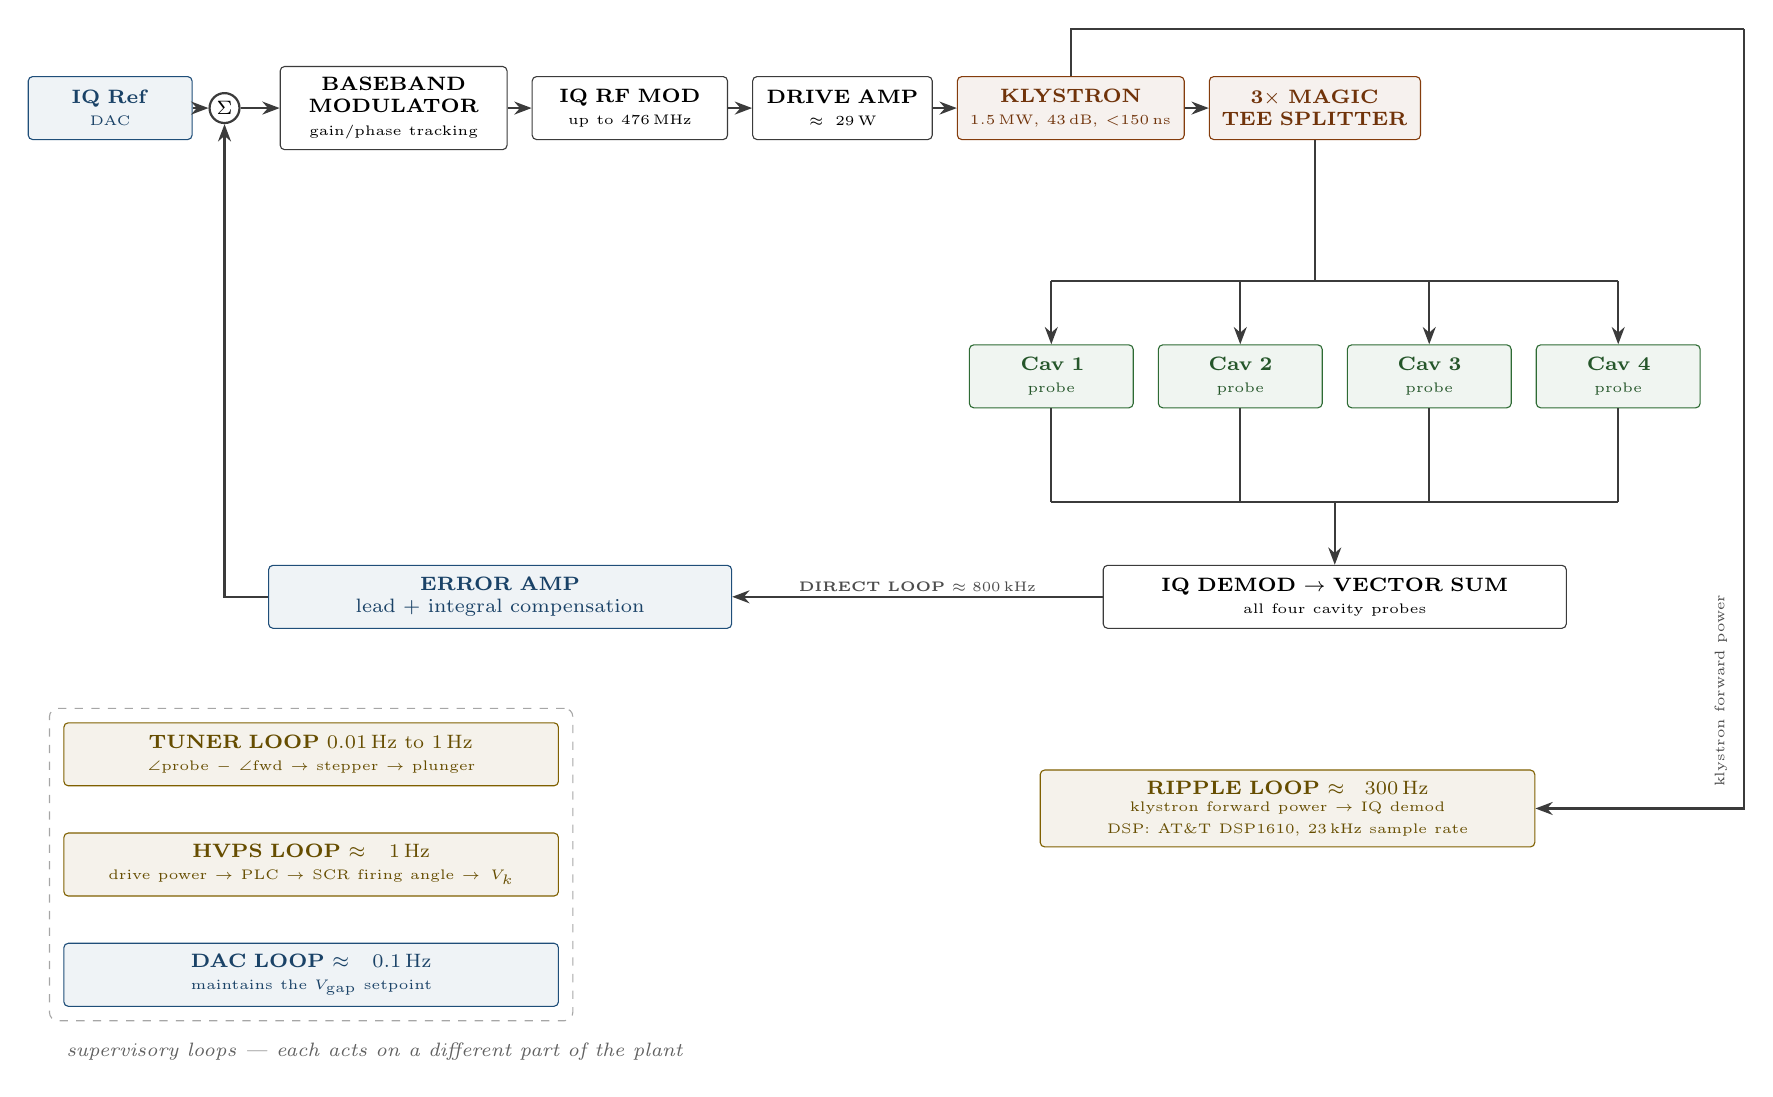
\begin{tikzpicture}[font=\scriptsize, x=1mm, y=1mm]

% ===== forward path ========================================================
\node[ctrl,text width=18mm,anchor=west] (ref) at (0,0)   {\textbf{IQ Ref}\\{\tiny DAC}};
\node[circle,draw=cNeut,thick,fill=white,inner sep=1.2pt] (sum) at (25,0) {$\Sigma$};
\node[blk,text width=26mm,anchor=west] (bb)  at (32,0)   {\textbf{BASEBAND}\\\textbf{MODULATOR}\\{\tiny gain/phase tracking}};
\node[blk,text width=22mm,anchor=west] (mod) at (64,0)   {\textbf{IQ RF MOD}\\{\tiny up to \qty{476}{\mega\hertz}}};
\node[blk,text width=20mm,anchor=west] (drv) at (92,0)   {\textbf{DRIVE AMP}\\{\tiny $\approx\qty{29}{\watt}$}};
\node[pwr,text width=26mm,anchor=west] (kly) at (118,0)  {\textbf{KLYSTRON}\\{\tiny \qty{1.5}{\mega\watt}, \qty{43}{\decibel}, ${<}\qty{150}{\nano\second}$}};
\node[pwr,text width=24mm,anchor=west] (tee) at (150,0)  {\textbf{3$\times$ MAGIC}\\\textbf{TEE SPLITTER}};
\draw[sig] (ref.east) -- (sum.west);
\draw[sig] (sum.east) -- (bb.west);
\foreach \a/\b in {bb/mod, mod/drv, drv/kly, kly/tee}{\draw[sig] (\a.east) -- (\b.west);}

% ===== splitter -> cavities ================================================
\coordinate (fan) at (tee.south |- 0,-22);
\draw[draw=cNeut,thick] (tee.south) -- (fan);
\foreach \i/\n in {0/1, 1/2, 2/3, 3/4}{%
  \pgfmathsetmacro\x{130+\i*24}
  \node[rf,text width=18mm,anchor=north] (c\n) at (\x,-30) {\textbf{Cav \n}\\{\tiny probe}};
  \draw[draw=cNeut,thick] (fan) -- (\x,-22);
  \draw[sig] (\x,-22) -- (c\n.north);
}

% ===== cavity probes -> vector sum =========================================
\foreach \n in {1,2,3,4}{\draw[draw=cNeut,thick] (c\n.south) -- (c\n.south |- 0,-50);}
\draw[draw=cNeut,thick] (c1.south |- 0,-50) -- (c4.south |- 0,-50);

\node[blk,text width=56mm,anchor=north] (dem) at (166,-58)
  {\textbf{IQ DEMOD $\rightarrow$ VECTOR SUM}\\{\tiny all four cavity probes}};
\draw[sig] (166,-50) -- (dem.north);

\node[ctrl,text width=56mm,anchor=north] (err) at (60,-58)
  {\textbf{ERROR AMP}\\ lead $+$ integral compensation};
\draw[sig] (dem.west) -- node[above,tag]
  {\textbf{DIRECT LOOP} $\approx\qty{800}{\kilo\hertz}$} (err.east);
\draw[sig] (err.west) -| (sum.south);

% ===== ripple loop, fed down the reserved right-hand lane ==================
\node[plc,text width=60mm,anchor=north] (rip) at (160,-84)
  {\textbf{RIPPLE LOOP} $\approx\qty{300}{\hertz}$\\
   {\tiny klystron forward power $\rightarrow$ IQ demod\\
    DSP: AT\&T DSP1610, \qty{23}{\kilo\hertz} sample rate}};
\coordinate (tapA) at ($(kly.north)+(0,6)$);
\draw[draw=cNeut,thick] (kly.north) -- (tapA) -- (tapA -| 218,0);
\draw[sig] (tapA -| 218,0) -- (rip.east -| 218,0) -- (rip.east);
\node[tag,rotate=90,anchor=south] at (216.4,-74) {klystron forward power};

% ===== supervisory loops ===================================================
% Grouped rather than wired in: each acts on a different part of the plant, and
% four more return paths would bury the direct loop.
\node[plc,text width=60mm,anchor=north] (tun) at (36,-78)
  {\textbf{TUNER LOOP} \qtyrange{0.01}{1}{\hertz}\\
   {\tiny $\angle$probe $-$ $\angle$fwd $\rightarrow$ stepper $\rightarrow$ plunger}};
\node[plc,text width=60mm,anchor=north] (hv) at (36,-92)
  {\textbf{HVPS LOOP} $\approx\qty{1}{\hertz}$\\
   {\tiny drive power $\rightarrow$ PLC $\rightarrow$ SCR firing angle $\rightarrow V_k$}};
\node[ctrl,text width=60mm,anchor=north] (dac) at (36,-106)
  {\textbf{DAC LOOP} $\approx\qty{0.1}{\hertz}$\\
   {\tiny maintains the $V_\text{gap}$ setpoint}};
\node[grp,fit=(tun)(hv)(dac),inner sep=5pt] (supbox) {};
\node[lbl,anchor=north west] at ($(supbox.south west)+(1,-1.5)$)
  {supervisory loops --- each acts on a different part of the plant};
\end{tikzpicture}
\end{fitpicture}
\caption{The SPEAR3 RF plant as a control system: the klystron and cavity chain is the plant, the LLRF processor is the controller, and the beam is the principal disturbance.}\label{fig:plant-overview}
\end{figure}

\textbf{Key architectural features:}

\begin{itemize}
\tightlist
\item
  \textbf{Single klystron, four cavities}: One I/Q modulator drives all four cavities simultaneously. Field regulation uses the vector sum of all four cavity probes.
\item
  \textbf{Bandwidth hierarchy}: Direct (800 kHz) ≫ Ripple (300 Hz) ≫ HVPS/Tuner (\textasciitilde1 Hz) ≫ DAC (0.1 Hz) --- natural frequency-domain decoupling.
\item
  \textbf{Analog fast path}: The direct loop operates entirely in analog baseband for minimum delay (\(\sim 270\)--500 ns total loop delay).
\end{itemize}

\subsection{RF Cavity as a Narrowband Resonator}\label{sec:cavity}


\subsubsection{Equivalent Circuit}\label{sec:cavity-circuit}


Near its fundamental mode at \(\omega_0 = 2\pi \times 476.3\;\text{MHz}\), each cavity is modeled as a parallel RLC circuit. The cavity parameters (per cavity, linac convention \(R_s = V^2/2P\)):

\begin{longtable}[]{@{}Q{\dimexpr 0.3774\linewidth-1.50\tabcolsep\relax}Q{\dimexpr 0.4151\linewidth-1.50\tabcolsep\relax}Q{\dimexpr 0.1321\linewidth-1.50\tabcolsep\relax}Q{\dimexpr 0.0755\linewidth-1.50\tabcolsep\relax}@{}}
\toprule\noalign{}
Parameter & Symbol & Value & Unit \\
\midrule\noalign{}
\endhead
\bottomrule\noalign{}
\endlastfoot
Resonant frequency & \(f_0\) & ≈ 476.3 & MHz \\
Shunt impedance & \(R_s\) & 3.73 & MΩ \\
Unloaded Q & \(Q_0\) & 32,000 & --- \\
Loaded Q & \(Q_L\) & 6,700 & --- \\
Coupling coefficient & \(\beta = Q_0/Q_\text{ext}\) & 3.78 & --- \\
\end{longtable}

\begin{keynote}
\textbf{Traceability note}: \(R_s = 3.73\) MΩ and \(Q_0 = 32{,}000\) are taken directly from \R{6}, which reports \(\beta_\text{actual} = 3.72\) and \(\beta_\text{optimum} = 3.84\) for PEP-II HER, giving \(Q_L = 6{,}780\). The value \(\beta = 3.78\) used here is a derived operating point (intermediate between actual and optimum) consistent with \(Q_L \approx 6{,}700\) via \(Q_L = Q_0/(1+\beta) = 32{,}000/4.78 = 6{,}695\); Doc~L quotes the \R{6} value \(Q_L = 6{,}780\) directly, and the 1\% difference is immaterial to every result below. \R{1} reports \(R_s = 3.8\) MΩ in the accelerator convention (\(= 2 \times R_s^\text{linac} = 7.6\) MΩ, consistent with \(R_a = 7.5\) MΩ in \R{6}). Cavity geometry and measured impedance spectra are in \R{7} and \R{17}.
\end{keynote}

\subsubsection{Cavity Transfer Function}\label{sec:cavity-tf}


The cavity voltage response to a driving current near resonance:

\begin{equation}\label{eq:cav-tf}
H_\text{cav}(s) = \frac{R_s \,\omega_{1/2}}{s + \omega_{1/2} + j\Delta\omega}
\end{equation}

where \(\omega_{1/2} = \omega_0/(2Q_L)\) is the cavity half-bandwidth. The \textbf{impedance seen by the beam} at frequency offset \(\Delta\omega\) from \(\omega_\text{RF}\):

\begin{equation}\label{eq:cav-imp}
Z_\text{cav}(\Delta\omega) = \frac{R_s}{1 + j\,2Q_L\,\Delta\omega/\omega_0}
\end{equation}

\textbf{Cavity half-bandwidth:}

\begin{equation}\label{eq:cav-bw}
\Delta f_{1/2} = \frac{f_0}{2Q_L} = \frac{476.3\;\text{MHz}}{2 \times 6700} = 35.5\;\text{kHz}
\end{equation}

This determines the cavity natural response time \(\tau_\text{cav} = 1/(2\pi\Delta f_{1/2}) \approx 4.5\;\mu\text{s}\).

\subsubsection{Beam Loading --- Steady-State Phasor Analysis}\label{sec:beam-loading}


A bunched beam of DC current \(I_b\) presents a fundamental RF current \(I_{b1} = 2I_b\) to the cavity, so at 500 mA the cavity sees \qty{1.0}{\ampere} at the RF frequency. Its steady-state induced voltage in the \emph{loaded} cavity, on resonance, is

\begin{equation}\label{eq:vb-res}
V_{b,\text{res}} = \frac{I_{b1} R_s}{1+\beta} = \frac{1.0\;\text{A} \times 3.73\;\text{M}\Omega}{4.78} = 0.78\;\text{MV}
\end{equation}

--- comparable to the \qty{712}{\kilo\volt} the generator is asked to establish. The sharper statement of the same fact is the power split: the beam draws 1.88 times as much power as the cavity walls dissipate (\crefrange{eq:pwall}{eq:pbeam}). \textbf{Beam loading, not wall loss, is what sets the design of this station.}

\textbf{Synchronous phase} --- In the convention where \(\phi_s\) is measured from the voltage crest (SLAC convention, used throughout this document):

\begin{equation}\label{eq:phis}
V_\text{RF} \cos\phi_s = U_0
\end{equation}

\begin{equation}\label{eq:phis-eval}
\cos\phi_s = \frac{U_0}{V_\text{RF}} = \frac{1.02\;\text{MeV}}{2.85\;\text{MV}} = 0.358 \implies \phi_s \approx 69.0^\circ
\end{equation}

Note: \(\sin\phi_s = \sin(69.0^\circ) = 0.934\), which appears in the beam loading compensation formulas below.

\textbf{Synchrotron frequency}:

\begin{equation}\label{eq:nus}
\nu_s = \sqrt{\frac{h\,\alpha_c\,V_\text{RF}\,\sin\phi_s}{2\pi\,E_0}}
\end{equation}

\begin{keynote}
With \(V_\text{RF} = 2.85\) MV, \(\sin\phi_s = 0.934\) and \(E_0\) expressed in the same units as \(V_\text{RF}\) (\(E_0 = 3000\) MeV): \(\nu_s = \sqrt{372 \times 0.00118 \times 2.85 \times 0.934 \,/\, (2\pi \times 3000)} \approx 0.0079\), giving \(f_s = \nu_s \, f_\text{rev} \approx 10.1\) kHz. Published values: \(Q_s = 0.008\) \R{1}, \(\nu_s = 0.007\) \R{3} --- the range reflects differences in operational \(V_\text{RF}\) and \(\alpha_c\) across lattice configurations. For control design, the key constraint is that the direct loop bandwidth (\(\sim 800\) kHz) \(\gg f_s\).
\end{keynote}

\textbf{Optimum detuning} --- The cavity is detuned so that its susceptance cancels the reactive part of the beam-induced current, leaving the generator driving a real load. Writing \(G = 1/R_s\) for the cavity conductance (so that \(P_\text{wall} = \tfrac{1}{2}V_\text{gap}^2 G\), consistent with \cref{eq:pwall}), the reactive balance \(V_\text{gap}\,G\tan\psi_0 + I_{b1}\sin\phi_s = 0\) gives

\begin{equation}\label{eq:psi-opt}
\tan\psi_{0,\text{opt}} = -\frac{I_{b1}\,R_s\,\sin\phi_s}{V_\text{gap}}
  = -\frac{1.0 \times 3.73 \times 10^{6} \times 0.934}{712 \times 10^{3}} = -4.89
\end{equation}

Here \(\psi_0\) is referred to the \emph{unloaded} bandwidth. The angle the tuner loop actually measures --- the phase between the cavity probe and the forward wave --- is referred to the \emph{loaded} bandwidth, and the two are related by \(\tan\psi_L = \tan\psi_0/(1+\beta)\):

\begin{equation}\label{eq:psi-opt-eval}
\tan\psi_{L,\text{opt}} = \frac{-4.89}{1 + 3.78} = -1.02
\quad\Longrightarrow\quad
\psi_{L,\text{opt}} \approx -45.7^\circ
\end{equation}

\begin{keynote}
\textbf{Derivation note}: \Cref{eq:psi-opt} is the condition that the reactive component of the generator current vanish, which minimizes the power reflected at the input coupler. Two factors must be carried correctly and are easy to lose. \textbf{(i)} A bunched beam of DC current \(I_b\) presents a \emph{fundamental} RF current \(I_{b1} = 2I_b\) to the cavity; it is \(I_{b1}\), not \(I_b\), that appears in the reactive balance. \textbf{(ii)} The cavity conductance in the circuit convention \(P_\text{wall} = V_\text{gap}^2/(2R_s)\) is \(G = 1/R_s\). An equivalent and convenient form uses the geometry factor \(R/Q = R_s/Q_0 = \qty{116.6}{\ohm}\), which removes \(Q\) from the expression entirely and is the form used in \cref{eq:df-opt}. The result is cross-checked by the power split: \(I_{b1}R_s\cos\phi_s/V_\text{gap} = 1.88 = P_\text{beam}/P_\text{wall}\), matching \crefrange{eq:pwall}{eq:pbeam} exactly \R{10}, \R{11}, \R{12}, \R{13}.
\end{keynote}

\textbf{Optimum frequency detuning} --- converting the unloaded angle to a frequency offset with \(\tan\psi_0 = 2Q_0\Delta f/f_0\):

\begin{equation}\label{eq:df-opt}
\Delta f_\text{opt} = \frac{f_0}{2Q_0}\tan\psi_{0,\text{opt}}
  = -\frac{(R/Q)\,I_{b1}\,\sin\phi_s\,f_0}{2\,V_\text{gap}}
  = -\frac{116.6\;\Omega \times 1.0\;\text{A} \times 0.934 \times 476.3\;\text{MHz}}{2 \times 712\;\text{kV}}
  \approx -36.4\;\text{kHz}
\end{equation}

The cavity must therefore be tuned about \qty{36}{\kilo\hertz} \textbf{below} \(f_\text{RF}\) at 500 mA --- roughly one cavity half-bandwidth \eqref{eq:cav-bw}, which is why the detuning angle comes out near \(-45^\circ\). \Cref{fig:beam-loading-phasor} shows the resulting steady-state phasor balance; \cref{sec:transient} follows what happens when the beam current or \(f_\text{RF}\) moves away from this operating point.

\begin{figure}[tbp]
\centering
\begin{fitpicture}% !TeX root = ../P_rf_physics_and_plant.tex
% Beam loading phasor diagram, drawn at the real angles: the synchronous phase
% is 69 deg from the voltage crest and the optimum detuning angle is -68 deg.
% Vector lengths are to scale at 0.035 mm/kV, so V_b,res really is 2.6x V_gap.
% Every label sits at its vector's TIP so that nothing overlaps the arrows.
\begin{tikzpicture}[font=\scriptsize, x=1mm, y=1mm,
                    ph/.style={-{Stealth[length=2.6mm]},line width=1.1pt}]
\def\s{0.035}

\draw[draw=black!45] (-74,0) -- (44,0) node[right,lbl]{Real};
\draw[draw=black!45] (0,-46) -- (0,30) node[above,lbl]{Imaginary};

% cavity gap voltage, on the real axis
\draw[ph,draw=cRf] (0,0) -- (712*\s,0);
\node[tag,text=cRf,anchor=west,align=left] at (712*\s+2,2.5)
  {$V_\text{gap}=\qty{712}{\kilo\volt}$};

% beam-induced voltage at resonance: 2.6x larger, and opposing
\draw[ph,draw=cPwr] (0,0) -- (-1865*\s,0);
\node[tag,text=cPwr,anchor=west,align=left] at (-1865*\s,4)
  {$V_{b,\text{res}}=I_b R_s=\qty{1865}{\kilo\volt}$};

% synchronous phase, measured from the crest
\draw[draw=cCtrl,densely dashed] (0,0) -- (69:30);
\draw[draw=cCtrl] (14,0) arc (0:69:14);
\node[tag,text=cCtrl,anchor=south west] at (69:31) {$\phi_s=69^\circ$};

% generator voltage at the optimum detuning angle
\draw[ph,draw=cPlc] (0,0) -- (-68:40);
\node[tag,text=cPlc,anchor=north west,align=left] at (-68:41)
  {$V_\text{gen}$ --- generator voltage};
\draw[draw=cPlc] (22,0) arc (0:-68:22);
\node[tag,text=cPlc,anchor=west] at (24,-12)
  {$\psi_\text{opt}=-68^\circ$ (detuning angle)};
\end{tikzpicture}
\end{fitpicture}
\caption{Beam loading phasor diagram in steady state at \qty{500}{\milli\ampere}. The cavity is detuned so that the generator sees a real load: the reactive part of the beam-induced voltage is cancelled by the detuning angle $\psi$.}\label{fig:beam-loading-phasor}
\end{figure}

\textbf{Required generator power per cavity} --- At optimum coupling (\(\beta_\text{opt}\)) and optimum detuning (\(\psi_\text{opt}\)), the minimum generator power per cavity is the sum of cavity wall losses and beam power:

\begin{equation}\label{eq:pgen}
P_\text{gen/cav} = P_\text{wall} + \frac{P_\text{beam}}{n_\text{cav}} = \frac{V_\text{gap}^2}{2R_s} + \frac{I_b \, U_0}{n_\text{cav}}
\end{equation}

\textbf{Evaluation:}

\begin{equation}\label{eq:pwall}
P_\text{wall} = \frac{V_\text{gap}^2}{2R_s} = \frac{(712\;\text{kV})^2}{2 \times 3.73\;\text{M}\Omega} = 68\;\text{kW/cavity}
\end{equation}

\begin{equation}\label{eq:pbeam}
\frac{P_\text{beam}}{n_\text{cav}} = \frac{I_b \, U_0}{n_\text{cav}} = \frac{0.5\;\text{A} \times 1.02\;\text{MeV}}{4} = 127.5\;\text{kW/cavity}
\end{equation}

\begin{equation}\label{eq:pgen-eval}
P_\text{gen/cav} = 68 + 127.5 \approx 196\;\text{kW/cavity}
\end{equation}

\textbf{Total RF power}: \(4 \times 195.6 \approx 782\) kW --- within the 1.5 MW klystron capacity, leaving \(\sim 48\%\) headroom. The measured forward power at 500 mA is \(\sim 200\) kW/cavity, consistent with this calculation (the small excess accounts for reflected power at non-ideal coupling).

\begin{keynote}
\textbf{Note}: \cref{eq:pgen} is the minimum-power condition at optimum coupling. In the general case with arbitrary coupling \(\beta\) and detuning \(\psi\), the generator power includes reflected power terms. The important identity is that beam power per cavity \(= I_b V_\text{gap}\cos\phi_s = I_b \, U_0/n_\text{cav}\).
\end{keynote}

\subsection{Klystron as the Actuator}\label{sec:klystron}


For control analysis, the klystron is modeled as:

\begin{equation}\label{eq:kly-tf}
G_\text{kly}(s) = K_\text{kly} \cdot e^{-s\tau_\text{kly}}
\end{equation}

where \(K_\text{kly}\) is the small-signal gain and \(\tau_\text{kly} < 150\) ns.

\begin{longtable}[]{@{}Q{\dimexpr 0.3704\linewidth-1.33\tabcolsep\relax}Q{\dimexpr 0.3889\linewidth-1.33\tabcolsep\relax}Q{\dimexpr 0.2407\linewidth-1.33\tabcolsep\relax}@{}}
\toprule\noalign{}
Parameter & Value & Unit \\
\midrule\noalign{}
\endhead
\bottomrule\noalign{}
\endlastfoot
Maximum output power & 1.5 MW & CW \\
Gain & 43 dB (min) & --- \\
Bandwidth & 5 MHz & −3 dB \\
Group delay & \(< 150\) ns & --- \\
Perveance \(K = I_k/\lvert V_k \rvert^{3/2}\) & \(\sim 1.0 \times 10^{-6}\) & \(\text{A/V}^{3/2}\) \\
\end{longtable}

Klystron ratings are from \R{1}; the perveance follows from the HVPS operating point of \cref{sec:hvps-params} (\(-77\) kV at 22 A gives \(K = 22/(7.7\times10^4)^{3/2} = 1.03 \times 10^{-6}\;\text{A/V}^{3/2}\)) and agrees with the measured cathode readbacks recorded in Doc~L. The value \(2.0 \times 10^{-6}\) that appears in the HVPS simulation configuration \R{23} is not consistent with that operating point and is not used here.

\textbf{Saturation model:}

\begin{equation}\label{eq:kly-sat}
P_\text{out} = P_\text{sat} \cdot \frac{P_\text{in}/P_\text{in,sat}}{1 + P_\text{in}/P_\text{in,sat}}
\end{equation}

\textbf{AM-PM conversion} --- klystron output phase sensitivity to cathode voltage \R{15}:

\begin{equation}\label{eq:kly-ampm}
\Delta\phi_\text{kly} \propto \frac{\Delta V_k}{V_k}
\end{equation}

\subsection{Loop Delay Budget --- The Fundamental Bandwidth Ceiling}\label{sec:delay-budget}


The delay around the direct loop sets a hard ceiling on its crossover frequency. A pure delay \(\tau_d\) contributes a phase lag \(-2\pi f \tau_d\) that grows without bound, so the usable crossover is fixed by the delay alone:

\begin{equation}\label{eq:fc-max}
\boxed{f_{c,\text{max}} \approx \frac{1}{4\tau_d}}
\end{equation}

This is the single most important constraint in the entire control design. It is an engineering rule of thumb: at \(f_c = 1/(4\tau_d)\) the transport delay alone has consumed \(90^\circ\) of phase, which leaves a workable margin once the lead compensator has offset the cavity pole. It is not a stability proof --- the actual margin must be read from the gain/phase budget in \cref{sec:loop-direct}.

\begin{longtable}[]{@{}Q{\dimexpr 0.4340\linewidth-1.33\tabcolsep\relax}Q{\dimexpr 0.2830\linewidth-1.33\tabcolsep\relax}Q{\dimexpr 0.2830\linewidth-1.33\tabcolsep\relax}@{}}
\toprule\noalign{}
Component & Legacy (analog) & LLRF9 (digital) \\
\midrule\noalign{}
\endhead
\bottomrule\noalign{}
\endlastfoot
Klystron group delay & \(< 150\) ns & \(< 150\) ns \\
I/Q modulator & \(< 5\) ns & \(< 5\) ns \\
Cable propagation & \(\sim 50\) ns & \(\sim 50\) ns \\
Electronics/computation & \(\sim 300\) ns & \(\sim 65\) ns \\
\textbf{Total} \(\tau_d\) & \textbf{\(\sim 500\) ns} & \textbf{\(\sim 270\) ns} \\
\(f_{c,\text{max}}\) & \textbf{\(\sim 500\) kHz} & \textbf{\(\sim 926\) kHz} \\
\end{longtable}

\textbf{Note}: The 270 ns figure for the LLRF9 column is the direct-loop delay quoted in the vendor manual \R{4}; it is assumed here to be the total loop delay as itemised above [to be confirmed].

\subsection{Complete Open-Loop Plant Transfer Function}\label{sec:plant-ol}


\begin{equation}\label{eq:plant}
G_\text{plant}(s) = G_0 \cdot H_\text{cav}(s) \cdot e^{-s\tau_d} = \frac{G_0 \,\omega_{1/2}}{s + \omega_{1/2} + j\Delta\omega}\; e^{-s\tau_d}
\end{equation}

The cavity bandwidth (\(35.5\) kHz) and the loop delay together define the limits of what feedback can achieve.

\begin{center}\rule{0.5\linewidth}{0.5pt}\end{center}

\section{I/Q Signal Processing Framework}\label{sec:iq}


\subsection{Baseband I/Q Representation}\label{sec:iq-baseband}


All RF feedback loops use baseband In-phase and Quadrature (I/Q) techniques:

\begin{equation}\label{eq:iq-def}
V_\text{RF}(t) =A(t)\cos[\omega_\text{RF}t + \phi(t)] = I(t)\cos(\omega_\text{RF}t) - Q(t)\sin(\omega_\text{RF}t)
\end{equation}

where \(I(t) = A(t)\cos\phi(t)\) and \(Q(t) = A(t)\sin\phi(t)\), with inverse relations:

\begin{equation}\label{eq:iq-aphi}
A(t) = \sqrt{I^2 + Q^2}\,,\qquad \phi(t) = \text{atan2}(Q, I)
\end{equation}

\subsection{Baseband I/Q Modulator}\label{sec:iq-modulator}


The I/Q modulator performs a scaled rotation:

\begin{equation}\label{eq:iq-mod}
\begin{pmatrix} I_\text{out} \\ Q_\text{out} \end{pmatrix} = G \begin{pmatrix} \cos\theta & -\sin\theta \\ \sin\theta & \cos\theta \end{pmatrix} \begin{pmatrix} I_\text{in} \\ Q_\text{in} \end{pmatrix}
\end{equation}

\textbf{Implementation}: Each baseband I/Q modulator uses four AD834 four-quadrant multipliers (DC to 500 MHz) \R{18} plus two EL2073 summing amplifiers to implement the 2×2 matrix. Group delay \(< 5\) ns, full-power bandwidth \(> 40\) MHz, dynamic range \(> 50\) dB \R{14}, \R{15}.

\textbf{SPEAR3 modulator count}: 4 cavity combining modulators (one per probe) + 1 drive modulator (direct loop gain/phase) = \textbf{5 baseband I/Q modulators}, with associated Octal DAC channels on the RFP module for the 2×2 matrix coefficients.

\begin{keynote}
\textbf{PEP-II comparison}: The PEP-II HER system used 7 baseband I/Q modulators (4 cavity combining + 1 direct loop + 1 comb filter adjust + 1 ripple) with 56 DAC channels \R{15}. SPEAR3 requires fewer because: (a) the comb loop is not used, (b) the ripple correction is applied via DSP rather than a dedicated modulator. The AD834 multipliers and EL2073 op-amps are the same components.
\end{keynote}

\subsection{I/Q Demodulation}\label{sec:iq-demod}


RF signals are converted to baseband I/Q using \(+13\) dBm demodulators. Outputs: AC-coupled into \(50\;\Omega\), low-pass filtered (\(F_c = 225\) MHz), video amplified (17 dB) to \(\pm 1\) V.

\subsection{Cavity Probe Vector Sum}\label{sec:iq-vectorsum}


Each of the 4 cavity probe signals is demodulated to I/Q and combined through a programmable combining network (4 I/Q baseband modulators + 2 summing amplifiers on the RFP module) to form the \textbf{total accelerating RF vector}. The DAC weights for each modulator set the complex gain for each cavity\textquotesingle s contribution to the vector sum.

\subsection{Error Signal Generation}\label{sec:iq-error}


\begin{equation}\label{eq:err}
\vec{E} = \vec{V}_\text{ref} - \vec{V}_\text{probe}
\end{equation}

\begin{equation}\label{eq:drive}
\vec{V}_\text{drive} = G_\text{loop} \cdot \vec{E} = G_\text{loop}\left(\vec{V}_\text{ref} - \vec{V}_\text{probe}\right)
\end{equation}

The error signals \(\Delta I\), \(\Delta Q\) are then combined with the reference \(I, Q\) to compute the rotation angle and multipliers of \cref{eq:iq-mod} for cavity field regulation. The I/Q baseband representation developed in this section is used throughout \crefrange{sec:disturbances}{sec:performance} to express all loop transfer functions in the complex baseband domain \R{14}, \R{15}.

\begin{center}\rule{0.5\linewidth}{0.5pt}\end{center}

\section{Disturbance Analysis and Control Problem Statement}\label{sec:disturbances}


\textbf{The control architecture follows inevitably from the disturbance landscape.}

\subsection{Disturbance Taxonomy}\label{sec:dist-taxonomy}
\raisebox{0pt}[0pt][0pt]{\hypertarget{dist:table}{}}

The nine disturbance classes below are referred to as D1--D9 throughout the rest of this document; each one is the reason that a particular loop exists.

\begin{longtable}[]{@{}Q{\dimexpr 0.0200\linewidth-1.60\tabcolsep\relax}Q{\dimexpr 0.2658\linewidth-1.60\tabcolsep\relax}Q{\dimexpr 0.2242\linewidth-1.60\tabcolsep\relax}Q{\dimexpr 0.2242\linewidth-1.60\tabcolsep\relax}Q{\dimexpr 0.2658\linewidth-1.60\tabcolsep\relax}@{}}
\toprule\noalign{}
\# & Disturbance & Frequency & Magnitude & Impact \\
\midrule\noalign{}
\endhead
\bottomrule\noalign{}
\endlastfoot
D1 & Beam loading (steady-state) & DC & \(V_b = 0.78\) MV/cavity & Dominates voltage budget \\
D2 & Beam loading (transient) & DC--100 kHz & Growth rates \(< T_\text{rev}\) & Longitudinal instability \\
D3 & Robinson instability & \(f_s \sim 10\) kHz \eqref{eq:nus} & Exponential growth & Beam loss \\
D4 & Coupled-bunch modes & \(n \cdot f_\text{rev}\) & \(1/\tau_{cb}\) & Beam oscillation \\
D5 & HVPS ripple & 360, 720, 1080\ldots{} Hz & \(< 1\%\) P-P voltage & Phase modulation \\
D6 & Klystron gain drift & 0.01--1 Hz & up to 7 dB & Loop gain variation \\
D7 & Microphonics & 1--300 Hz & \(\Delta f \sim 1\)--\(10\) Hz & Cavity detuning \\
D8 & Thermal detuning (cavity) & \(< 0.01\) Hz & \(\Delta f \sim 1\)--\(100\) Hz & Slow frequency drift \\
D9 & Ring circumference thermal drift & Seasonal (\(\ll 0.001\) Hz) & \(\Delta f_{RF} \sim 4\) kHz/year & Secular tuner setpoint migration \\
\end{longtable}

\subsection{D1/D2: Beam Loading --- The Dominant Disturbance}\label{sec:d1d2}


\textbf{D1 --- Steady-state beam loading}: Each bunch extracts energy from the cavity field. The beam-induced voltage \(V_{b,\text{res}} = 0.78\) MV per cavity \eqref{eq:vb-res} is comparable to the gap voltage itself, and the beam draws 1.88 times the wall-loss power. Without active compensation the generator would also have to supply the beam's reactive loading. Detuning the cavity (\cref{sec:beam-loading}) brings that reactive component to zero at the operating current, but any current deviation re-creates the mismatch --- see \cref{sec:transient}.

\textbf{D2 --- Transient beam loading}: Current transients (injection, ion-clearing gap, bunch-by-bunch variations) cause rapid changes in the beam-induced voltage. These transients drive cavity field oscillations at frequencies up to \(\sim f_\text{rev}\).

\textbf{How feedback suppresses D1/D2}: The direct feedback loop divides the cavity impedance seen by the beam by the return difference $1 + G_\text{OL}$ (\cref{eq:zeff}).

At DC and low frequencies where \(|G_\text{OL}| \gg 1\) (proportional gain \(\sim 15\) dB + integrator), the impedance reduction is \(\sim 40\) dB (\(\times 100\)). This has two physical effects:

\begin{enumerate}
\def\labelenumi{\arabic{enumi}.}
\item
  \textbf{Voltage regulation}: The beam-induced voltage perturbation \(\Delta V_b = \Delta I_b \cdot Z_\text{eff}\) is reduced by the loop gain. A 1\% current transient that would cause \(\sim 19\) kV field perturbation without feedback produces only \(\sim 190\) V with 40 dB impedance reduction.
\item
  \textbf{Stability}: The beam-cavity interaction becomes stable because the reduced impedance eliminates the conditions for exponential growth. The \textbf{growth rate} for coupled-bunch instability from the fundamental mode \R{15}:
\end{enumerate}

\begin{equation}\label{eq:cb-growth}
\frac{1}{\tau} = \frac{I_b\,\alpha_c\,f_\text{RF}}{2\,\nu_s\,\beta^2\,(E/e)}\;R_{cb}
\end{equation}

where \(R_{cb} = \sum_n \text{Re}\left[Z_\text{eff}(\omega_\text{RF} + n\omega_\text{rev} + \omega_s) - Z_\text{eff}(\omega_\text{RF} + n\omega_\text{rev} - \omega_s)\right]\).

With feedback, \(Z_\text{eff}\) replaces \(Z_\text{cav}\) in the sum, reducing growth rates by the same factor as the impedance reduction. \textbf{Without feedback}, the peak cavity impedance of \(\sim 750\;\text{k}\Omega\) produces growth rates faster than \(T_\text{rev} \approx 0.78\;\mu\text{s}\). This single fact drove the PEP-II system design to include multiple feedback loops \R{15}. The steady-state phasor balance that the detuning establishes is drawn in \cref{fig:beam-loading-phasor}.

\subsection{D3: Robinson Instability}\label{sec:d3}


\textbf{Robinson stability criterion} (above transition):

\begin{equation}\label{eq:robinson-crit}
\text{Re}\{Z_\text{eff}(\omega_\text{RF} + \omega_s)\} < \text{Re}\{Z_\text{eff}(\omega_\text{RF} - \omega_s)\}
\end{equation}

\textbf{Robinson growth rate:}

\begin{equation}\label{eq:robinson-rate}
\frac{1}{\tau_\text{Rob}} = \frac{\alpha_c\,\omega_\text{rev}\,I_b}{4\,\omega_s\,(E/e)} \left[\text{Re}\{Z(\omega_\text{RF} + \omega_s)\} - \text{Re}\{Z(\omega_\text{RF} - \omega_s)\}\right]
\end{equation}

Direct feedback reduces \(Z_\text{eff} = Z_\text{cav}/(1 + G_\text{OL})\), reducing the growth rate by the same factor \R{11}, \R{13}, \R{16}.

\subsection{D4: Coupled-Bunch Modes}\label{sec:d4}


With \(h = 372\) RF buckets the beam supports 372 coupled-bunch modes; each mode \(m\) is driven by the impedance sampled at revolution harmonics:

\begin{equation}\label{eq:cb-mode}
\frac{1}{\tau_m} = \frac{\alpha_c\,\omega_\text{rev}\,I_b}{4\,\omega_s\,(E/e)}\sum_p\left[\text{Re}\{Z((ph+m)\omega_\text{rev}+\omega_s)\} - \text{Re}\{Z((ph+m)\omega_\text{rev}-\omega_s)\}\right]
\end{equation}

\textbf{Physics of the comb filter}: The comb filter provides additional impedance reduction at revolution frequency harmonics --- precisely where beam-driven modes exist --- without raising gain, and therefore noise, at the frequencies between harmonics. Its transfer function \eqref{eq:comb} has gain peaks at integer multiples of \(f_\text{rev}\), giving the characteristic comb-tooth response of \cref{fig:comb-response}.

\begin{figure}[tbp]
\centering
\begin{fitpicture}% !TeX root = ../P_rf_physics_and_plant.tex
% Comb filter response.  Drawn from the digital comb magnitude
%   M(f) = (1-K) / sqrt(1 - 2K cos(2 pi f/f_rev) + K^2),
% plotted as the resulting loop gain 1 + G*M(f).  K and G are stated in the
% caption: this figure shows the SHAPE, not fitted SPEAR3 parameters.
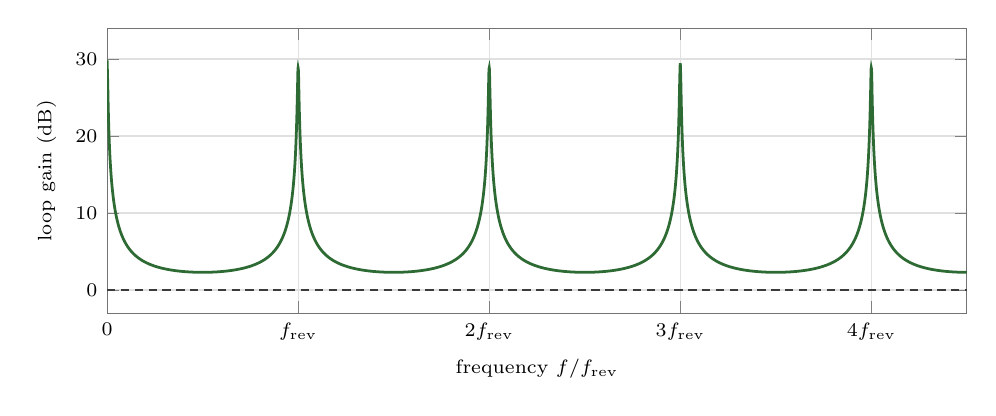
\begin{tikzpicture}
\begin{axis}[
  width=125mm, height=52mm,
  xlabel={frequency $f/f_\text{rev}$},
  ylabel={loop gain (dB)},
  domain=0:4.5, samples=1600,
  xmin=0, xmax=4.5, ymin=-3, ymax=34,
  xtick={0,1,2,3,4},
  xticklabels={$0$,$f_\text{rev}$,$2f_\text{rev}$,$3f_\text{rev}$,$4f_\text{rev}$},
  ytick={0,10,20,30},
  grid=major, grid style={draw=black!12},
  tick label style={font=\scriptsize}, label style={font=\scriptsize},
  axis line style={draw=black!55},
]
\addplot[draw=cRf,line width=1pt,smooth]
  {20*log10(1 + 30*(1-0.98)/sqrt(1 - 2*0.98*cos(360*x) + 0.98^2))};
\addplot[draw=cNeut,densely dashed,line width=0.7pt,samples=2]{0};
\end{axis}
\end{tikzpicture}
\end{fitpicture}
\caption{Comb filter response. The peaks sit at multiples of the revolution frequency, one per coupled-bunch mode; between them the gain returns towards unity, so the filter adds no broadband noise. Drawn from the digital comb magnitude with pole radius $K=0.98$ and comb gain 30 to show the characteristic shape --- these are not fitted SPEAR3 values.}\label{fig:comb-response}
\end{figure}

\textbf{Why SPEAR3 does not need the comb filter}: The key ratio is \(f_\text{rev}/\Delta f_{1/2}\):

\begin{itemize}
\item
  \textbf{SPEAR3}: \(f_\text{rev} = 1.28\) MHz \(\gg \Delta f_{1/2} = 35.5\) kHz → ratio \(\approx 36\). In this regime, only the central RF harmonic lies within the cavity bandwidth, while all revolution sidebands are many cavity linewidths away and therefore do not significantly couple through the cavity impedance. The cavity effectively behaves as a narrowband filter, responding primarily to the carrier component of the beam current.
\item
  As a result, beam-induced disturbances at revolution harmonics are not directly amplified by the cavity, and the interaction is dominated by the fundamental RF component. The SPEAR3 beam current is also much lower than PEP-II\textquotesingle s, so the system is correspondingly less sensitive to revolution-harmonic coupling and comb filtering is not necessary for fine control or disturbance rejection.
\item
  \textbf{PEP-II}: \(f_\text{rev} \approx 136\) kHz, comparable to \(\Delta f_{1/2}\) → ratio \(\approx 4\). Although only the central RF harmonic lies strictly within the cavity bandwidth, the nearby revolution harmonics are only a few cavity linewidths away and therefore couple significantly through the cavity impedance.
\item
  As a result, multiple revolution sidebands contribute to the beam--cavity interaction and must be actively controlled at PEP-II. That regime requires a comb filter, which suppresses selectively at the revolution harmonics and so mitigates beam-induced disturbances without the broadband noise amplification a purely wideband loop would introduce.
\end{itemize}

\subsection{D5: HVPS Ripple}\label{sec:d5}


The 12-pulse SCR rectifier produces two families of harmonics:

\textbf{12-pulse fundamental harmonics} (ideal 12-pulse cancellation):

\begin{equation}\label{eq:ripple-12p}
f_\text{12p} = 12n \times f_\text{line} = 720,\;1440,\;2160,\;\ldots\;\text{Hz}
\end{equation}

\textbf{Residual 6-pulse harmonics} (from imperfect phase balance between the two 6-pulse bridges):

\begin{equation}\label{eq:ripple-6p}
f_\text{6p} = 6n \times f_\text{line} = 360,\;720,\;1080,\;\ldots\;\text{Hz}
\end{equation}

The 360 Hz component (the first 6-pulse harmonic, absent in ideal 12-pulse operation) is the \textbf{dominant residual} and the primary target of the ripple loop. Additional low-order harmonics at 60, 120, 180 and 240 Hz may appear at reduced levels (\(\sim 20\)--\(40\) dB below 360 Hz) depending on SCR firing symmetry \R{21}, \R{22}. The ripple couples into the RF field through klystron AM-PM conversion:

\begin{equation}\label{eq:ampm}
\Delta\phi_\text{RF} \sim \frac{\partial P_\text{kly}/\partial V_k}{P_\text{kly}} \cdot \Delta V_\text{ripple}
\end{equation}

\subsection{D6: Klystron Gain Variation}\label{sec:d6}


\textbf{Source of gain variation}: As beam current changes from 0 to 500 mA, the HVPS loop adjusts cathode voltage \(V_k\) to maintain the klystron \(\sim 10\%\) below saturation. As \(V_k\) changes, the small-signal gain (slope of the \(P_\text{out}\) vs \(P_\text{in}\) curve) varies by up to \(\sim 7\) dB. This shifts the open-loop gain of the direct feedback loop, potentially affecting stability margins.

\textbf{Gain tracking implementation}: The baseband modulator on the RFP module (4 Gilbert-cell multipliers in a 2×2 matrix) has its matrix coefficients controlled by 12-bit Octal DACs. A slow EPICS loop (\(\sim 1\) Hz) reads the klystron forward power and drive power monitors, computes the current gain, and adjusts the modulator matrix so that the product \(G_\text{modulator} \cdot G_\text{klystron}(V_k)\) stays constant (\cref{sec:loop-gain-tracking}).

The MATLAB calibration routine \texttt{ConfDirect} (initiated from the EPICS feedback panel) performs the initial gain tracking setup by measuring klystron gain at the current operating point and writing the appropriate 2×2 matrix coefficients to the quad DAC.

\begin{keynote}
\textbf{Note}: In PEP-II, the ripple loop also applied gain/phase correction via a dedicated I/Q modulator. At SPEAR3, the ripple loop phase correction is handled by the DSP (AT\&T DSP1610), and the slow gain tracking is handled by the baseband modulator coefficients on the RFP module.
\end{keynote}

\subsection{D7/D8: Microphonics and Thermal Detuning}\label{sec:d7d8}


For normal-conducting copper cavities: microphonic excursions \(< 10\) Hz (negligible vs. \(\Delta f_{1/2} = 35.5\) kHz).

\textbf{Thermal detuning estimation}: The resonant frequency of a copper cavity scales inversely with its linear dimensions: \(\Delta f/f = -\alpha_\text{Cu} \cdot \Delta T\), where \(\alpha_\text{Cu} \approx 16.5 \times 10^{-6}\;/\text{°C}\) is the linear thermal expansion coefficient of copper. For a simple cavity at 476.3 MHz, this gives:

\begin{equation}\label{eq:cav-thermal}
\frac{\partial f_0}{\partial T} \approx -f_0 \cdot \alpha_\text{Cu} = -476.3\;\text{MHz} \times 16.5 \times 10^{-6} \approx -7.9\;\text{kHz/°C}
\end{equation}

\begin{keynote}
\textbf{Note}: This first-principles estimate (\(-7.9\) kHz/°C) applies to the uncooled cavity body. In practice the PEP-II-type cavities at SPEAR3 run on a regulated water-cooling circuit that holds the body temperature to within \(\sim \pm 0.1\)°C, so the \emph{observed} drift referred to the cooling-water setpoint is roughly an order of magnitude smaller --- of order \(-1\) kHz/°C (\cref{sec:tuner-physics}).
\end{keynote}

The tuner loop (\cref{sec:loop-tuner}) tracks both microphonics and thermal drift, maintaining the cavity at the optimum detuning angle \(\psi_\text{opt}\) \eqref{eq:psi-opt-eval}.

\subsection{D9: Ring Circumference Thermal Drift --- Long-Term RF Frequency Migration}\label{sec:d9}


\textbf{Physical origin}: The RF harmonic condition requires the RF operating frequency to equal an integer multiple of the revolution frequency:

\begin{equation}\label{eq:harmonic}
f_\text{RF} = h \cdot f_\text{rev} = \frac{h \cdot c}{C}
\end{equation}

The ring circumference \(C = 234.14\) m is set by the physical path of the beam through the tunnel. As the building structure thermally expands and contracts with seasonal temperature changes, \(C\) varies slowly on a monthly-to-annual timescale. By the harmonic condition, the correct RF operating frequency must shift accordingly. A nominally fixed RF master oscillator becomes progressively detuned from the correct harmonic as the circumference drifts.

\textbf{Measured magnitude at SPEAR3}: The RF operating frequency migrates by approximately \(\lvert\Delta f_\text{RF}\rvert \approx 4\) kHz over one year. Differentiating the harmonic condition at fixed \(h\) gives \(\Delta C/C = -\Delta f_\text{RF}/f_\text{RF}\), so the fractional change in circumference is

\begin{equation}\label{eq:dC-over-C}
\left\lvert \frac{\Delta C}{C} \right\rvert = \left\lvert \frac{\Delta f_\text{RF}}{f_\text{RF}} \right\rvert = \frac{4\;\text{kHz}}{476.3\;\text{MHz}} = 8.4 \times 10^{-6}
\end{equation}

\begin{equation}\label{eq:dC}
\lvert \Delta C \rvert = 8.4 \times 10^{-6} \times 234.14\;\text{m} \approx 2.0\;\text{mm}
\end{equation}

The circumference and the required RF frequency move in \emph{opposite} directions: a warmer, longer tunnel needs a lower \(f_\text{RF}\). A 2 mm annual change in the 234 m circumference is consistent with a tunnel temperature variation of \(\sim\) 0.8°C (concrete/steel: \(\alpha_\text{struct} \approx 10\)--\(12 \times 10^{-6}\)/°C), physically plausible for a building with seasonal HVAC cycling.

\textbf{Contrast with D8 (cavity body thermal detuning)}:

\begin{longtable}[]{@{}Q{\dimexpr 0.1067\linewidth-1.33\tabcolsep\relax}Q{\dimexpr 0.2933\linewidth-1.33\tabcolsep\relax}Q{\dimexpr 0.6000\linewidth-1.33\tabcolsep\relax}@{}}
\toprule\noalign{}
& D8: Cavity thermal detuning & D9: Ring circumference drift \\
\midrule\noalign{}
\endhead
\bottomrule\noalign{}
\endlastfoot
\textbf{Physical origin} & Cavity copper temperature → \(f_0\) shifts & Tunnel/building temperature → \(C\) changes → required \(f_\text{RF}\) shifts \\
\textbf{Rate} & \(-7.9\) kHz/°C \eqref{eq:cav-thermal} & \(\sim 4\) kHz/year (measured operational data) \\
\textbf{Timescale} & Short-term (hourly) & Long-term (seasonal/annual) \\
\textbf{Control variable} & Tuner re-tracks \(f_0\) relative to \(f_\text{RF}\) & Tuner re-converges to new equilibrium as \(f_\text{RF}\) migrates; RF master oscillator updated periodically \\
\end{longtable}

\textbf{Impact on the control system}: The operating detuning \(\Delta f = f_0 - f_\text{RF}\) (\cref{sec:c9-conventions}) defines the tuner equilibrium. Both D8 and D9 shift \(\Delta f\), but from opposite sides --- D8 moves \(f_0\) (cavity geometry changes), while D9 moves \(f_\text{RF}\) (ring geometry changes). The tuner loop (\cref{sec:loop-tuner}) is closed around the detuning angle \(\psi = \arctan(2Q_L \Delta f / f_0)\), so it automatically re-converges to \(\psi_\text{opt}\) when \(f_\text{RF}\) changes, provided:

\begin{enumerate}
\def\labelenumi{\arabic{enumi}.}
\tightlist
\item
  The tuner mechanical range and total step count are sufficient to reach the new equilibrium position.
\item
  The RF master oscillator frequency is updated periodically by feedback system to track the ring operating point.
\end{enumerate}

\subsection{Frequency-Domain Summary: The Disturbance Spectrum}\label{sec:dist-spectrum}


\begin{figure}[tbp]
\centering
\begin{fitpicture}% !TeX root = ../P_rf_physics_and_plant.tex
% Disturbance spectrum on a log frequency axis, with the loop responsible for
% each band.  Drawn on a log axis so the decade separation between adjacent
% loop bandwidths is visible rather than merely asserted.
%
% SIZING.  Keep the total drawn width under about 160 mm.  The axis is only
% 110 mm wide precisely so that the right-hand label column fits inside the
% text block: if the picture overflows, fitpicture shrinks the whole thing and
% the labels become unreadable, which is what happened when the axis was 180 mm
% and the labels ran on a single line.  Two-line labels keep the width down;
% the 14 mm row pitch keeps each label visually attached to its own bar.
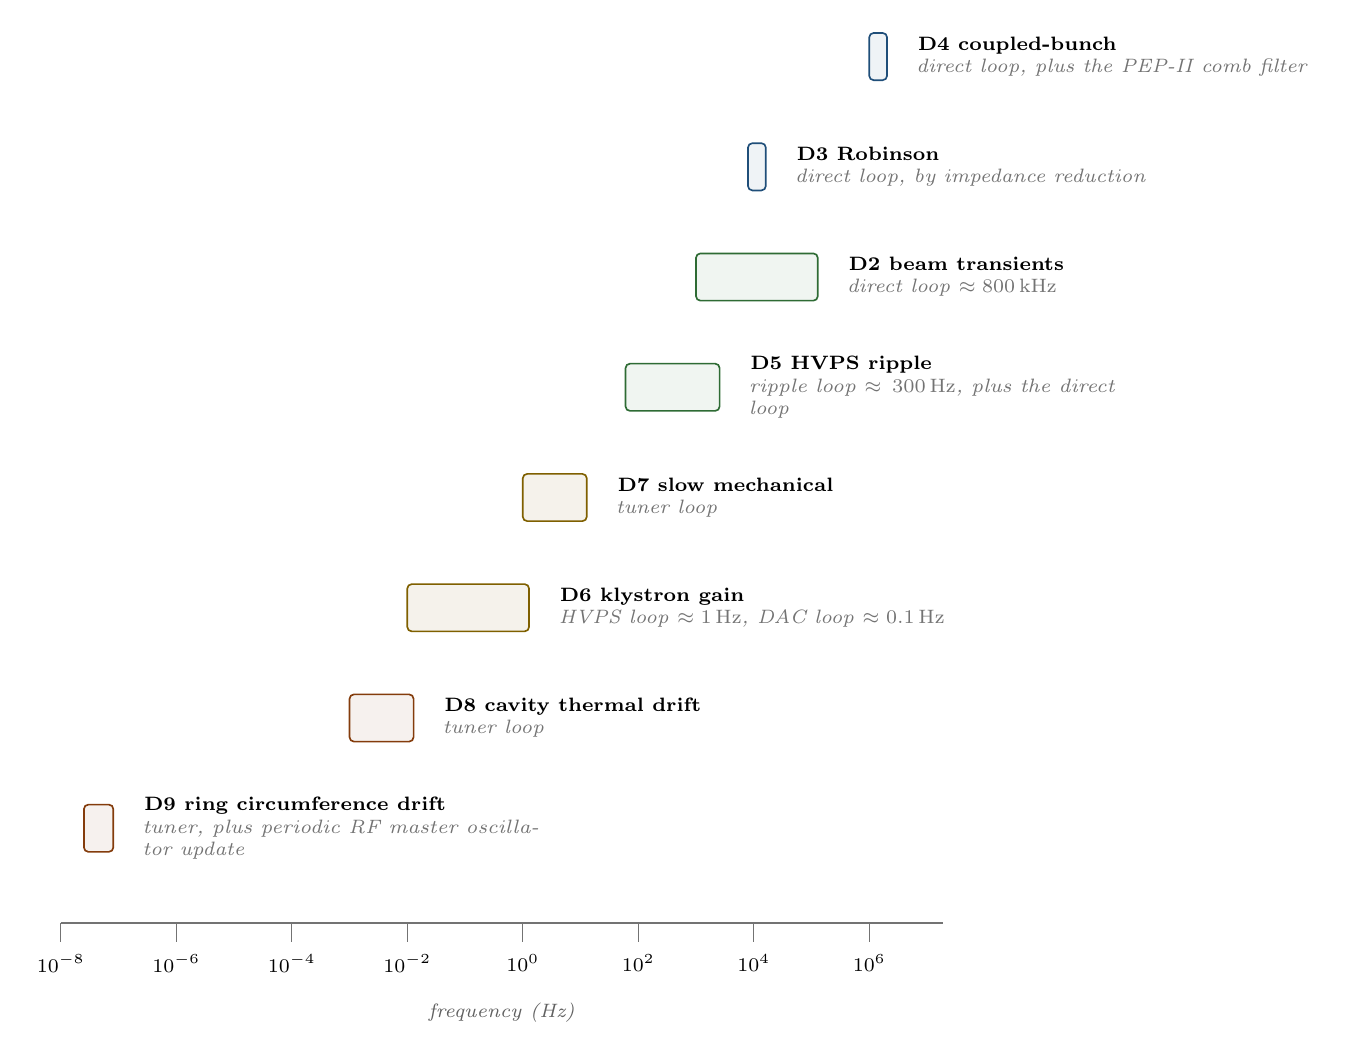
\begin{tikzpicture}[font=\scriptsize, x=1mm, y=1mm]
\pgfmathsetmacro\sc{110/15}                    % 15 decades over 110 mm
\pgfmathsetmacro\rp{14}                        % row pitch

% ---- axis ----------------------------------------------------------------
\draw[draw=black!55,line width=0.8pt] (0,0) -- (112,0);
\foreach \e in {-8,-6,-4,-2,0,2,4,6}{%
  \pgfmathsetmacro\x{(\e+8)*\sc}
  \draw[draw=black!55] (\x,0) -- (\x,-2.4);
  \node[font=\scriptsize,anchor=north] at (\x,-2.8) {$10^{\e}$};
}
\node[font=\scriptsize\itshape,text=black!62,anchor=north] at (56,-9) {frequency (Hz)};

% ---- bands: {disturbance}/{loop}/{log f low}/{log f high}/{row}/{style} ----
\foreach \lab/\loop/\a/\b/\r/\sty in {%
  {D9 ring circumference drift}/{tuner, plus periodic RF master oscillator update}/-7.6/-7.2/0/pwr,
  {D8 cavity thermal drift}/{tuner loop}/-3/-2/1/pwr,
  {D6 klystron gain}/{HVPS loop $\approx\qty{1}{\hertz}$, DAC loop $\approx\qty{0.1}{\hertz}$}/-2/0/2/plc,
  {D7 slow mechanical}/{tuner loop}/0/1/3/plc,
  {D5 HVPS ripple}/{ripple loop $\approx\qty{300}{\hertz}$, plus the direct loop}/1.78/3.3/4/rf,
  {D2 beam transients}/{direct loop $\approx\qty{800}{\kilo\hertz}$}/3/5/5/rf,
  {D3 Robinson}/{direct loop, by impedance reduction}/3.9/4.1/6/ctrl,
  {D4 coupled-bunch}/{direct loop, plus the PEP-II comb filter}/6.0/6.2/7/ctrl}{%
    \pgfmathsetmacro\xa{(\a+8)*\sc}
    \pgfmathsetmacro\xb{(\b+8)*\sc}
    \pgfmathsetmacro\y{9+\r*\rp}
    \draw[\sty,fill,draw,line width=0.6pt] (\xa,\y) rectangle (\xb+0.8,\y+6);
    \node[font=\scriptsize,anchor=west,align=left,text width=50mm] at (\xb+3.5,\y+3)
      {\RaggedRight\textbf{\lab}\\\textcolor{black!55}{\itshape\loop}};
}
\end{tikzpicture}
\end{fitpicture}
\caption{Disturbance spectrum and the loop assigned to each band. Loop bandwidths are separated by roughly a decade so that adjacent loops do not interact.}\label{fig:disturbance-spectrum}
\end{figure}

\Cref{fig:disturbance-spectrum} is the Rosetta Stone of the control design: every loop in \cref{sec:loops} exists because one or more of the disturbances D1--D9 occupies a specific frequency band, and the loop bandwidths are laid out so that each band has exactly one owner.

\begin{center}\rule{0.5\linewidth}{0.5pt}\end{center}

\section{Control Architecture: From Disturbances to Loops}\label{sec:architecture}


\subsection{The Design Logic: Bandwidth Matching}\label{sec:arch-bandwidth}


The fundamental principle: \textbf{match the loop bandwidth to the disturbance frequency content}. For SPEAR3:

\[
\text{DAC}\;(0.1\;\text{Hz}) \;\ll\; \text{HVPS/Tuner}\;(\sim 1\;\text{Hz}) \;\ll\; \text{Ripple}\;(300\;\text{Hz}) \;\ll\; \text{Direct}\;(\sim 800\;\text{kHz})
\]

Bandwidth separations of \(10\times\)--\(1000\times\) provide natural frequency-domain decoupling.

\subsection{Feedback Fundamentals: Loop Gain, Closed Loop and Effective Impedance}\label{sec:arch-fundamentals}


The three relations below apply to any of the RF field loops; the block-by-block forms and numerical parameters for each individual loop are given in \cref{sec:loops}.

\textbf{Open-loop transfer function:}

\begin{equation}\label{eq:gol}
G_\text{OL}(s) = G_\text{prop} \cdot G_\text{lead}(s) \cdot G_\text{int}(s) \cdot G_\text{kly}(s) \cdot H_\text{cav}(s) \cdot e^{-s\tau_d}
\end{equation}

Every symbol is defined in \cref{sec:c3-symbols}; the explicit compensator forms and the crossover gain/phase budget are in \cref{sec:loop-direct}.

\textbf{Closed-loop transfer function:}

\begin{equation}\label{eq:closed-loop}
T(s) = \frac{G_\text{OL}(s)}{1 + G_\text{OL}(s)}
\end{equation}

At frequencies well below \(f_c\), \(|G_\text{OL}| \gg 1\) and \(T \approx 1\); above \(f_c\), \(T \to 0\).

\textbf{Effective cavity impedance seen by the beam:}

\begin{equation}\label{eq:zeff}
Z_\text{eff}(\omega) = \frac{Z_\text{cav}(\omega)}{1 + G_\text{OL}(\omega)}
\end{equation}

This is the central result. The direct loop \textbf{transforms the cavity from a high-impedance resonator into a low-impedance broadband structure} \R{15}, \R{14}, \R{11}:

\begin{itemize}
\tightlist
\item
  At DC: impedance reduction \(\sim 40\) dB (integrator provides very high gain)
\item
  At \(f_s \approx 10\) kHz: \(\sim 30\) dB (Robinson sidebands well suppressed)
\item
  At \(\Delta f_{1/2} = 35.5\) kHz: \(\sim 15\) dB
\item
  At \(f > f_c\): no reduction (\(Z_\text{eff} \approx Z_\text{cav}\))
\end{itemize}

\subsection{Multi-Loop Stability: The Bandwidth Separation Principle}\label{sec:arch-multiloop}


\textbf{Formal argument}: Consider two feedback loops acting on the same plant. Let \(L_1(s)\) be the loop transfer function (return ratio) of the fast loop and \(L_2(s)\) be that of the slow loop, where:

\begin{itemize}
\tightlist
\item
  \(L_1(s) = G_\text{OL,fast}(s)\): the open-loop transfer function of the fast loop (e.g., the direct loop, with bandwidth \(f_1 \sim 800\) kHz)
\item
  \(L_2(s) = G_\text{OL,slow}(s)\): the open-loop transfer function of the slow loop (e.g., the ripple loop, with bandwidth \(f_2 \sim 300\) Hz)
\end{itemize}

The combined loop transfer function for the two nested loops is:

\begin{equation}\label{eq:two-loop}
L_\text{total}(s) = (1 + L_1(s))(1 + L_2(s)) - 1 = L_1(s) + L_2(s) + L_1(s)\,L_2(s)
\end{equation}

The cross-term \(L_1(s) \cdot L_2(s)\) represents the interaction between the two loops. At frequencies near \(f_1\), \(|L_2(j\omega)| \ll 1\) (the slow loop has negligible gain), so \(L_\text{total} \approx L_1\) --- the fast loop sees the slow loop as transparent. Conversely, at frequencies near \(f_2\), \(|L_1(j\omega)| \gg 1\) (the fast loop has high gain), but the cross-term simply augments the slow loop\textquotesingle s authority without introducing new phase crossings, provided the bandwidth separation is sufficient.

The condition for safe decoupling --- ensuring the cross-term does not introduce additional gain or phase crossings near either loop\textquotesingle s crossover frequency:

\begin{equation}\label{eq:bw-sep}
\frac{f_i}{f_{i+1}} \geq 10 \quad \text{for all adjacent loop pairs}
\end{equation}

This ensures that at each loop\textquotesingle s crossover frequency, all other loops are either at very high gain (inner loops) or very low gain (outer loops), so the Nyquist criterion can be applied to each loop independently.

SPEAR3 satisfies this with large margins: DAC \(\to\) HVPS (\(10\times\)), HVPS \(\to\) Ripple (\(300\times\)), Ripple \(\to\) Direct (\(2700\times\)). The smallest separation (DAC→HVPS, \(10\times\)) is adequate because both are slow integrating loops with well-separated crossover frequencies \R{14}, \R{15}, \R{40}.

\begin{center}\rule{0.5\linewidth}{0.5pt}\end{center}

\section{Loop-by-Loop Transfer Functions and Design}\label{sec:loops}


This section provides the transfer function, control law, and design rationale for each feedback loop. The subsections follow a consistent structure: \textbf{purpose → signal flow → transfer function → key parameters → design constraints}.

\subsection{Loop Overview and Implementation Summary}\label{sec:loop-overview}


The bandwidth requirement of each disturbance dictates the implementation technology. Microsecond-scale beam loading demands analog hardware with continuous processing. Millisecond-scale HVPS ripple is handled by a dedicated DSP. Second-scale drift is corrected by IOC software running in EPICS. This principle --- \textbf{disturbance timescale → implementation tier} --- makes the entire multi-loop architecture a natural consequence of the physics.

\begin{longtable}[]{@{}Q{\dimexpr 0.1068\linewidth-1.71\tabcolsep\relax}Q{\dimexpr 0.0396\linewidth-1.71\tabcolsep\relax}Q{\dimexpr 0.3368\linewidth-1.71\tabcolsep\relax}Q{\dimexpr 0.0990\linewidth-1.71\tabcolsep\relax}Q{\dimexpr 0.2218\linewidth-1.71\tabcolsep\relax}Q{\dimexpr 0.0891\linewidth-1.71\tabcolsep\relax}Q{\dimexpr 0.1068\linewidth-1.71\tabcolsep\relax}@{}}
\toprule\noalign{}
Loop & Section & Implementation & Update Rate & Controller Type & Bandwidth & SPEAR3 Status \\
\midrule\noalign{}
\endhead
\bottomrule\noalign{}
\endlastfoot
Direct & \cref{sec:loop-direct} & Analog hardware (VXI RFP module) & Continuous & Lead-lag + PI & \textasciitilde800 kHz & Active \\
Comb & \cref{sec:loop-comb} & Digital hardware (VXI CFM, IIR + FIR) & \textasciitilde10 MHz & IIR comb + FIR equalizer & \textasciitilde2 MHz span & Not used \\
LFB Woofer & \cref{sec:loop-woofer} & Digital hardware (GVF module, TAXI fiber) & \textasciitilde10 MHz & External injection & \textasciitilde1 MHz & Not used \\
Ripple & \cref{sec:loop-ripple} & Digital hardware (AT\&T DSP1610) & 23 kHz & Adaptive harmonic estimator & \textasciitilde300 Hz & Active \\
Gap FF & \cref{sec:loop-gapff} & Digital hardware (GVF module DSP) & \textasciitilde10 MHz & Feed-forward & \textasciitilde100 Hz & Not used \\
HVPS & \cref{sec:loop-hvps} & Real-time software (EPICS SNL) & \textasciitilde1 Hz & Proportional + deadband & \textasciitilde1 Hz & Active \\
Tuner & \cref{sec:loop-tuner} & Real-time software (EPICS SNL) & \textasciitilde1 Hz & Bang-bang & \textasciitilde0.01--1 Hz & Active \\
DAC & \cref{sec:loop-dac} & Real-time software (EPICS SNL) & Event / 10 s & Proportional + deadband & \textasciitilde0.1 Hz & Active \\
Gain Tracking & \cref{sec:loop-gain-tracking} & Supervisory software (EPICS CA) & \textasciitilde2 Hz & Ratio maintenance & \textasciitilde0.5 Hz & Active \\
\end{longtable}

The loops naturally partition into four implementation tiers:

\begin{enumerate}
\def\labelenumi{\arabic{enumi}.}
\tightlist
\item
  \textbf{Analog hardware} (continuous): The direct loop --- minimum latency path for the fastest disturbances (D1--D4).
\item
  \textbf{Digital hardware} (MHz-rate): Comb, woofer, gap feedforward, and ripple loops --- dedicated DSP/FPGA processing for structured disturbances (D4, D5).
\item
  \textbf{Real-time software} (\textasciitilde1 Hz): HVPS, tuner, and DAC loops --- EPICS programs managing slow plant dynamics (D6--D9).
\item
  \textbf{Supervisory software} (\textasciitilde0.1--2 Hz): Gain tracking --- EPICS Channel Access for calibration maintenance.
\end{enumerate}

\subsection{Direct Loop --- Wideband RF Field Regulation}\label{sec:loop-direct}


\textbf{Purpose}: Reduces the effective cavity impedance seen by the beam by \(\sim 40\) dB at low frequencies, suppressing Robinson instability (D3), coupled-bunch growth (D4), and regulating against beam loading transients (D1--D2). This is the primary stability loop.

\textbf{Signal flow}: Cavity probe I/Q (4 cavities, vector-summed) → error amplifier (compare to reference) → lead/integral compensator → baseband modulator (gain tracking) → I/Q RF modulator → drive amplifier → klystron → cavities.

\textbf{Open-loop transfer function} (\cref{eq:gol} with the component forms written out):

\begin{equation}\label{eq:gol-explicit}
G_\text{OL}(s) = K_p \cdot \frac{1 + s/\omega_z}{1 + s/\omega_p} \cdot \left(1 + \frac{\omega_i}{s}\right) \cdot K_\text{kly} \cdot \frac{R_s\,\omega_{1/2}}{s + \omega_{1/2}} \cdot e^{-s\tau_d}
\end{equation}

where the terms are (left to right): proportional gain, lead compensator, PI integrator, klystron gain, cavity response, and transport delay. Every symbol is defined in \cref{sec:c3-symbols}.

\textbf{Gain and phase budget at crossover} (\(f_c \approx 800\) kHz legacy, \(\approx 930\) kHz LLRF9):

\begin{longtable}[]{@{}Q{\dimexpr 0.2118\linewidth-1.33\tabcolsep\relax}Q{\dimexpr 0.3647\linewidth-1.33\tabcolsep\relax}Q{\dimexpr 0.4235\linewidth-1.33\tabcolsep\relax}@{}}
\toprule\noalign{}
Contributor & Gain at \(f_c\) & Phase at \(f_c\) \\
\midrule\noalign{}
\endhead
\bottomrule\noalign{}
\endlastfoot
Proportional \(K_p\) & \(+15\) dB & \(0^\circ\) \\
Lead compensator & \(+3\) to \(+6\) dB & \(+30^\circ\) to \(+50^\circ\) (advance) \\
PI integrator & \(\approx 0\) dB (above \(\omega_i\)) & \(\approx 0^\circ\) \\
Cavity \(H_\text{cav}\) & \(-20\log_{10}(f_c/\Delta f_{1/2})\) & \(-90^\circ + \arctan(\Delta f_{1/2}/f_c)\) \\
Transport delay & \(0\) dB & \(-360^\circ \cdot f_c \cdot \tau_d\) \\
\textbf{Net at crossover} & \textbf{\(0\) dB} (by definition) & \textbf{\(> -135^\circ\)} (PM \(> 45^\circ\)) \\
\end{longtable}

\textbf{Stability margins}: Phase margin \(\geq 45^\circ\) (required), gain margin \(\geq 6\) dB (required). The lead compensator zero and pole frequencies are chosen to provide sufficient phase advance at crossover to compensate the cavity pole (\(-90^\circ\)) and delay lag (\(-\omega_c\tau_d\)).

\begin{longtable}[]{@{}Q{\dimexpr 0.2308\linewidth-1.33\tabcolsep\relax}Q{\dimexpr 0.3538\linewidth-1.33\tabcolsep\relax}Q{\dimexpr 0.4154\linewidth-1.33\tabcolsep\relax}@{}}
\toprule\noalign{}
Parameter & Value & Notes \\
\midrule\noalign{}
\endhead
\bottomrule\noalign{}
\endlastfoot
Addresses & D1--D4 & Primary stability loop \\
Measurement & Cavity probe vector sum (I/Q) & After combining network \\
Actuator & I/Q modulator on klystron drive & Direct analog path, minimum delay \\
Bandwidth \(f_c\) & \(\sim 800\) kHz (legacy) / \(\sim 930\) kHz (LLRF9) & Limited by \(\tau_d\) via \cref{eq:fc-max} \\
Proportional gain \(K_p\) & \(\sim 15\) dB (\(\approx 5.6\)) & Adjustable via EPICS PV \\
Integrator frequency \(\omega_i\) & \(\sim 2\pi \times 30\) kHz & Rejects DC errors \\
Phase margin & \(\geq 45^\circ\) & Maintained by lead compensation \\
DC impedance reduction & \(\sim 40\) dB & \(\approx 100\times\) reduction in \(\lvert Z_\text{eff} \rvert\) \\
SPEAR3 status & \textbf{Active} & --- \\
\end{longtable}

\subsection{Comb Loop --- Narrowband Enhancement at Revolution Harmonics}\label{sec:loop-comb}


\textbf{Purpose}: Provides an additional \textasciitilde20 dB of impedance reduction at revolution frequency harmonics --- precisely where coupled-bunch modes are driven (D4) --- complementing the broadband reduction of the direct loop. Between revolution harmonics, the comb gain returns to unity, avoiding unnecessary noise amplification.

\textbf{Signal flow}: Cavity probe I/Q → ADC → IIR comb filter → FIR group delay equalizer → one-turn delay + vernier → DAC → summing node (added to direct loop output).

\textbf{IIR comb transfer function} \R{15}:

\begin{equation}\label{eq:comb}
H_\text{comb}(z) = G\,\frac{z^{-1} - z^{-n}}{1 - 2K\cos(2\pi\nu_s)\,z^{-n} + K^2 z^{-2n}}
\end{equation}

The filter produces gain peaks at \(f = m \cdot f_\text{rev} \pm f_s\) for integer \(m\), precisely targeting the revolution-harmonic sidebands that drive coupled-bunch instabilities \eqref{eq:cb-mode}. The peak gain at each comb tooth is \(G_\text{peak} = G/(1-K)\), and the \(-3\) dB bandwidth per tooth is approximately \((1-K) \cdot f_\text{rev}/\pi\). For typical PEP-II parameters (\(K \approx 0.95\), \(G \approx 0.05\)), peak gain \(\approx 1\) (unity) and tooth bandwidth \(\approx 2.2\) kHz --- narrow enough to target individual synchrotron sidebands without amplifying inter-harmonic noise.

\textbf{Closed-loop impedance with Direct + Comb}: The combined impedance reduction at a revolution harmonic \(m \cdot f_\text{rev}\) is:

\begin{equation}\label{eq:zeff-dc}
Z_\text{eff,D+C}(\omega) = \frac{Z_\text{cav}(\omega)}{1 + G_\text{OL,direct}(\omega) + G_\text{OL,comb}(\omega)}
\end{equation}

At revolution harmonics where both loops have authority, the impedance reduction is the product of the individual factors: the direct loop provides \textasciitilde20 dB broadband, and the comb adds \textasciitilde20 dB at targeted harmonics, for a combined \textasciitilde40 dB at revolution sidebands.

\textbf{Group delay equalization}: A 32-tap FIR filter compensates for the frequency-dependent group delay of the cavity and transport path across the comb filter\textquotesingle s operating range (\(\sim 4\) MHz centered on \(f_\text{RF}\)). The FIR coefficients are designed for the worst-case detuned cavity condition, maintaining phase linearity to \(< 10^\circ\) over the full bandwidth. The one-turn delay is implemented as a FIFO and fine-adjusted with shift registers at 25 ns steps to match the revolution period to sub-ns precision.

\begin{equation}\label{eq:fir-eq}
H_\text{eq}(z) = \sum_{k=0}^{31} c_k\, z^{-k}
\end{equation}

The complete comb path transfer function including equalization:

\begin{equation}\label{eq:gol-comb}
G_\text{OL,comb}(z) = H_\text{comb}(z) \cdot H_\text{eq}(z) \cdot z^{-n_\text{delay}}
\end{equation}

where \(n_\text{delay}\) accounts for the hardware transport delay (ADC + DAC + cable propagation).

\subsection{LFB Woofer --- Longitudinal Feedback via RF Modulation}\label{sec:loop-woofer}


\textbf{Purpose}: Provides broadband damping of low-order coupled-bunch modes (\(|n| < 10\)) by using the RF station as a longitudinal "sub-woofer" kicker (D2). In the multi-band longitudinal feedback architecture, the woofer handles the low-frequency content of the bunch oscillation spectrum (up to \textasciitilde1 MHz), while a dedicated stripline kicker (the "tweeter") handles high-frequency content. This is the standard PEP-II/ALS/APS longitudinal damping architecture \R{15}, \R{41}.

\textbf{Signal flow}: LFB BPM pickup → bunch-by-bunch DSP processing (external system) → 10-bit fiber-optic TAXI link at 10 MHz → GVF module DAC → FIR group delay equalizer → injection summing node → I/Q reference modulation.

\textbf{Transfer function}: The woofer acts as an additive correction to the static I/Q reference:

\begin{equation}\label{eq:woofer}
\vec{V}_\text{ref,total}(s) = \vec{V}_\text{ref,static} + K_\text{woofer} \cdot H_\text{FIR}(s) \cdot e^{-s\tau_\text{woofer}} \cdot \Delta\vec{V}_\text{LFB}(s)
\end{equation}

where:

\begin{itemize}
\tightlist
\item
  \(K_\text{woofer}\) is the woofer injection gain (adjustable), setting the strength of RF modulation per unit LFB correction signal
\item
  \(H_\text{FIR}(s)\) is the same 32-tap group delay equalizer used for the comb filter \eqref{eq:fir-eq}, compensating cavity and transport delay across the woofer bandwidth
\item
  \(\tau_\text{woofer}\) is the one-turn injection delay (matching the revolution period for proper bunch alignment)
\item
  \(\Delta\vec{V}_\text{LFB}(s)\) is the LFB correction signal received over the TAXI fiber link
\end{itemize}

\textbf{Woofer/Tweeter complementarity}: The longitudinal feedback system partitions the correction bandwidth between two actuators:

\begin{longtable}[]{@{}Q{\dimexpr 0.2476\linewidth-1.50\tabcolsep\relax}Q{\dimexpr 0.4952\linewidth-1.50\tabcolsep\relax}Q{\dimexpr 0.1143\linewidth-1.50\tabcolsep\relax}Q{\dimexpr 0.1429\linewidth-1.50\tabcolsep\relax}@{}}
\toprule\noalign{}
Actuator & Mechanism & Bandwidth & Modes Addressed \\
\midrule\noalign{}
\endhead
\bottomrule\noalign{}
\endlastfoot
Woofer (RF station) & Modulates cavity voltage via I/Q reference injection & DC -- \textasciitilde1 MHz & Low-order \\
Tweeter (stripline kicker) & Direct longitudinal kick via broadband kicker & \textasciitilde1 -- \textasciitilde200 MHz & High-order \\
\end{longtable}

The RF station woofer is effective for low-order modes because these modes require large energy corrections at low frequency --- naturally suited to the high-power RF cavity. Higher-order modes require fast, broadband corrections --- suited to the stripline kicker\textquotesingle s low latency.

\textbf{Interaction with direct loop}: The woofer injection enters upstream of the direct loop error point (at the reference input), so the direct loop sees the modified reference as its setpoint and tracks it. This means the woofer operates \emph{through} the direct loop rather than in parallel, and the direct loop\textquotesingle s bandwidth (\(\sim 800\) kHz) sets an upper limit on the effective woofer bandwidth.

\begin{longtable}[]{@{}Q{\dimexpr 0.2754\linewidth-1.33\tabcolsep\relax}Q{\dimexpr 0.4638\linewidth-1.33\tabcolsep\relax}Q{\dimexpr 0.2609\linewidth-1.33\tabcolsep\relax}@{}}
\toprule\noalign{}
Parameter & PEP-II Value & SPEAR3 Notes \\
\midrule\noalign{}
\endhead
\bottomrule\noalign{}
\endlastfoot
Addresses & D2, D4 (low-order coupled-bunch) & --- \\
External system & LFB bunch-by-bunch DSP & Not installed \\
Data link & TAXI fiber, 10-bit, 10 MHz & --- \\
Injection hardware & GVF VXI module & Present but unused \\
FIR equalizer & 32-tap (shared design with comb) & --- \\
One-turn delay & \(\approx 7.34\;\mu\text{s}\) (PEP-II) & --- \\
Effective bandwidth & DC -- \textasciitilde1 MHz & --- \\
SPEAR3 status & --- & \textbf{Not used} \\
\end{longtable}

\textbf{Why not needed at SPEAR3}: SPEAR3 does not have a longitudinal feedback system installed. At 500 mA beam current with \(h = 372\), the coupled-bunch instability growth rates are manageable with the direct loop alone. PEP-II required the woofer to damp strong coupled-bunch oscillations driven by the high beam current (\(> 1\) A) and large harmonic number (\(h = 3{,}492\)) where many more revolution harmonics drive unstable modes.

\subsection{Ripple Loop --- HVPS Harmonic Rejection}\label{sec:loop-ripple}


\textbf{Purpose}: Cancels RF amplitude and phase modulation caused by HVPS switching ripple (D5). The ripple appears as harmonics of 60 Hz on the klystron cathode voltage, modulating klystron gain and phase via AM-PM conversion.

\textbf{Signal flow}: Klystron forward I/Q → I/Q demodulation → DSP phase/amplitude extraction → harmonic estimator → correction I/Q → DAC → summing node with direct loop.

\textbf{Key design choice}: Measures the \textbf{klystron forward signal} (not cavity probe), because the ripple frequencies (\(< 2\) kHz) are well within the cavity bandwidth (\(35.5\) kHz) and the correction must be applied upstream.

\textbf{Harmonic estimator algorithm} (from \texttt{ripple.s,v} \R{36}): The DSP implements an adaptive harmonic tracker --- for each harmonic \(k\):

\begin{equation}\label{eq:ripple-a}
\hat{A}_k[n] = \hat{A}_k[n-1] + \mu_k \cdot e[n] \cdot \cos(2\pi k f_\text{line} n T_s)
\end{equation}

\begin{equation}\label{eq:ripple-b}
\hat{B}_k[n] = \hat{B}_k[n-1] + \mu_k \cdot e[n] \cdot \sin(2\pi k f_\text{line} n T_s)
\end{equation}

\begin{equation}\label{eq:ripple-u}
u[n] = \sum_{k} \left[\hat{A}_k \cos(2\pi k f_\text{line} n T_s) + \hat{B}_k \sin(2\pi k f_\text{line} n T_s)\right]
\end{equation}

where \(e[n] = \phi_\text{ref} - \phi_\text{kly}\) is the phase error at sample \(n\), \(\hat{A}_k, \hat{B}_k\) are the estimated cosine/sine coefficients of the \(k\)-th harmonic, \(\mu_k\) is the adaptation gain for harmonic \(k\), \(f_\text{line} = 60\) Hz, and \(T_s = 1/23\;\text{kHz}\) is the sampling period. This is a \textbf{narrowband adaptive notch} algorithm that converges on the exact amplitude and phase of each harmonic \R{14}.

\textbf{Dual-rate processing}: 6 fast harmonics (60--360 Hz, every cycle at 23 kHz) + 8 slow harmonics (420--840 Hz, round-robin at \(\sim 2.9\) kHz effective rate). Fixed-point: q13 (phase), q11 (accumulators with \([-16, +16)\) headroom), q15 (gains).

\begin{longtable}[]{@{}Q{\dimexpr 0.1979\linewidth-1.33\tabcolsep\relax}Q{\dimexpr 0.4375\linewidth-1.33\tabcolsep\relax}Q{\dimexpr 0.3646\linewidth-1.33\tabcolsep\relax}@{}}
\toprule\noalign{}
Parameter & Value & Notes \\
\midrule\noalign{}
\endhead
\bottomrule\noalign{}
\endlastfoot
Addresses & D5 (HVPS ripple) & Harmonic rejection \\
Measurement & Klystron forward I/Q & Upstream of cavity \\
Effective bandwidth & \(\sim 300\) Hz (fast) / \(\sim 1.5\) kHz (slow) & Limited by DSP sample rate \\
Algorithm & Adaptive harmonic estimator & 6 fast + 8 slow harmonics \\
Sample rate & \(\sim 23\) kHz & Hardware ripple clock on RFP module \\
DSP & AT\&T DSP1610 (16-bit fixed-point) & On RFP VXI module \\
SPEAR3 status & \textbf{Active} (primarily as slow phase tracker) & \\
\end{longtable}

\begin{keynote}
\textbf{Note}: In SPEAR3 operations, the ripple loop is deployed primarily as a \textbf{slow phase tracker} compensating for klystron phase shifts across cathode voltage changes (D6). The LLRF9 inherently rejects HVPS ripple through its high-bandwidth direct loop, making the legacy DSP-based ripple loop unnecessary in the upgrade.
\end{keynote}

\subsection{Gap Feedforward Loop}\label{sec:loop-gapff}


Not used at SPEAR3. Addresses D2 (ion clearing gap transient). In PEP-II, the GVF module provided pre-computed I/Q correction waveforms via DSP firmware (\texttt{gvff.s}). Not needed at SPEAR3 due to smaller harmonic number (\(h = 372\) vs. PEP-II \(h = 3{,}492\)).

\subsection{HVPS Loop --- Klystron Operating Point Regulation}\label{sec:loop-hvps}


\textbf{Purpose}: Adjusts the klystron cathode voltage \(V_k\) to maintain the klystron operating point at \(\sim 10\%\) below saturation (D6), ensuring the direct loop has sufficient headroom for fast corrections.

\textbf{Signal flow}: Klystron forward power monitor (or station gap voltage) → EPICS SNL (\texttt{rf\_\allowbreak{}hvps\_\allowbreak{}loop.\allowbreak{}st,\allowbreak{}v}) → PLC HVPS voltage setpoint → Enerpro SCR firing angle → cathode voltage \(V_k\) \R{14}.

\textbf{Control law} (from \texttt{rf\_\allowbreak{}hvps\_\allowbreak{}loop.\allowbreak{}st,\allowbreak{}v}): Operates in two modes:

\begin{enumerate}
\def\labelenumi{\arabic{enumi}.}
\item
  \textbf{Processing mode} (\texttt{STATION\_PROC}): Slowly ramps \(V_k\) upward while monitoring cavity vacuum, conditioning the cavities by gradually increasing RF power.
\item
  \textbf{Operating mode} (\texttt{STATION\_ON\_CW}): Proportional controller with deadband and rate limiting:
\end{enumerate}

\begin{equation}\label{eq:hvps-law}
\Delta V_k[n] = \begin{cases} K_\text{HVPS} \cdot (P_\text{target} - P_\text{measured}) & \text{if } |P_\text{target} - P_\text{measured}| > P_\text{deadband} \\ 0 & \text{otherwise} \end{cases}
\end{equation}

where \(K_\text{HVPS}\) is the proportional gain (voltage step per unit power error), clamped to a maximum step size per cycle.

\begin{longtable}[]{@{}Q{\dimexpr 0.1389\linewidth-1.33\tabcolsep\relax}Q{\dimexpr 0.4532\linewidth-1.33\tabcolsep\relax}Q{\dimexpr 0.4079\linewidth-1.33\tabcolsep\relax}@{}}
\toprule\noalign{}
Parameter & Value & Notes \\
\midrule\noalign{}
\endhead
\bottomrule\noalign{}
\endlastfoot
Addresses & D6 & Operating point regulation \\
Measurement & Klystron forward power or station gap voltage & Mode-selectable \\
Actuator & HVPS cathode voltage \(V_k\) & Via PLC → Enerpro firing angle \\
Bandwidth & \(\sim 1\) Hz & Set by the supervisory update rate, not by the plant (\cref{sec:hvps-dynamics}) \\
Update rate & \(\sim 2\) Hz (\(\sim 0.5\) s cycle) & Configurable via \texttt{hvps\_\allowbreak{}loop\_\allowbreak{}delay} \\
Control law & Proportional with deadband & Rate-limited output \\
Implementation & EPICS SNL: \texttt{rf\_\allowbreak{}hvps\_\allowbreak{}loop.\allowbreak{}st,\allowbreak{}v} (343 lines, 4 states) & States: init, off, proc, on \\
SPEAR3 status & \textbf{Active} & \\
\end{longtable}

\subsection{Tuner Loop --- Cavity Resonant Frequency Tracking}\label{sec:loop-tuner}


\textbf{Purpose}: Adjusts the mechanical cavity tuner to maintain the optimum detuning angle \(\psi_\text{opt}\) \eqref{eq:psi-opt-eval}, compensating for beam loading (the dominant term), cavity thermal drift (D8) and microphonics (D7). It also re-converges to the new equilibrium following a ring-circumference-driven shift in the RF operating frequency (D9).

\textbf{Signal flow}: Cavity probe phase and klystron forward phase → phase subtraction → comparison to \(\psi_\text{target}\) → deadband logic → stepper motor command → mechanical tuner.

\textbf{Control law} (from \texttt{rf\_\allowbreak{}tuner\_\allowbreak{}loop.\allowbreak{}st,\allowbreak{}v} \R{34}):

\begin{equation}\label{eq:tuner-err}
\varepsilon = \left[\angle(V_\text{probe}) - \angle(V_\text{fwd})\right] - \psi_\text{target}
\end{equation}

\begin{equation}\label{eq:tuner-step}
\text{Step command} = \begin{cases} +N_\text{step} & \text{if } \varepsilon > \varepsilon_\text{deadband} \\ -N_\text{step} & \text{if } \varepsilon < -\varepsilon_\text{deadband} \\ 0 & \text{otherwise} \end{cases}
\end{equation}

\textbf{Frequency offset estimation} (from \texttt{subSysFreqOff} in \texttt{subSys.c}):

\begin{equation}\label{eq:tuner-poly}
\Delta f_\text{est}(x, V) = p_0 + p_1(x - x_\text{home}) + p_2(x - x_\text{home})^2 + p_3(x - x_\text{home})^3 + t_1 V^2
\end{equation}

where \(x\) is the tuner position (steps), \(x_\text{home}\) is the home position, \(p_0\ldots p_3\) are polynomial coefficients from calibration, and \(t_1 V^2\) accounts for voltage-dependent detuning. Exponential smoothing is applied to the estimate \R{14}, \R{34}.

\begin{longtable}[]{@{}Q{\dimexpr 0.1347\linewidth-1.33\tabcolsep\relax}Q{\dimexpr 0.4898\linewidth-1.33\tabcolsep\relax}Q{\dimexpr 0.3755\linewidth-1.33\tabcolsep\relax}@{}}
\toprule\noalign{}
Parameter & Value & Notes \\
\midrule\noalign{}
\endhead
\bottomrule\noalign{}
\endlastfoot
Addresses & D7, D8, D9 & Frequency tracking (microphonics + cavity thermal + ring circ. drift) \\
Measurement & \(\angle(\text{probe}) - \angle(\text{fwd})\) & Detuning angle proxy \\
Actuator & Stepper motor → mechanical tuner plunger & Per cavity (4 independent loops) \\
Bandwidth & \(\sim 0.01\)--\(1\) Hz & Limited by mechanical response \\
Control law & Bang-bang with deadband & \(N_\text{step}\) steps per correction cycle \\
Tuning resolution & \(\sim 1\) Hz/step & Worm gear mechanism, self-locking \\
Implementation & EPICS SNL: \texttt{rf\_\allowbreak{}tuner\_\allowbreak{}loop.\allowbreak{}st,\allowbreak{}v} (555 lines) & States: init, unknown, reset, off, on \\
Motor controller & \textbf{AB 1746-HSTP1} (in service). Galil DMC-4143 Rev 1.3h is \textbf{in development, not installed} --- test moves were made Aug 2025 \R{35}; it goes online when the LLRF upgrade completes & --- \\
SPEAR3 status & \textbf{Active} & \\
\end{longtable}

\subsection{DAC Loop --- Outermost Amplitude Regulation}\label{sec:loop-dac}


\textbf{Purpose}: Maintains the cavity gap voltage (or klystron drive power) at the software setpoint by adjusting the I/Q modulator baseline DAC values. This is the outermost and slowest feedback loop, compensating for long-term drifts.

\textbf{Signal flow}: Gap voltage readback (cavity probe amplitude) or drive power readback → error calculation → proportional controller with deadband → DAC count adjustment → RFP Octal DAC → I/Q modulator baseline.

\textbf{Control law} (from \texttt{rf\_\allowbreak{}dac\_\allowbreak{}loop.\allowbreak{}st,\allowbreak{}v} and \texttt{subIQcounts} in \texttt{subIQ.c}):

\begin{equation}\label{eq:dac-law}
\Delta C_\text{DAC}[n] = K_\text{DAC} \cdot (V_\text{set} - V_\text{meas}) \cdot D_\text{conv} \cdot (1 + G_\text{loop})
\end{equation}

where \(\Delta C_\text{DAC}\) is the DAC count change, \(K_\text{DAC}\) is proportional gain (0--1), \(D_\text{conv}\) is the calibration conversion factor (counts/kV), and \(G_\text{loop}\) is the direct loop gain correction. Output subject to deadband, rate limiting (\(|\Delta C| \leq \Delta C_\text{max}\)), and range limiting (\(\pm 2047\) counts, 12-bit DAC).

\textbf{Operating modes} (station-state dependent):

\begin{longtable}[]{@{}Q{\dimexpr 0.4225\linewidth-1.33\tabcolsep\relax}Q{\dimexpr 0.3099\linewidth-1.33\tabcolsep\relax}Q{\dimexpr 0.2676\linewidth-1.33\tabcolsep\relax}@{}}
\toprule\noalign{}
Station State & DAC Loop Mode & Controlled Variable \\
\midrule\noalign{}
\endhead
\bottomrule\noalign{}
\endlastfoot
\texttt{STATION\_OFF} / \texttt{STATION\_PARK} & Inactive & --- \\
\texttt{STATION\_TUNE} & Drive power regulation & Tune-mode DAC \\
\texttt{STATION\_ON\_CW}, direct loop OFF & Drive power regulation & RFP DAC \\
\texttt{STATION\_ON\_CW}, direct loop ON & Gap voltage regulation & RFP DAC \\
\end{longtable}

\begin{longtable}[]{@{}Q{\dimexpr 0.1443\linewidth-1.33\tabcolsep\relax}Q{\dimexpr 0.5052\linewidth-1.33\tabcolsep\relax}Q{\dimexpr 0.3505\linewidth-1.33\tabcolsep\relax}@{}}
\toprule\noalign{}
Parameter & Value & Notes \\
\midrule\noalign{}
\endhead
\bottomrule\noalign{}
\endlastfoot
Bandwidth & \(\sim 0.1\) Hz & Limited by scan rate and smoothing \\
Update rate & Event-driven or \(\leq 10\) s timeout & \texttt{DAC\_\allowbreak{}LOOP\_\allowbreak{}MAX\_\allowbreak{}INTERVAL\ =\allowbreak{}\ 10.\allowbreak{}0} \\
DAC range & \(\pm 2047\) counts (12-bit) & Minimum delta: 0.5 counts \\
Implementation & EPICS SNL: \texttt{rf\_\allowbreak{}dac\_\allowbreak{}loop.\allowbreak{}st,\allowbreak{}v} (290 lines, 4 states) & init, off, tune, on \\
SPEAR3 status & \textbf{Active} & \\
\end{longtable}

\subsection{Gain Tracking Function}\label{sec:loop-gain-tracking}


\textbf{Purpose}: Compensates for klystron gain variation (D6) as cathode voltage changes. The klystron small-signal gain varies by up to \(\sim 7\) dB across the operating range; without tracking, this shifts the direct loop\textquotesingle s open-loop gain and stability margins.

\textbf{Control law}:

\begin{equation}\label{eq:gain-track-prod}
G_\text{modulator} \cdot G_\text{klystron}(V_k) = G_\text{loop,target} \;(\text{constant})
\end{equation}

\begin{equation}\label{eq:gain-track}
\therefore\; G_\text{modulator} = G_\text{loop,target} \,/\, G_\text{klystron}(V_k)
\end{equation}

\textbf{Implementation}: A slow EPICS calculation (\textasciitilde2 Hz) reads klystron forward and drive power monitors, computes current gain \(G_\text{kly} = P_\text{fwd}/P_\text{drive}\), and writes updated \(2\times 2\) matrix coefficients to the RFP Octal DAC \R{14}, \R{15}. The \texttt{ConfDirect} calibration routine performs initial gain measurement and matrix setup.

The DC gain coefficient tracking in \texttt{subSysDCcoeff} adjusts the ripple loop\textquotesingle s DC coefficient based on klystron gain deviations with deadband limiting:

\begin{equation}\label{eq:dc-coeff}
\Delta G_\text{DC} = D_\text{scale} \cdot 10^{(G_\text{desired} + L_\text{accum})/20} - G_\text{actual}
\end{equation}

\FloatBarrier\clearpage
\section{Transient Operation: Matching Under Changing Beam Current and RF Frequency}\label{sec:transient}


Everything in \cref{sec:beam-loading} is a \emph{steady-state} result: it describes the station at one beam current, with the cavity already sitting at the detuning that matches it. Operationally the station is almost never in that state. Three things move the operating point, on three very different timescales:

\begin{itemize}
\tightlist
\item
  \textbf{Beam current} changes over a fill, a top-off shot or a beam loss (D1, D2). It fixes the fundamental beam current \(I_{b1} = 2I_b\) and hence the detuning the cavity needs.
\item
  \textbf{The RF frequency} migrates as the ring circumference breathes with tunnel temperature (D9, \cref{sec:d9}), by roughly \qty{4}{\kilo\hertz} per year. The cavity has to follow \(f_\text{RF}\), not the other way round.
\item
  \textbf{The cavity resonance} itself drifts with copper temperature and moves with microphonics (D7, D8).
\end{itemize}

All three arrive at the coupler as the same single quantity --- a detuning error --- and all three are corrected by the same single actuator, the mechanical tuner. What distinguishes them is only how fast they move and how far.

\subsection{Reflected Power as a Function of Detuning and Beam Current}\label{sec:transient-gamma}


With the direct loop holding the gap voltage at \(V_\text{gap}\), the load presented to the input coupler is the cavity in parallel with the beam. Normalising the total gap admittance to the external (coupler) conductance \(\beta G\), and introducing the two dimensionless beam-loading parameters together with the detuning variable

\begin{equation}\label{eq:blparams}
a \equiv \frac{I_{b1} R_s \cos\phi_s}{V_\text{gap}} = \frac{P_\text{beam}}{P_\text{wall}},
\qquad
b \equiv \frac{I_{b1} R_s \sin\phi_s}{V_\text{gap}},
\qquad
t \equiv \tan\psi_0 = \frac{2 Q_0 \Delta f}{f_0},
\end{equation}

the normalised load admittance is \(y_L = \left[(1+a) + j(t+b)\right]/\beta\), and the fraction of forward power reflected at the coupler is

\begin{equation}\label{eq:gamma}
|\Gamma|^2 = \left\lvert\frac{1-y_L}{1+y_L}\right\rvert^2
 = \frac{(\beta - 1 - a)^2 + (t+b)^2}{(\beta + 1 + a)^2 + (t+b)^2}
\end{equation}

At 500 mA, \(a = 1.88\) and \(b = 4.89\). Two consequences follow immediately.

\textbf{The tuner owns the imaginary part.} \Cref{eq:gamma} is minimised over tuning when \(t = -b\), which is precisely the optimum detuning of \cref{eq:psi-opt}. Driving \(t+b\) to zero is the entire job of the tuner loop, and it is the \emph{only} loop that can do it.

\textbf{The coupler sets the floor.} At \(t = -b\) the residual reflection is

\begin{equation}\label{eq:gamma-min}
|\Gamma|^2_\text{min} = \left(\frac{\beta - 1 - a}{\beta + 1 + a}\right)^2
\end{equation}

which vanishes only when \(\beta = 1 + a\). Perfect matching at 500 mA would need \(\beta_\text{opt} = 2.88\); the installed PEP-II coupler gives \(\beta = 3.78\). The station is therefore \textbf{over-coupled at its design current} and carries a residual \(|\Gamma|^2_\text{min} = \qty{1.8}{\percent}\). Solving \(1 + a = \beta\) gives the current at which the installed coupler would be exactly matched, \(I_b \approx \qty{740}{\milli\ampere}\) --- a reminder that the coupler was sized for PEP-II, not for SPEAR3.

\begin{keynote}
\textbf{This closes a loop left open in \cref{sec:beam-loading}.} With the field held at \(V_\text{gap}\), the cavity and beam absorb \(P_\text{wall} + P_\text{beam} = \qty{195.6}{\kilo\watt}\) per cavity \eqref{eq:pgen-eval}, so the klystron must deliver
\(P_\text{fwd} = (P_\text{wall}+P_\text{beam})/(1-|\Gamma|^2) = 195.6/0.982 = \qty{199}{\kilo\watt}\) per cavity. The measured forward power at 500 mA is \(\sim\qty{200}{\kilo\watt}\) per cavity. The \qty{1.8}{\percent} coupler mismatch \emph{is} the ``small excess'' that \cref{sec:beam-loading} attributes to non-ideal coupling.
\end{keynote}

\subsection{Required Detuning Versus Beam Current}\label{sec:transient-detuning}


Because \(\phi_s\) depends only on \(U_0\) and \(V_\text{RF}\), and not on current, the detuning the cavity needs is \textbf{linear in beam current}: \(\Delta f_\text{opt} = -\qty{72.8}{\hertz\per\milli\ampere} \times I_b\). \Cref{fig:detuning-vs-current} shows both the frequency offset and the loaded angle the tuner servos on. Filling from zero to 500 mA therefore requires the tuner to walk the cavity through the full \qty{36.4}{\kilo\hertz}, about one cavity half-bandwidth; the loaded angle swings from \(0^\circ\) to \(-45.7^\circ\).

\begin{figure}[tbp]
\centering
\begin{fitpicture}% !TeX root = ../P_rf_physics_and_plant.tex
% Required cavity detuning versus beam current.
%
% Top panel:    Df_opt = -(R/Q) I_b1 sin(phi_s) f_0 / (2 V_gap), linear in I_b
%               because I_b1 = 2 I_b and phi_s does not depend on current.
%               Slope -0.07283 kHz/mA gives -36.4 kHz at 500 mA.
% Bottom panel: the LOADED angle the tuner loop actually servos on,
%               psi_L = atan(tan psi_0 / (1+beta)) = atan(-1.0236 I_b/500 mA).
% Drawn as two stacked panels rather than a twin y axis: on a twin axis the
% linear and arctangent curves very nearly coincide at 500 mA, which reads as
% though they were the same quantity.
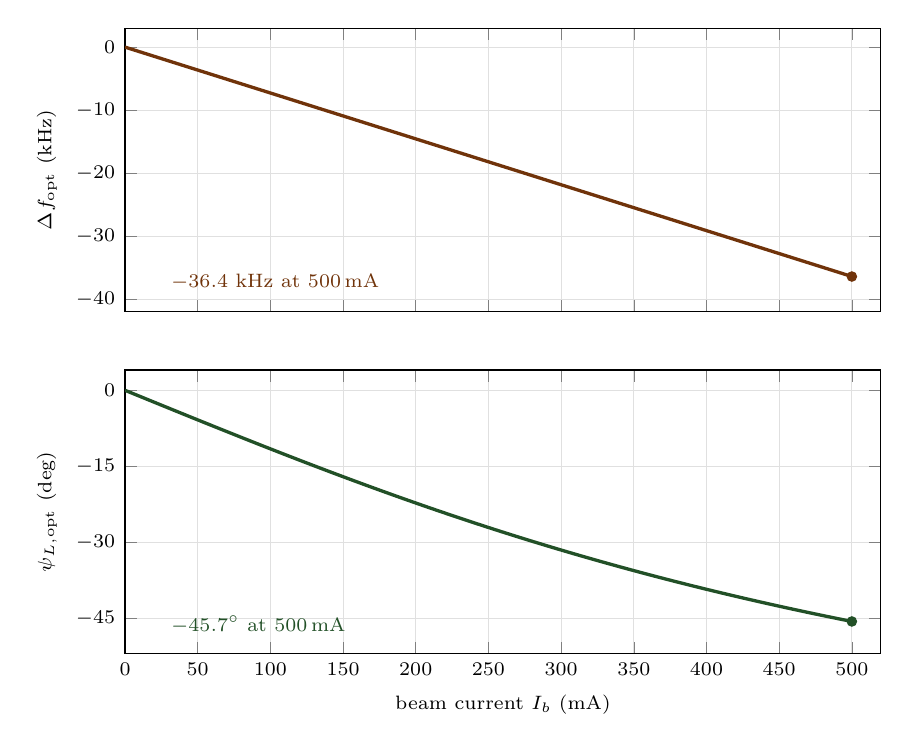
\begin{tikzpicture}[font=\small]
\begin{axis}[
  name=top, width=96mm, height=36mm, scale only axis,
  xmin=0, xmax=520, xticklabels={},
  ymin=-42, ymax=3, ylabel={$\Delta f_\text{opt}$ (kHz)},
  ytick={0,-10,-20,-30,-40},
  grid=both, grid style={draw=black!12},
  tick label style={font=\scriptsize}, label style={font=\scriptsize},
]
\addplot[cPwr!85!black,very thick,domain=0:500,samples=2] {-0.07283*x};
\addplot[only marks,mark=*,mark size=1.7pt,cPwr!85!black] coordinates {(500,-36.42)};
\node[anchor=south west,font=\scriptsize,text=cPwr!85!black] at (axis cs:25,-40)
  {$-36.4$ kHz at \qty{500}{\milli\ampere}};
\end{axis}
\begin{axis}[
  at={(top.below south west)}, anchor=north west, yshift=-5mm,
  width=96mm, height=36mm, scale only axis,
  xmin=0, xmax=520, xlabel={beam current $I_b$ (mA)},
  ymin=-52, ymax=4, ylabel={$\psi_{L,\text{opt}}$ (deg)},
  ytick={0,-15,-30,-45},
  grid=both, grid style={draw=black!12},
  tick label style={font=\scriptsize}, label style={font=\scriptsize},
]
\addplot[cRf!75!black,very thick,domain=0:500,samples=80] {atan(-1.0236*x/500)};
\addplot[only marks,mark=*,mark size=1.7pt,cRf!75!black] coordinates {(500,-45.67)};
\node[anchor=south west,font=\scriptsize,text=cRf!75!black] at (axis cs:25,-50)
  {$-45.7^\circ$ at \qty{500}{\milli\ampere}};
\end{axis}
\end{tikzpicture}
\end{fitpicture}
\caption{Cavity detuning required to cancel the reactive beam loading, as a function of beam current. The frequency offset (top) is linear in current; the loaded detuning angle measured by the tuner loop (bottom) is its arctangent and so compresses at high current.}\label{fig:detuning-vs-current}
\end{figure}

The practical consequence is that the tuner setpoint is never static. It tracks the stored current continuously, and superimposed on that are the slow drifts of D7--D9.

\subsection{What Happens When the Tuner Lags}\label{sec:transient-lag}


\Cref{fig:reflected-power} evaluates \cref{eq:gamma} against cavity tuning for the two extreme beam conditions. The two curves have minima in different places, and that displacement is the whole story of transient matching.

\begin{figure}[tbp]
\centering
\begin{fitpicture}% !TeX root = ../P_rf_physics_and_plant.tex
% Reflected power at the input coupler versus cavity tuning, with and without
% beam.  Plots |Gamma|^2 = [(b-1-a)^2 + (t+b)^2] / [(b+1+a)^2 + (t+b)^2]
% with t = Df/7.44219 kHz  (t = 2 Q0 Df / f0, f0/2Q0 = 7.4422 kHz),
%      beta = 3.78.
%   500 mA:  a = 1.8755, b = 4.8930  ->  beta-1-a = 0.9045, beta+1+a = 6.6555
%   no beam: a = 0,      b = 0       ->  beta-1   = 2.78,   beta+1   = 4.78
% Keep these four constants in step with the cavity table if beta or the
% operating point ever changes.
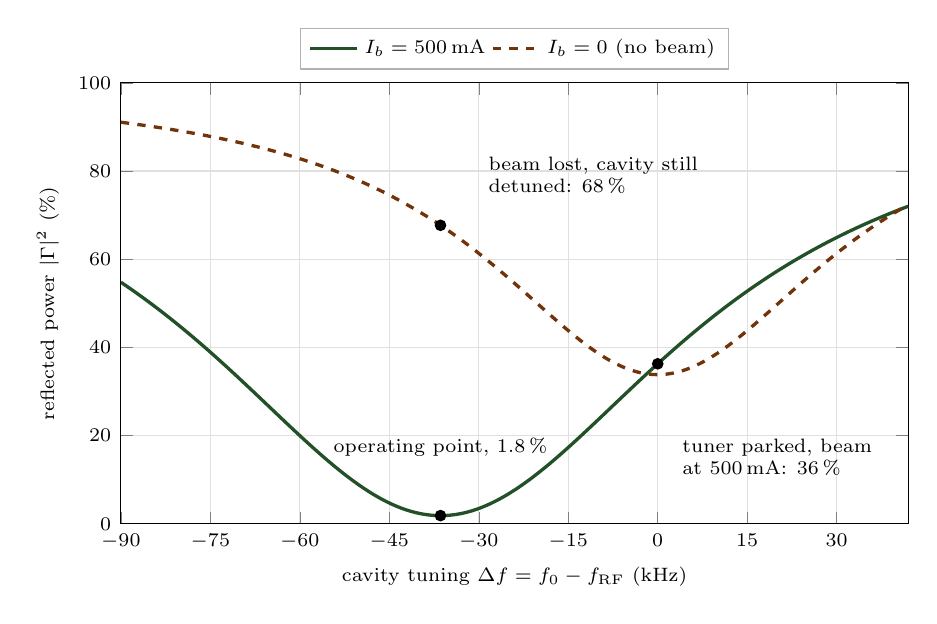
\begin{tikzpicture}[font=\small]
\begin{axis}[
  width=100mm, height=56mm, scale only axis,
  xmin=-90, xmax=42, ymin=0, ymax=100,
  xtick={-90,-75,-60,-45,-30,-15,0,15,30},
  xlabel={cavity tuning $\Delta f = f_0 - f_\text{RF}$ (kHz)},
  ylabel={reflected power $|\Gamma|^2$ (\%)},
  ytick={0,20,40,60,80,100},
  grid=both, grid style={draw=black!12},
  tick label style={font=\scriptsize}, label style={font=\scriptsize},
  legend style={at={(0.5,1.03)},anchor=south,legend columns=2,
                draw=black!30,fill=white,font=\scriptsize},
]
\addplot[cRf!75!black,very thick,domain=-90:42,samples=300]
  {100*(0.9045^2 + (x/7.44219 + 4.8930)^2)/(6.6555^2 + (x/7.44219 + 4.8930)^2)};
\addlegendentry{$I_b=\qty{500}{\milli\ampere}$}
\addplot[cPwr!85!black,very thick,dashed,domain=-90:42,samples=300]
  {100*(2.78^2 + (x/7.44219)^2)/(4.78^2 + (x/7.44219)^2)};
\addlegendentry{$I_b=0$ (no beam)}

% Annotations live in the region under both curves (lower right) or above the
% dashed curve (upper middle); nothing is placed on a curve.
\addplot[only marks,mark=*,mark size=1.9pt,black]
  coordinates {(-36.42,1.85) (0,36.28) (-36.42,67.69)};

\node[anchor=south,font=\scriptsize,align=center] at (axis cs:-36.42,13)
  {operating point, \qty{1.8}{\percent}};
\node[anchor=west,font=\scriptsize,align=left] at (axis cs:2.5,15)
  {tuner parked, beam\\ at \qty{500}{\milli\ampere}: \qty{36}{\percent}};
\node[anchor=west,font=\scriptsize,align=left] at (axis cs:-30,79)
  {beam lost, cavity still\\ detuned: \qty{68}{\percent}};
\end{axis}
\end{tikzpicture}
\end{fitpicture}
\caption{Reflected power at the input coupler against cavity tuning, with and without beam. The minima sit at different detunings, so a cavity tuned for one beam condition is badly mismatched in the other. With no beam the over-coupled cavity cannot be matched at all: the best it can do on resonance is \qty{34}{\percent} reflected.}\label{fig:reflected-power}
\end{figure}

\begin{longtable}[]{@{}Q{\dimexpr 0.2700\linewidth-1.60\tabcolsep\relax}Q{\dimexpr 0.1300\linewidth-1.60\tabcolsep\relax}Q{\dimexpr 0.1000\linewidth-1.60\tabcolsep\relax}Q{\dimexpr 0.1400\linewidth-1.60\tabcolsep\relax}Q{\dimexpr 0.3600\linewidth-1.60\tabcolsep\relax}@{}}
\toprule\noalign{}
Event & Detuning error & \(|\Gamma|^2\) & \(P_\text{fwd}\)/cavity & Consequence \\
\midrule\noalign{}
\endhead
\bottomrule\noalign{}
\endlastfoot
Steady 500 mA, tuner converged & 0 & 1.8\% & 199 kW & The normal operating point \\
Top-off shot, \(\pm\)5 mA & 0.4 kHz & 1.8\% & 199 kW & Below the tuner deadband; invisible \\
Circumference drift, one year & 4 kHz & 2.5\% & 201 kW & Absorbed as a slow migration of the tuner setpoint (D9) \\
Fill 0 \(\rightarrow\) 500 mA, tuner still on resonance & 36.4 kHz & 36\% & 307 kW & \(4 \times 307 = \qty{1.23}{\mega\watt}\), or 82\% of the klystron rating \\
Beam loss 500 \(\rightarrow\) 0 mA, cavity still detuned & 36.4 kHz & 68\% & 211 kW & Only wall loss is delivered, but the circulator load takes 143 kW/cavity \\
No beam, cavity on resonance & 0 & 34\% & 103 kW & The over-coupled floor; cannot be improved without beam \\
\end{longtable}

The two rows that matter operationally are the fill and the beam loss. Both leave the cavity a full half-bandwidth from its matching point, and in both cases a third or more of the forward power goes into the circulator load until the tuner catches up. This is why a fill is done at reduced gap voltage or slowly enough for the tuner to track, and why the circulator load, not the klystron, is the component sized by the transient.

\subsection{Division of Labour: the Direct Loop Holds the Field, the Tuner Restores the Match}\label{sec:transient-roles}


Two loops respond to these transients, and it is worth stating plainly that neither can do the other's job.

\textbf{The direct loop regulates the field, and it is fast.} With \qty{800}{\kilo\hertz} of bandwidth \eqref{eq:fc-max} it corrects a beam-current step within a few microseconds --- far faster than the \qty{4.5}{\micro\second} cavity fill time \eqref{eq:cav-bw}, and faster than any mechanical motion. But it holds \(V_\text{gap}\) by \emph{demanding more generator current}. It does not change \(y_L\): the cavity is exactly as mismatched as before, and the extra forward power is delivered, reflected, and dumped in the circulator load. \textbf{A field-regulation loop cannot reduce reflected power.}

\textbf{The tuner restores the match, and it is slow.} Only the tuner changes \(t\), and it does so at \qtyrange{0.01}{1}{\hertz} through a stepper motor and a mechanical plunger (\cref{sec:loop-tuner,sec:tuner-mech}). It is seven to eight decades slower than the direct loop.

The resulting sequence for any current transient is therefore always the same:

\begin{enumerate}
\def\labelenumi{\arabic{enumi}.}
\tightlist
\item
  The beam current changes, which changes \(a\) and \(b\) essentially instantaneously.
\item
  The direct loop holds \(V_\text{gap}\) through the change. Field amplitude and phase never leave specification.
\item
  The reflected power jumps to the value given by \cref{eq:gamma} at the \emph{old} tuning, and the klystron carries the extra forward power.
\item
  The tuner walks \(t\) back to \(-b\) over seconds, and the reflected power decays to the coupler floor.
\end{enumerate}

\begin{keynote}
\textbf{The separation of timescales is what makes this safe.} Because the direct loop is roughly \(10^6\) times faster than the tuner, the two never interact dynamically --- the tuner sees a cavity whose field is already regulated, and the direct loop sees a detuning that is constant on its own timescale. That is the same bandwidth-separation argument as \cref{eq:bw-sep}, applied to the one pair of loops that share an actuator path. The cost of the separation is that mismatch is corrected slowly, so transient reflected power must be budgeted as a hardware rating rather than regulated away.
\end{keynote}

\begin{keynote}
\textbf{Not covered here}: this analysis is quasi-static in the tuner variable --- it evaluates \cref{eq:gamma} at each tuning, but does not model the tuner's own closed-loop trajectory, its deadband limit cycle, or the coupled dynamics of four independently tuned cavities driven from one klystron. A measured tuner step response and a fill record with synchronised current, forward and reflected power would let those be added; neither is currently in the repository.
\end{keynote}

\section{HVPS Plant Model and Dynamics}\label{sec:hvps}


\subsection{Power Supply Architecture}\label{sec:hvps-arch}


The SPEAR3 klystron HVPS is a PEP-II design: a 12-pulse, primary-side SCR phase-controlled rectifier fed from a 12.47 kV substation feeder \R{21}, \R{22}. Two complete units (SPEAR1 and SPEAR2) are installed; one is energized at a time.

\subsection{HVPS Electrical Parameters}\label{sec:hvps-params}


\begin{longtable}[]{@{}Q{\dimexpr 0.3816\linewidth-1.33\tabcolsep\relax}Q{\dimexpr 0.4474\linewidth-1.33\tabcolsep\relax}Q{\dimexpr 0.1711\linewidth-1.33\tabcolsep\relax}@{}}
\toprule\noalign{}
Parameter & Value & Unit \\
\midrule\noalign{}
\endhead
\bottomrule\noalign{}
\endlastfoot
Input voltage & 12,470 V RMS L-L & 3-phase 60 Hz \\
Output voltage range & 0 to \(-90\) kV & DC \\
Maximum current & 27 A & DC \\
Nominal operating & \(-77\) kV, 22 A & DC \\
Complete-supply rating & 2,750 kVA (12.5 kV at 127 A RMS) & nameplate \\
Voltage regulation & \(< \pm 0.5\%\) & at \(> 65\) kV \\
Voltage ripple & \(< 1\%\) P-P, \(< 0.2\%\) RMS & at \(> 60\) kV \\
Filter inductors (\(L_1, L_2\)) & 0.3 H each & 85 A DC \\
Filter capacitors (\(C\)) & \(8\;\mu\text{F}\) per stage \(\times\) 4 series stages & at 30 kV \\
SCR crowbar arc energy & \(< 5\) J (with), \(< 20\) J (without) & --- \\
\end{longtable}

Ratings are from the HVPS technical specification \R{22} and the original design paper \R{21}. The as-built plant detail behind these numbers --- nameplate, tank contents and stored energy --- is in Doc~L.

\subsection{SCR Phase Control Dynamics}\label{sec:hvps-scr}


\begin{equation}\label{eq:scr-cos}
V_\text{dc} = V_\text{dc,max} \cos\alpha
\end{equation}

The installed firing electronics is an Enerpro FCOG6100 six-pulse board with an FCOAUX60 auxiliary gate-drive board \R{26}; the FCOG1200 named in some upgrade material is the \emph{replacement} part and is not in service. The board\textquotesingle s phase-locked loop free-runs at \(384 \times f_\text{line} = 23.04\) kHz and locks to the AC mains zero crossings, so the delay angle \(\alpha\) is referenced to the line rather than to an internal ramp.

For small-signal control analysis the firing chain is modelled as a single-pole lag:

\begin{equation}\label{eq:enerpro}
H_\text{Enerpro}(s) = \frac{1}{1 + s/\omega_\text{Enerpro}}
\end{equation}

with \(\omega_\text{Enerpro} \approx 415\) rad/s, i.e.\ \(-3\) dB at 66 Hz. That figure comes from the published loop-filter analysis of this firing-circuit family \R{25}, which also gives unity DC gain, a \(+0.81\) dB peak at 60 rad/s and \(-45^\circ\) phase margin at 339 rad/s. The single pole is therefore a simplification --- the measured response peaks slightly, so it is mildly underdamped rather than exactly first order.

\begin{keynote}
\textbf{Small-signal bandwidth and step settling are different numbers, and one does not follow from the other.} The 415 rad/s pole corresponds to \(\tau = 1/\omega_\text{Enerpro} = 2.4\) ms, but a \emph{step} in the SIG HI command settles in \textbf{2--3 AC line cycles}, that is 33--50 ms \R{25}. This is not a contradiction: phase control is a sampled-data process, so a new delay angle can only take effect at the next thyristor firing instant --- one every \(1/(12 f_\text{line}) = 1.39\) ms in the 12-pulse configuration --- and the PLL has to re-acquire after a large disturbance. The 415 rad/s pole shapes the small-signal loop; the 2--3 cycle figure is how long a setpoint change actually takes to arrive.
\end{keynote}

\subsection{PLC Voltage Regulation Loop}\label{sec:hvps-plc}


The SLC-500 PLC implements a first-order IIR filter with scan period \(T = 10\) ms:

\begin{equation}\label{eq:plc-iir}
y[n] = (1-\alpha)\,y[n-1] + \alpha\,x[n]
\end{equation}

with \(\alpha = 0.4\), giving time constant \(\tau = -T/\ln(1-\alpha) \approx 20\) ms \R{27}, \R{23}.

\subsection{Klystron Arc Protection}\label{sec:hvps-arc}


Four mechanisms limit the energy an arc can deposit in the klystron: the SCR crowbar, the star-point bypass, the \(500\;\Omega\) filter isolation resistors and the cable termination inductors. The published PEP-II result is \(< 5\) J to the klystron with the crowbar operating and \(I^2 t < 40\;\text{A}^2\text{s}\) \R{21}.

\begin{keynote}
\textbf{Timing and component caveats}: the crowbar conduction delay is \(\approx 10\;\mu\text{s}\), not sub-microsecond, and primary current interruption takes 4--8 ms; the termination inductors are \textbf{350 \(\mu\)H as built}, not the 200 \(\mu\)H design figure of \R{21}. Both corrections come from the as-built drawing review recorded in Doc~L. These are published design/test results, not an acceptance certification of the installed SPEAR3 units.
\end{keynote}

\subsection{HVPS Dynamic Response Summary}\label{sec:hvps-dynamics}


The elements below are listed fastest first. Each row states the physical time it describes; they are \emph{not} interchangeable, and the equivalent frequency is quoted only where a single-pole or resonant interpretation is meaningful.

\begin{longtable}[]{@{}Q{\dimexpr 0.2600\linewidth-1.50\tabcolsep\relax}Q{\dimexpr 0.2100\linewidth-1.50\tabcolsep\relax}Q{\dimexpr 0.1500\linewidth-1.50\tabcolsep\relax}Q{\dimexpr 0.3800\linewidth-1.50\tabcolsep\relax}@{}}
\toprule\noalign{}
Element & Characteristic time & Equivalent frequency & What the number is \\
\midrule\noalign{}
\endhead
\bottomrule\noalign{}
\endlastfoot
SCR commutation overlap & \(\sim 100\;\mu\text{s}\) & \(\sim 1.6\) kHz & Current transfer between thyristors; not a control-loop limit \\
Output LC filter & \(\sqrt{LC} = 775\;\mu\text{s}\) & \(f_0 \approx 205\) Hz & 0.3 H per leg into the 2 µF net series bank (\cref{sec:hvps-params}); lightly damped resonance \\
12-pulse firing interval & 1.39 ms between firings; \(\approx 0.69\) ms mean transport lag & \(\sim 230\) Hz & Sampling limit of phase control: \(\alpha\) can change only at a firing instant \\
Enerpro small-signal pole & \(\tau = 2.4\) ms & 66 Hz (\(-3\) dB) & \Cref{eq:enerpro}, \(\omega_\text{Enerpro} = 415\) rad/s \R{25} \\
Enerpro step settling & 2--3 line cycles, 33--50 ms & --- & Large-signal settling after a SIG HI step \R{25} \\
PLC digital filter & \(\tau = 20\) ms & \(\sim 8\) Hz & \Cref{eq:plc-iir}, \(\alpha = 0.4\) at a 10 ms scan \\
Open-loop voltage step & \(\approx 50\)--70 ms & \(\sim 3\) Hz & Enerpro settling and PLC filter in series \\
Supervisory update & \(\sim 0.5\) s & \(\sim 1\) Hz & EPICS SNL loop rate (\cref{sec:loop-hvps}) \\
\end{longtable}

\textbf{Nothing in the plant limits the closed HVPS loop.} The loop is closed in EPICS software at roughly 2 Hz (\cref{sec:loop-hvps}), so its \(\sim 1\) Hz bandwidth is more than an order of magnitude slower than the slowest plant element above. The HVPS is therefore a quasi-static actuator as far as the RF control system is concerned --- which is precisely why HVPS ripple (D5, \cref{sec:d5}) must be rejected downstream by the ripple loop and by the direct loop, and cannot be regulated away by the HVPS controller itself.

\begin{center}\rule{0.5\linewidth}{0.5pt}\end{center}

\section{Tuner Mechanics and Resonant Frequency Control}\label{sec:tuner-mech}


\subsection{Cavity Tuner Physical Description}\label{sec:tuner-hw}


Mechanism and motor data are from the tuner documentation set \R{29}--\R{33}; the 2023 mechanical inspection findings are in \R{28}.

\begin{longtable}[]{@{}Q{\dimexpr 0.3143\linewidth-1.00\tabcolsep\relax}Q{\dimexpr 0.6857\linewidth-1.00\tabcolsep\relax}@{}}
\toprule\noalign{}
Parameter & Value \\
\midrule\noalign{}
\endhead
\bottomrule\noalign{}
\endlastfoot
Motor & Superior Electric Slo-Syn M093-FC11 (NEMA 34D) \\
Drive mechanism & Worm gear (self-locking) \\
Tuning range & \(\sim \pm 200\) kHz \\
Step resolution & \(\sim 1\) Hz/step \\
Distance per microstep & \(3.175\;\mu\text{m}\) (legacy), \(0.05\;\mu\text{m}\) (Galil) \\
\end{longtable}

\subsection{Tuning Physics}\label{sec:tuner-physics}


The cavity resonant frequency is a smooth, monotonic function of plunger insertion depth over the working range. It is represented in the control software by the cubic-plus-quadratic-voltage model of \cref{eq:tuner-poly}, whose coefficients \(p_0 \ldots p_3\) and \(t_1\) are obtained by the frequency/detuning calibration described in \cref{sec:cal-freq}.

The cavity body also drifts with copper temperature. The first-principles coefficient for an uncooled body is \(-7.9\) kHz/°C \eqref{eq:cav-thermal}; with the regulated water-cooling circuit in service the \emph{observed} drift referred to the cavity cooling-water setpoint is roughly an order of magnitude smaller, \(\sim -1\) kHz/°C. The tuner loop of \cref{sec:loop-tuner} absorbs both.

\begin{center}\rule{0.5\linewidth}{0.5pt}\end{center}

\section{Performance Requirements and Verification}\label{sec:performance}


\subsection{Disturbance Rejection Summary}\label{sec:perf-rejection}


\begin{longtable}[]{@{}Q{\dimexpr 0.2414\linewidth-1.60\tabcolsep\relax}Q{\dimexpr 0.2644\linewidth-1.60\tabcolsep\relax}Q{\dimexpr 0.2069\linewidth-1.60\tabcolsep\relax}Q{\dimexpr 0.1494\linewidth-1.60\tabcolsep\relax}Q{\dimexpr 0.1379\linewidth-1.60\tabcolsep\relax}@{}}
\toprule\noalign{}
Disturbance & Frequency & Open-Loop Impact & Rejection & Residual \\
\midrule\noalign{}
\endhead
\bottomrule\noalign{}
\endlastfoot
Beam loading (D1--D2) & DC--100 kHz & Unstable & \(\sim 40\) dB & Stable \\
Robinson (D3) & \(\sim 10\) kHz \eqref{eq:nus} & Exponential growth & \(\sim 40\) dB & \(\ll 1/\tau_s\) \\
HVPS ripple (D5) & 360--2000 Hz & \(\sim 1\%\) phase & \(\sim 40\) dB & \(< 0.01\%\) \\
Thermal drift (D8) & \(< 0.01\) Hz & \(\sim 100\) Hz/hr & Tuner tracks & \(< 1\) Hz \\
Klystron gain (D6) & 0.01--1 Hz & \(\sim 7\) dB var. & Gain tracking & \(< 0.5\) dB \\
\end{longtable}

\subsection{LLRF9 Commissioning Results}\label{sec:perf-llrf9}


From \R{4}: the LLRF9 controller \W{4} achieves an improved noise floor relative to the legacy VXI system at 500 mA. Overall amplitude stability \(< 0.05\%\) RMS and phase stability \(< 0.05^\circ\) RMS --- both better than the requirements of \cref{sec:field-stability}.

\subsection{Performance Margins}\label{sec:perf-margins}


\begin{longtable}[]{@{}Q{\dimexpr 0.2500\linewidth-1.50\tabcolsep\relax}Q{\dimexpr 0.1711\linewidth-1.50\tabcolsep\relax}Q{\dimexpr 0.3684\linewidth-1.50\tabcolsep\relax}Q{\dimexpr 0.2105\linewidth-1.50\tabcolsep\relax}@{}}
\toprule\noalign{}
Parameter & Capacity & Typical & Margin \\
\midrule\noalign{}
\endhead
\bottomrule\noalign{}
\endlastfoot
Klystron power & 1.5 MW & \(\sim 782\) kW (\(4 \times 195.6\)) & \(\sim 48\%\) \\
HVPS voltage & 90 kV & \(\sim 72\)--\(77\) kV & \(\sim 15\%\) \\
Gap voltage/cavity & 1 MV & \(\sim 712\) kV & \(\sim 40\%\) \\
Direct loop BW & \(\sim 930\) kHz & \(\sim 800\) kHz & \(\sim 16\%\) \\
Impedance reduction & \(\sim 40\) dB & Required \(\sim 30\) dB & \(> 10\) dB margin \\
\end{longtable}

\subsection{Calibration Data}\label{sec:cal}


Calibration establishes the numerical relationships between raw hardware signals (ADC counts, DAC counts, detector voltages) and physical quantities (kV, kW, degrees, Hz). It is essential for closing all feedback loops accurately. This section is a high-level summary; the measured coefficient tables themselves live with the calibration data files \R{38}, \R{39}.

\subsubsection{Calibration Sequence Overview}\label{sec:cal-sequence}


The master calibration is executed by \texttt{rf\_calib.st,v} (3,345 lines, 28 states including setup and abort handling). It runs as an EPICS SNL program and requires the station to be OFF (no RF power). The sequence progresses through the following phases:

\begin{longtable}[]{@{}Q{\dimexpr 0.1382\linewidth-1.33\tabcolsep\relax}Q{\dimexpr 0.3889\linewidth-1.33\tabcolsep\relax}Q{\dimexpr 0.4730\linewidth-1.33\tabcolsep\relax}@{}}
\toprule\noalign{}
Phase & States & What It Does \\
\midrule\noalign{}
\endhead
\bottomrule\noalign{}
\endlastfoot
\textbf{Initialization} & Startup, CombCheck, Setup & Registers with RFP module, verifies hardware, sets known baseline \\
\textbf{Zero all multipliers} & ZeroCavMults, ZeroDirMults, ZeroCombMults & Writes zero to all I/Q modulator DACs --- establishes the "no signal" baseline for offset measurement \\
\textbf{Combiner calibration} & Combiner & Calibrates the 4 cavity combining modulators: measures each probe independently, adjusts I/Q matrix for accurate vector sum \\
\textbf{Direct loop calibration} & Direct, SummingNodeI/Q, GainStageI/Q & Characterizes direct loop gain stages and summing node offsets. I and Q channels measured independently to resolve cross-coupling \\
\textbf{Klystron chain} & ZeroKlysMults, DiffNodeOffsets, KlysStage, CompStage, CombStage, KlysDemod & Calibrates klystron forward path: drive modulator offsets, klystron gain, compensator stages, demodulator phase alignment \\
\textbf{Tuner \& modulator} & TuneStage, NullModulator & Calibrates tune-mode drive path; nulls RF modulator output (zero DAC → zero RF) \\
\textbf{Completion} & Finish/Done or Abort/Abend & Restores operational configuration, reports success/failure \\
\end{longtable}

Each state includes retry logic (\texttt{NUM\_TRIES} iterations), severity checking on PV readbacks, and abort handling. The entire sequence takes \textasciitilde2--5 minutes.

\subsubsection{Drive Amplitude Calibration}\label{sec:cal-drive}


Establishes the mapping from DAC counts to klystron input drive power. Data files: \texttt{driveAmpCalibration.\allowbreak{}xlsx}, \texttt{klystronCouplerDriveAmpCalibrations.\allowbreak{}xlsx}.

The key relationship is the \textbf{drive conversion constant} \(D_\text{conv}\) (counts/kV), computed by \texttt{subIQampl2conv}:

\begin{equation}\label{eq:dconv}
D_\text{conv} = \frac{A_\text{ref}}{V_\text{gap} \cdot (1 + G_\text{loop})}
\end{equation}

where \(A_\text{ref}\) is the reference amplitude (counts), \(V_\text{gap}\) is the measured gap voltage (kV), and \(G_\text{loop}\) is the feedback loop gain. This constant is used by the DAC loop \eqref{eq:dac-law} and recomputed whenever the operating point changes.

\subsubsection{Power Measurement Calibration}\label{sec:cal-power}


Maps RF detector voltages to physical power levels. Data files: \texttt{reflectedPowerCalibrations.\allowbreak{}xlsx}, \texttt{pulsarCouplerCalibration2049.\allowbreak{}xlsx}.

The \textbf{RF detector conversion loss} measured during calibration (\texttt{subIQampl2loss}):

\begin{equation}\label{eq:det-loss}
L_\text{det} = 20 \cdot \log_{10}\!\left(\frac{E_\text{conv} \cdot \sqrt{P_\text{cal}}}{A_\text{det}}\right) \;\text{dB}
\end{equation}

where \(E_\text{conv} = 0.31623\) (power conversion constant), \(P_\text{cal}\) is calibration power (mW), and \(A_\text{det}\) is measured detector amplitude (V). Accounts for cable attenuation, coupler directivity, and detector nonlinearity.

The \textbf{coupling factor} (VSWR-based, \texttt{subIQamplCplg}):

\begin{equation}\label{eq:beta-meas}
\beta_\text{meas} = \frac{1 + r}{1 - r}, \qquad r = \frac{A_\text{refl}}{A_\text{fwd}}
\end{equation}

\subsubsection{Frequency and Detuning Calibration}\label{sec:cal-freq}


Maps tuner motor position to cavity resonant frequency offset. The polynomial model \eqref{eq:tuner-poly} is fitted from measured data: the tuner is stepped across its range and the resonant frequency measured at each position. Calibration coefficients \(p_0, \ldots, p_3\) and temperature coefficient \(t_1\) are stored in EPICS PVs.

\subsubsection{Tuner Mode DAC Calibration}\label{sec:cal-tunemode}


Data file: \texttt{tuneModeDacCalibration.\allowbreak{}xlsx}. Establishes DAC counts-to-drive-power for the \texttt{STATION\_TUNE} state (low-power cavity conditioning). Separate from operational drive calibration (\cref{sec:cal-drive}) because the operating point differs.

\subsubsection{Signal Routing and Patch Panel}\label{sec:cal-routing}


Data file: \texttt{b132R11PatchPanel.\allowbreak{}xlsx}. Documents physical signal routing in Building 132 R11: cable lengths, attenuation values, connector types, and signal naming. Essential for verifying the delay budget (\cref{sec:delay-budget}) and signal levels.

\begin{keynote}
\textbf{Upgrade note}: Many calibrations will need adaptation for the LLRF9 system (different ADC/DAC ranges, signal levels, processing gains). The polynomial frequency model \eqref{eq:tuner-poly} and combiner matrix calibration are expected to transfer; drive and power detector calibrations require new measurements.
\end{keynote}

\begin{center}\rule{0.5\linewidth}{0.5pt}\end{center}

\appendix

\section{SPEAR3 RF System Parameter Table}\label{app:params}


\subsection{Storage Ring Parameters}\label{sec:a1-ring}


\begin{longtable}[]{@{}Q{\dimexpr 0.3333\linewidth-1.60\tabcolsep\relax}Q{\dimexpr 0.1222\linewidth-1.60\tabcolsep\relax}Q{\dimexpr 0.2000\linewidth-1.60\tabcolsep\relax}Q{\dimexpr 0.0444\linewidth-1.60\tabcolsep\relax}Q{\dimexpr 0.3000\linewidth-1.60\tabcolsep\relax}@{}}
\toprule\noalign{}
Parameter & Symbol & Value & Unit & Source \\
\midrule\noalign{}
\endhead
\bottomrule\noalign{}
\endlastfoot
Beam energy & \(E_0\) & 3.0 & GeV & \R{1} \\
Beam current & \(I_b\) & 500 & mA & \R{1} \\
Circumference & \(C\) & 234.14 & m & \R{2} \\
Revolution frequency & \(f_\text{rev}\) & 1.2804 & MHz & Derived \\
Harmonic number & \(h\) & 372 & --- & \R{1} \\
RF frequency & \(f_\text{RF}\) & 476.3 & MHz & \R{4} \\
Momentum compaction & \(\alpha_c\) & \(1.18 \times 10^{-3}\) & --- & \R{2} \\
Energy loss per turn & \(U_0\) & 1.02 & MeV & Operational (current IDs) \\
Total RF voltage (design) & \(V_\text{RF}\) & 3.2 & MV & \R{1} \R{3} \\
Total RF voltage (operational) & \(V_\text{RF}\) & \textasciitilde2.85 & MV & \R{4} \R{5} \\
Synchronous phase & \(\phi_s\) & 69.0 & deg & \cref{eq:phis-eval} (\(\cos\) convention) \\
Synchrotron tune & \(\nu_s\) & \textasciitilde0.008 & --- & \cref{eq:nus}; \R{1} \\
Synchrotron frequency & \(f_s\) & \textasciitilde10.1 & kHz & \cref{eq:nus} \\
Long. radiation damping time & \(\tau_s\) & 2.87 & ms & \R{1} \\
Trans. radiation damping time & \(\tau_{x,y}\) & 4.24, 5.14 & ms & \R{1} \\
\end{longtable}

\subsection{Cavity Parameters (Per Cavity)}\label{sec:a2-cavity}


\begin{longtable}[]{@{}Q{\dimexpr 0.3585\linewidth-1.60\tabcolsep\relax}Q{\dimexpr 0.2075\linewidth-1.60\tabcolsep\relax}Q{\dimexpr 0.1321\linewidth-1.60\tabcolsep\relax}Q{\dimexpr 0.0566\linewidth-1.60\tabcolsep\relax}Q{\dimexpr 0.2453\linewidth-1.60\tabcolsep\relax}@{}}
\toprule\noalign{}
Parameter & Symbol & Value & Unit & Source \\
\midrule\noalign{}
\endhead
\bottomrule\noalign{}
\endlastfoot
Resonant frequency & \(f_0\) & ≈ 476.3 & MHz & \R{6} \\
Shunt impedance (linac) & \(R_s\) & 3.73 & MΩ & \R{6} \\
\(R/Q\) & \(R/Q\) & \textasciitilde116 & Ω & \R{7} \\
Unloaded Q & \(Q_0\) & 32,000 & --- & \R{6} \\
Loaded Q & \(Q_L\) & 6,700 & --- & Derived from \(\beta = 3.78\) \\
Coupling coefficient (this doc) & \(\beta\) & 3.78 & --- & Derived \\
Coupling coefficient (Schwarz actual) & \(\beta\) & 3.72 & --- & \R{6} \\
Coupling coefficient (Schwarz optimum) & \(\beta\) & 3.84 & --- & \R{6} \\
Cavity half-bandwidth & \(\Delta f_{1/2}\) & 35.5 & kHz & Derived \\
Operational gap voltage & \(V_\text{gap}\) & \textasciitilde712 & kV & \R{5} \\
Beam-induced voltage & \(V_{b,\text{res}}\) & 0.78 & MV/cav & \cref{eq:vb-res} \\
Optimum detuning angle (loaded) & \(\psi_{L,\text{opt}}\) & \(\approx -45.7\) & deg & \cref{eq:psi-opt-eval} \\
Optimum frequency detuning & \(\Delta f_\text{opt}\) & \(\approx -36.4\) & kHz & \cref{eq:df-opt} \\
Cavity wall losses & \(P_\text{wall}\) & \textasciitilde68.1 & kW/cav & \cref{eq:pwall} \\
Beam power per cavity & \(P_\text{beam}/n_\text{cav}\) & \textasciitilde127.5 & kW/cav & \cref{eq:pbeam} \\
Generator power per cavity & \(P_\text{gen/cav}\) & \textasciitilde196 & kW & \cref{eq:pgen-eval} \\
Total RF power (4 cav) & \(P_\text{gen,tot}\) & \textasciitilde782 & kW & \(4 \times P_\text{gen/cav}\) \\
\end{longtable}

\subsection{Klystron Parameters}\label{sec:a3-klystron}


\begin{longtable}[]{@{}Q{\dimexpr 0.2453\linewidth-1.50\tabcolsep\relax}Q{\dimexpr 0.3962\linewidth-1.50\tabcolsep\relax}Q{\dimexpr 0.2453\linewidth-1.50\tabcolsep\relax}Q{\dimexpr 0.1132\linewidth-1.50\tabcolsep\relax}@{}}
\toprule\noalign{}
Parameter & Value & Unit & Source \\
\midrule\noalign{}
\endhead
\bottomrule\noalign{}
\endlastfoot
Type & Marconi/CPI K3512S & --- & \R{1} \\
Maximum power & 1.5 MW CW & --- & \R{1} \\
Gain & 43 dB min & --- & \R{1} \\
Bandwidth & 5 MHz (\(-3\) dB) & --- & \R{1} \\
Group delay & \(< 150\) ns & --- & \R{1} \\
Drive power & \(\sim 29\) W & --- & \R{5} \\
Perveance \(K\) & \(\sim 1.0 \times 10^{-6}\) & \(\text{A/V}^{3/2}\) & \cref{sec:klystron} \\
\end{longtable}

\subsection{Feedback Loop Parameters}\label{sec:a4-loops}


\begin{longtable}[]{@{}Q{\dimexpr 0.1613\linewidth-1.60\tabcolsep\relax}Q{\dimexpr 0.2903\linewidth-1.60\tabcolsep\relax}Q{\dimexpr 0.2097\linewidth-1.60\tabcolsep\relax}Q{\dimexpr 0.2419\linewidth-1.60\tabcolsep\relax}Q{\dimexpr 0.0968\linewidth-1.60\tabcolsep\relax}@{}}
\toprule\noalign{}
Loop & Bandwidth & SPEAR3 Status & Addresses & Source \\
\midrule\noalign{}
\endhead
\bottomrule\noalign{}
\endlastfoot
Direct & \(\sim 800\) kHz & Active & D1--D4 & \R{14} \\
Comb & 2 MHz & Not used & D4 & \R{14} \\
Ripple & \(\sim 300\) Hz & Active & D5 & \R{14} \\
Gap FF & 100 Hz & Not used & D2 & \R{14} \\
HVPS & \(\sim 1\) Hz & Active & D6 & \R{14} \\
Tuner & \(\sim 0.01\)--\(1\) Hz & Active & D7, D8, D9 & \R{14} \\
DAC & \(\sim 0.1\) Hz & Active & Amplitude drift & \R{14} \\
LFB Woofer & 1 MHz & Not used & D2, D4 & \R{15}, \R{41} \\
\end{longtable}

\begin{center}\rule{0.5\linewidth}{0.5pt}\end{center}

\section{Source Document Reference Index}\label{app:refs}


\subsection{Published Papers}\label{sec:b1-papers}


The \textbf{Web} column links to the external locator listed in \cref{sec:b4-web}.

\begin{longtable}[]{@{}Q{\dimexpr 0.06\linewidth-1.33\tabcolsep\relax}Q{\dimexpr 0.84\linewidth-1.33\tabcolsep\relax}Q{\dimexpr 0.10\linewidth-1.33\tabcolsep\relax}@{}}
\toprule\noalign{}
Ref & Citation & Web \\
\midrule\noalign{}
\endhead
\bottomrule\noalign{}
\endlastfoot
\RDEF{1} & McIntosh, P. et al., "The SPEAR3 RF System," SLAC-PUB-10983, EPAC 2004 & \W{1}, \W{2} \\
\RDEF{2} & Hettel, R. et al., "Design of the SPEAR 3 Light Source," PAC 1999 & --- \\
\RDEF{7} & Rimmer, R.A. et al., "RF Cavity Development for the PEP-II B Factory," LBL-33360, 1992 & --- \\
\RDEF{11} & Gamp, A., "Beam-Cavity Interaction," CAS 2011, arXiv:1112.3203 & \W{3} \\
\RDEF{12} & Wilson, P.B., "Fundamental-Mode RF Design," SLAC-PUB-6062, 1993 & --- \\
\RDEF{13} & Boussard, D., "Control of Cavities with High Beam Loading," PAC 1985 & \W{5} \\
\RDEF{15} & Corredoura, P., "Architecture and Performance of the PEP-II Low-Level RF System," SLAC-PUB-8124, PAC 1999 & --- \\
\RDEF{16} & Robinson, K.W., "Stability of Beam in RF Systems," CEA-CEAL-1010, 1964 & --- \\
\RDEF{17} & Rimmer, R.A. et al., "Comparison of Calculated, Measured, and Beam Sampled Impedances," PRSTAB 3, 102001, 2000 & --- \\
\RDEF{21} & Cassel, R. and Nguyen, M.N., "A Unique Power Supply for the PEP II Klystron," SLAC-PUB-7591, PAC 1997. Repository copy: \fpath{hvps/architecture/originalDocuments/slac-pub-7591.pdf} & --- \\
\RDEF{25} & Bourbeau, E.J., "Application of PLL Techniques to SCR Drives," IEEE 1983 & --- \\
\RDEF{41} & Fox, J.D. et al., "Multi-Bunch Longitudinal Feedback --- Woofer and Kicker Architecture," PEP-II LFB system design note & --- \\
\end{longtable}

\subsection{Textbooks}\label{sec:b2-books}


\begin{longtable}[]{@{}Q{\dimexpr 0.0526\linewidth-1.00\tabcolsep\relax}Q{\dimexpr 0.9474\linewidth-1.00\tabcolsep\relax}@{}}
\toprule\noalign{}
Ref & Citation \\
\midrule\noalign{}
\endhead
\bottomrule\noalign{}
\endlastfoot
\RDEF{3} & SSRL SPEAR Storage Ring Parameters, \url{https://www-ssrl.slac.stanford.edu/accphy/spear_parameters.html} (last updated 26 Apr 2002, H.-D. Nuhn) \\
\RDEF{10} & Wiedemann, H., \emph{Particle Accelerator Physics}, 4th ed., Springer, 2015 \\
\RDEF{18} & Analog Devices AD834 datasheet \\
\RDEF{40} & Åström, K.J. and Murray, R.M., \emph{Feedback Systems: An Introduction for Scientists and Engineers}, 2nd ed., Princeton, 2021 (Ch. 12, loop interaction) \\
\end{longtable}

\subsection{Repository Documents}\label{sec:b3-repo}


\begin{longtable}[]{@{}Q{\dimexpr 0.0591\linewidth-1.33\tabcolsep\relax}Q{\dimexpr 0.3317\linewidth-1.33\tabcolsep\relax}Q{\dimexpr 0.6092\linewidth-1.33\tabcolsep\relax}@{}}
\toprule\noalign{}
Ref & Document & Path \\
\midrule\noalign{}
\endhead
\bottomrule\noalign{}
\endlastfoot
\RDEF{4} & LLRF9 Commissioning Tests & \texttt{llrf/\allowbreak{}tests/\allowbreak{}llrf9Tests.\allowbreak{}pdf} \\
\RDEF{5} & System Design Report & \texttt{Designs/\allowbreak{}tex/\allowbreak{}doc0-\allowbreak{}system-\allowbreak{}design/\allowbreak{}0\_\allowbreak{}system\_\allowbreak{}design\_\allowbreak{}report.\allowbreak{}pdf} \\
\RDEF{6} & RF System Description (Schwarz) & \texttt{llrf/\allowbreak{}documentation/\allowbreak{}legacyArchitecture/\allowbreak{}ps3403305100.\allowbreak{}pdf} \\
\RDEF{14} & Feedback Loop Description (Schwarz, PS-340-330-52-R0) & \texttt{llrf/\allowbreak{}documentation/\allowbreak{}legacyArchitecture/\allowbreak{}feedbackLoopDescriptionps3403305200.\allowbreak{}pdf} \\
\RDEF{22} & HVPS Technical Spec (PS-341-360-01-R2) & \texttt{hvps/\allowbreak{}architecture/\allowbreak{}originalDocuments/\allowbreak{}ps3413600102.\allowbreak{}pdf} \\
\RDEF{23} & HVPS Simulation Config & \texttt{hvps/\allowbreak{}simulation/\allowbreak{}hvps\_\allowbreak{}sim/\allowbreak{}config.\allowbreak{}py} \\
\RDEF{26} & Enerpro firing-board schematics and manuals (FCOG6100 in service, FCOG1200 for the upgrade) & \texttt{hvps/\allowbreak{}controls/\allowbreak{}enerpro/\allowbreak{}enerproDocuments/} \\
\RDEF{27} & Cassel PLC Code & \texttt{hvps/\allowbreak{}documentation/\allowbreak{}plc/\allowbreak{}CasselPLCCode.\allowbreak{}pdf} \\
\RDEF{28} & Cavity Tuner Inspection Report, 13 June 2023 & \texttt{llrf/\allowbreak{}tuners/\allowbreak{}cavityTunerInspections20230613.\allowbreak{}docx} \\
\RDEF{29} & Tuner mechanical design paper, PAC 1997 & \texttt{llrf/\allowbreak{}tuners/\allowbreak{}tunerDesignPac97HDS8P030.\allowbreak{}PDF} \\
\RDEF{30} & Superior Electric SLO-SYN stepper motor data & \texttt{llrf/\allowbreak{}tuners/\allowbreak{}SLO-\allowbreak{}SYN.\allowbreak{}pdf} \\
\RDEF{31} & SLO-SYN MD808 Stepper Drive Manual & \texttt{llrf/\allowbreak{}tuners/\allowbreak{}SLO-\allowbreak{}SYN\_\allowbreak{}MD808\_\allowbreak{}Stepper\_\allowbreak{}Drive\_\allowbreak{}Manual.\allowbreak{}pdf} \\
\RDEF{32} & SLO-SYN SS2000MD4M Step Drive / Translator Manual & \texttt{llrf/\allowbreak{}tuners/\allowbreak{}SLO-\allowbreak{}SYN\_\allowbreak{}SS2000MD4M\_\allowbreak{}Step\_\allowbreak{}Drive\_\allowbreak{}Translator\_\allowbreak{}Manual.\allowbreak{}pdf} \\
\RDEF{33} & Superior Electric stepper catalogue (legacy) & \texttt{llrf/\allowbreak{}tuners/\allowbreak{}Old\ Stepper\ Catalog\_\allowbreak{}Superior\ Electric\_\allowbreak{}0.\allowbreak{}pdf} \\
\RDEF{34} & Tuner Loop Source Code & \texttt{spear-\allowbreak{}rf-\allowbreak{}code-\allowbreak{}legacy/\allowbreak{}rfApp/\allowbreak{}src/\allowbreak{}seq/\allowbreak{}rf\_\allowbreak{}tuner\_\allowbreak{}loop.\allowbreak{}st,\allowbreak{}v} \\
\RDEF{35} & Galil Commissioning Notes & \texttt{llrf/\allowbreak{}tuners/\allowbreak{}galil/\allowbreak{}GalilCommissioning.\allowbreak{}docx} \\
\RDEF{36} & DSP Ripple Firmware & \texttt{spear-\allowbreak{}rf-\allowbreak{}code-\allowbreak{}legacy/\allowbreak{}rfApp/\allowbreak{}src/\allowbreak{}dsp/\allowbreak{}rfpDsp/\allowbreak{}ripple.\allowbreak{}s,\allowbreak{}v} \\
\RDEF{38} & RF Calibration Data & \texttt{llrf/\allowbreak{}calibrations/\allowbreak{}*.\allowbreak{}xlsx} \\
\RDEF{39} & RF Document Index & \texttt{llrf/\allowbreak{}documentation/\allowbreak{}RfSystemDocumentIndexR3.\allowbreak{}xlsx} \\
\end{longtable}

\subsection{External Web References}\label{sec:b4-web}


\begin{longtable}[]{@{}Q{\dimexpr 0.0400\linewidth-1.33\tabcolsep\relax}Q{\dimexpr 0.6034\linewidth-1.33\tabcolsep\relax}Q{\dimexpr 0.3566\linewidth-1.33\tabcolsep\relax}@{}}
\toprule\noalign{}
Ref & URL & Content \\
\midrule\noalign{}
\endhead
\bottomrule\noalign{}
\endlastfoot
\WDEF{1} & \url{https://inspirehep.net/files/945e7ff73cc428af4c018fd1bdb6afa7} & \R{1} McIntosh, EPAC 2004 \\
\WDEF{2} & \url{https://www.osti.gov/biblio/839730} & \R{1} OSTI record, SLAC-PUB-10983 \\
\WDEF{3} & \url{https://export.arxiv.org/pdf/1112.3203v1.pdf} & \R{11} Gamp, CAS 2011 \\
\WDEF{4} & \url{https://www.dimtel.com/products/llrf9} & Dimtel LLRF9 product page (upgrade controller) \\
\WDEF{5} & \url{https://proceedings.jacow.org/p85/PDF/PAC1985_1852.PDF} & \R{13} Boussard, PAC 1985 \\
\end{longtable}

\begin{center}\rule{0.5\linewidth}{0.5pt}\end{center}

\section{Symbol and Notation Conventions}\label{app:symbols}


\subsection{Cavity and Beam Parameters}\label{sec:c1-symbols}


\begin{longtable}[]{@{}Q{\dimexpr 0.1413\linewidth-1.50\tabcolsep\relax}Q{\dimexpr 0.6848\linewidth-1.50\tabcolsep\relax}Q{\dimexpr 0.0761\linewidth-1.50\tabcolsep\relax}Q{\dimexpr 0.0978\linewidth-1.50\tabcolsep\relax}@{}}
\toprule\noalign{}
Symbol & Definition & Unit & First Ref \\
\midrule\noalign{}
\endhead
\bottomrule\noalign{}
\endlastfoot
\(f_0\) & Cavity resonant frequency & MHz & \cref{eq:cav-imp} \\
\(f_\text{RF}\) & RF operating frequency (\(= h \cdot f_\text{rev}\)) & MHz & \cref{sec:ring-params} \\
\(f_\text{rev}\) & Revolution frequency & MHz & \cref{sec:ring-params} \\
\(\omega_0\) & Angular resonant frequency (\(= 2\pi f_0\)) & rad/s & \cref{eq:cav-imp} \\
\(\omega_{1/2}\) & Cavity half-bandwidth (\(= \omega_0 / 2Q_L = 2\pi \times 35.5\) kHz) & rad/s & \cref{eq:cav-tf} \\
\(\Delta f_{1/2}\) & Cavity half-bandwidth (linear frequency) & kHz & \cref{eq:cav-bw} \\
\(Q_0\) & Unloaded quality factor & --- & \cref{sec:cavity-circuit} \\
\(Q_L\) & Loaded quality factor & --- & \cref{sec:cavity-circuit} \\
\(Q_\text{ext}\) & External quality factor (coupling port) & --- & \cref{sec:cavity-circuit} \\
\(\beta\) & Coupling coefficient (\(= Q_0/Q_\text{ext}\)) & --- & \cref{sec:cavity-circuit} \\
\(R_s\) & Shunt impedance (circuit convention: \(V^2/2P\)) & MΩ & \cref{sec:cavity-circuit} \\
\(R_a\) & Shunt impedance (accelerator convention: \(V^2/P = 2R_s\)) & MΩ & \cref{sec:c2-symbols} \\
\(V_\text{gap}\) & Gap voltage per cavity & kV & \cref{sec:cavity-circuit} \\
\(V_\text{RF}\) & Total RF voltage (\(= n_\text{cav} \times V_\text{gap}\)) & MV & \cref{sec:beam-loading} \\
\(I_b\) & DC beam current & A & \cref{sec:beam-loading} \\
\(I_{b1}\) & Fundamental RF component of the bunched beam current (\(= 2I_b\)) & A & \cref{eq:vb-res} \\
\(V_{b,\text{res}}\) & Beam-induced voltage at resonance (\(= I_b R_s\)) & MV & \cref{eq:vb-res} \\
\(\phi_s\) & Synchronous phase angle (from voltage crest) & degrees & \cref{eq:phis} \\
\(\psi\) & Detuning angle & degrees & \cref{eq:psi-opt} \\
\(\psi_0,\ \psi_L\) & Detuning angle referred to the unloaded / loaded bandwidth (\(\tan\psi_L = \tan\psi_0/(1+\beta)\)) & degrees & \cref{eq:psi-opt-eval} \\
\(\psi_\text{opt}\) & Optimum detuning angle & degrees & \cref{eq:psi-opt-eval} \\
\(a\) & Beam loading parameter, real part (\(= P_\text{beam}/P_\text{wall}\)) & --- & \cref{eq:blparams} \\
\(b\) & Beam loading parameter, reactive part & --- & \cref{eq:blparams} \\
\(t\) & Normalised detuning (\(= \tan\psi_0 = 2Q_0\Delta f/f_0\)) & --- & \cref{eq:blparams} \\
\(\Gamma\) & Voltage reflection coefficient at the input coupler & --- & \cref{eq:gamma} \\
\(\beta_\text{opt}\) & Coupling that matches the loaded cavity (\(= 1+a\)) & --- & \cref{eq:gamma-min} \\
\(\Delta f\) & Frequency detuning (\(= f_0 - f_\text{RF}\)) & kHz & \cref{eq:df-opt} \\
\(\Delta\omega\) & Angular frequency offset from RF & rad/s & \cref{eq:cav-imp} \\
\(U_0\) & Energy loss per turn (synchrotron radiation) & MeV & \cref{sec:ring-params} \\
\(h\) & Harmonic number (\(= f_\text{RF}/f_\text{rev}\)) & --- & \cref{sec:ring-params} \\
\(\alpha_c\) & Momentum compaction factor & --- & \cref{eq:nus} \\
\(\nu_s\) & Synchrotron tune (\(= f_s/f_\text{rev}\)) & --- & \cref{eq:nus} \\
\(f_s\) & Synchrotron frequency & kHz & \cref{eq:nus} \\
\(E_0\) & Beam energy (3.0 GeV; expressed in MeV when used with \(V_\text{RF}\) in MV) & GeV & \cref{eq:nus} \\
\(n_\text{cav}\) & Number of cavities & --- & \cref{eq:pgen} \\
\end{longtable}

\subsection{Klystron and Drive Parameters}\label{sec:c2-symbols}


\begin{longtable}[]{@{}Q{\dimexpr 0.1591\linewidth-1.50\tabcolsep\relax}Q{\dimexpr 0.6364\linewidth-1.50\tabcolsep\relax}Q{\dimexpr 0.1023\linewidth-1.50\tabcolsep\relax}Q{\dimexpr 0.1023\linewidth-1.50\tabcolsep\relax}@{}}
\toprule\noalign{}
Symbol & Definition & Unit & First Ref \\
\midrule\noalign{}
\endhead
\bottomrule\noalign{}
\endlastfoot
\(K_\text{kly}\) & Klystron small-signal voltage gain & --- or dB & \cref{eq:kly-tf} \\
\(\tau_\text{kly}\) & Klystron group delay & ns & \cref{eq:kly-tf} \\
\(G_\text{kly}(s)\) & Klystron transfer function (\(K_\text{kly} e^{-s\tau_\text{kly}}\)) & --- & \cref{eq:gol} \\
\(P_\text{sat}\) & Klystron saturation power & MW & \cref{eq:kly-sat} \\
\(P_\text{in,sat}\) & Klystron input power at saturation & W & \cref{eq:kly-sat} \\
\(V_k\) & Klystron cathode voltage & kV & \cref{sec:loop-hvps} \\
\(P_\text{fwd}\) & Klystron forward power & kW & \cref{sec:loop-gain-tracking} \\
\(P_\text{drive}\) & Klystron drive power & W & \cref{sec:loop-gain-tracking} \\
\end{longtable}

\subsection{Loop Transfer Functions and Compensator Parameters}\label{sec:c3-symbols}


\begin{longtable}[]{@{}Q{\dimexpr 0.1979\linewidth-1.50\tabcolsep\relax}Q{\dimexpr 0.6146\linewidth-1.50\tabcolsep\relax}Q{\dimexpr 0.0938\linewidth-1.50\tabcolsep\relax}Q{\dimexpr 0.0938\linewidth-1.50\tabcolsep\relax}@{}}
\toprule\noalign{}
Symbol & Definition & Unit & First Ref \\
\midrule\noalign{}
\endhead
\bottomrule\noalign{}
\endlastfoot
\(G_\text{OL}(s)\) & Direct loop open-loop transfer function & --- & \cref{eq:gol} \\
\(G_\text{prop}\), \(K_p\) & Proportional gain & --- or dB & \cref{eq:gol} \\
\(G_\text{lead}(s)\) & Lead compensator: \((1 + s/\omega_z)/(1 + s/\omega_p)\) & --- & \cref{eq:gol} \\
\(G_\text{int}(s)\) & PI integrator: \(1 + \omega_i/s\) & --- & \cref{eq:gol} \\
\(\omega_z\) & Lead compensator zero frequency & rad/s & \cref{sec:loop-direct} \\
\(\omega_p\) & Lead compensator pole frequency & rad/s & \cref{sec:loop-direct} \\
\(\omega_i\) & Integrator unity-gain frequency (\(\approx 2\pi \times 30\) kHz) & rad/s & \cref{sec:loop-direct} \\
\(H_\text{cav}(s)\) & Cavity transfer function & --- & \cref{eq:cav-tf} \\
\(\tau_d\) & Total loop delay & ns & \cref{eq:fc-max} \\
\(f_c\) & Crossover frequency (where \(\lvert G_\text{OL} \rvert = 1\)) & kHz & \cref{eq:fc-max} \\
\(T(s)\) & Closed-loop transfer function & --- & \cref{eq:closed-loop} \\
\(Z_\text{eff}\) & Effective impedance with feedback & Ω & \cref{eq:zeff} \\
\(Z_\text{cav}\) & Cavity impedance without feedback & Ω & \cref{eq:cav-imp} \\
\(L_1(s), L_2(s)\) & Fast and slow loop transfer functions & --- & \cref{eq:two-loop} \\
\(G_0\) & DC plant gain & --- & \cref{eq:plant} \\
\end{longtable}

\subsection{Comb Filter and Group Delay Equalization Parameters}\label{sec:c4-symbols}


\begin{longtable}[]{@{}Q{\dimexpr 0.2308\linewidth-1.50\tabcolsep\relax}Q{\dimexpr 0.6026\linewidth-1.50\tabcolsep\relax}Q{\dimexpr 0.0513\linewidth-1.50\tabcolsep\relax}Q{\dimexpr 0.1154\linewidth-1.50\tabcolsep\relax}@{}}
\toprule\noalign{}
Symbol & Definition & Unit & First Ref \\
\midrule\noalign{}
\endhead
\bottomrule\noalign{}
\endlastfoot
\(z\) & Z-transform variable (\(e^{j\omega T_s}\)) & --- & \cref{eq:comb} \\
\(n\) & Comb delay in samples, one revolution period (\(= f_\text{samp}/f_\text{rev}\)) & --- & \cref{eq:comb} \\
\(G\) & Comb feed-forward gain & --- & \cref{eq:comb} \\
\(K\) & Comb feedback coefficient (\(\lvert K \rvert < 1\)) & --- & \cref{eq:comb} \\
\(G_\text{peak}\) & Comb tooth peak gain (\(= G/(1-K)\)) & --- & \cref{sec:loop-comb} \\
\(H_\text{eq}(z)\) & Group delay equalizer (32-tap FIR) & --- & \cref{eq:fir-eq} \\
\(c_k\) & FIR equalizer coefficients (\(k = 0\ldots 31\)) & --- & \cref{eq:fir-eq} \\
\(G_\text{OL,comb}(z)\) & Comb path open-loop transfer function & --- & \cref{eq:gol-comb} \\
\(n_\text{delay}\) & Hardware transport delay (samples) & --- & \cref{eq:gol-comb} \\
\(Z_\text{eff,D+C}\) & Effective impedance with Direct + Comb & Ω & \cref{eq:zeff-dc} \\
\end{longtable}

\subsection{LFB Woofer Parameters}\label{sec:c4a-symbols}


\begin{longtable}[]{@{}Q{\dimexpr 0.2683\linewidth-1.50\tabcolsep\relax}Q{\dimexpr 0.5732\linewidth-1.50\tabcolsep\relax}Q{\dimexpr 0.0488\linewidth-1.50\tabcolsep\relax}Q{\dimexpr 0.1098\linewidth-1.50\tabcolsep\relax}@{}}
\toprule\noalign{}
Symbol & Definition & Unit & First Ref \\
\midrule\noalign{}
\endhead
\bottomrule\noalign{}
\endlastfoot
\(K_\text{woofer}\) & Woofer injection gain & --- & \cref{eq:woofer} \\
\(H_\text{FIR}(s)\) & Woofer group delay equalizer (shared with comb) & --- & \cref{eq:woofer} \\
\(\tau_\text{woofer}\) & Woofer one-turn injection delay & μs & \cref{eq:woofer} \\
\(\Delta\vec{V}_\text{LFB}(s)\) & LFB correction signal (from TAXI fiber) & V & \cref{eq:woofer} \\
\(\vec{V}_\text{ref,total}\) & Total I/Q reference (static + woofer) & V & \cref{eq:woofer} \\
\end{longtable}

\subsection{Ripple Loop Parameters}\label{sec:c5-symbols}


\begin{longtable}[]{@{}Q{\dimexpr 0.2051\linewidth-1.50\tabcolsep\relax}Q{\dimexpr 0.5897\linewidth-1.50\tabcolsep\relax}Q{\dimexpr 0.0769\linewidth-1.50\tabcolsep\relax}Q{\dimexpr 0.1282\linewidth-1.50\tabcolsep\relax}@{}}
\toprule\noalign{}
Symbol & Definition & Unit & First Ref \\
\midrule\noalign{}
\endhead
\bottomrule\noalign{}
\endlastfoot
\(\hat{A}_k, \hat{B}_k\) & Estimated harmonic coefficients (cosine, sine) & counts & \cref{eq:ripple-a,eq:ripple-b} \\
\(\mu_k\) & Adaptation gain for harmonic \(k\) & --- & \cref{eq:ripple-a} \\
\(f_\text{line}\) & AC line frequency (60 Hz) & Hz & \cref{eq:ripple-a} \\
\(T_s\) & DSP sampling period (\(1/23\) kHz) & s & \cref{eq:ripple-a} \\
\(e[n]\) & Phase error at sample \(n\) & rad & \cref{eq:ripple-a} \\
\end{longtable}

\subsection{Slow Loop Parameters}\label{sec:c6-symbols}


\begin{longtable}[]{@{}Q{\dimexpr 0.2209\linewidth-1.50\tabcolsep\relax}Q{\dimexpr 0.4651\linewidth-1.50\tabcolsep\relax}Q{\dimexpr 0.2093\linewidth-1.50\tabcolsep\relax}Q{\dimexpr 0.1047\linewidth-1.50\tabcolsep\relax}@{}}
\toprule\noalign{}
Symbol & Definition & Unit & First Ref \\
\midrule\noalign{}
\endhead
\bottomrule\noalign{}
\endlastfoot
\(K_\text{HVPS}\) & HVPS loop proportional gain & V/W & \cref{eq:hvps-law} \\
\(P_\text{deadband}\) & HVPS loop deadband & W & \cref{eq:hvps-law} \\
\(\varepsilon\) & Tuner detuning angle error & degrees & \cref{eq:tuner-err} \\
\(\psi_\text{target}\) & Target detuning angle & degrees & \cref{eq:tuner-err} \\
\(N_\text{step}\) & Tuner steps per correction cycle & steps & \cref{eq:tuner-step} \\
\(p_0 \ldots p_3\) & Frequency offset polynomial coefficients & kHz, kHz/step, ... & \cref{eq:tuner-poly} \\
\(t_1\) & Voltage-dependent detuning coefficient & kHz/kV² & \cref{eq:tuner-poly} \\
\(x, x_\text{home}\) & Tuner position, home position & steps & \cref{eq:tuner-poly} \\
\(K_\text{DAC}\) & DAC loop proportional gain (0--1) & --- & \cref{eq:dac-law} \\
\(D_\text{conv}\) & DAC conversion factor & counts/kV & \cref{eq:dac-law} \\
\(G_\text{loop}\) & Direct loop gain correction factor & --- & \cref{eq:dac-law} \\
\(G_\text{modulator}\) & Baseband modulator gain (adjustable) & --- & \cref{eq:gain-track-prod} \\
\(G_\text{loop,target}\) & Target constant loop gain & --- & \cref{eq:gain-track-prod} \\
\end{longtable}

\subsection{Calibration Parameters}\label{sec:c7-symbols}


\begin{longtable}[]{@{}Q{\dimexpr 0.2143\linewidth-1.50\tabcolsep\relax}Q{\dimexpr 0.5286\linewidth-1.50\tabcolsep\relax}Q{\dimexpr 0.1286\linewidth-1.50\tabcolsep\relax}Q{\dimexpr 0.1286\linewidth-1.50\tabcolsep\relax}@{}}
\toprule\noalign{}
Symbol & Definition & Unit & First Ref \\
\midrule\noalign{}
\endhead
\bottomrule\noalign{}
\endlastfoot
\(D_\text{conv}\) & Drive conversion constant (counts/kV) & counts/kV & \cref{eq:dconv} \\
\(A_\text{ref}\) & Reference DAC amplitude & counts & \cref{eq:dconv} \\
\(L_\text{det}\) & RF detector conversion loss & dB & \cref{eq:det-loss} \\
\(E_\text{conv}\) & Power conversion constant (0.31623) & --- & \cref{eq:det-loss} \\
\(P_\text{cal}\) & Calibration power & mW & \cref{eq:det-loss} \\
\(\beta_\text{meas}\) & Measured coupling factor (VSWR-based) & --- & \cref{eq:beta-meas} \\
\(r\) & Reflection coefficient magnitude & --- & \cref{eq:beta-meas} \\
\end{longtable}

\subsection{I/Q Signal Processing}\label{sec:c8-symbols}


\begin{longtable}[]{@{}Q{\dimexpr 0.2078\linewidth-1.50\tabcolsep\relax}Q{\dimexpr 0.6234\linewidth-1.50\tabcolsep\relax}Q{\dimexpr 0.0519\linewidth-1.50\tabcolsep\relax}Q{\dimexpr 0.1169\linewidth-1.50\tabcolsep\relax}@{}}
\toprule\noalign{}
Symbol & Definition & Unit & First Ref \\
\midrule\noalign{}
\endhead
\bottomrule\noalign{}
\endlastfoot
\(I(t), Q(t)\) & In-phase, quadrature baseband components & V & \cref{eq:iq-def} \\
\(A(t)\) & Amplitude \([= \sqrt{I^2 + Q^2}]\) & V & \cref{eq:iq-aphi} \\
\(\phi(t)\) & Phase \([= \text{atan2}(Q, I)]\) & rad & \cref{eq:iq-aphi} \\
\(G\) (in \cref{eq:iq-mod}) & Baseband modulator gain & --- & \cref{eq:iq-mod} \\
\(\theta\) & Baseband modulator rotation angle & rad & \cref{eq:iq-mod} \\
\(\vec{E}\) & Error vector \([= \vec{V}_\text{ref} - \vec{V}_\text{probe}]\) & V & \cref{eq:err} \\
\end{longtable}

\subsection{Conventions}\label{sec:c9-conventions}


\begin{enumerate}
\def\labelenumi{\arabic{enumi}.}
\tightlist
\item
  \textbf{Shunt impedance}: \(R_s = V^2/(2P)\) throughout (circuit convention). Accelerator convention \(R_a = 2R_s\).
\item
  \textbf{Synchronous phase}: \(\phi_s\) measured from voltage crest (SLAC convention): \(V_\text{RF}\cos\phi_s = U_0\).
\item
  \textbf{Detuning}: \(\Delta f = f_0 - f_\text{RF}\). Negative = cavity below RF (normal above transition).
\item
  \textbf{Laplace variable}: \(s = \sigma + j\omega\); for frequency response analysis, \(s = j\omega\).
\item
  \textbf{Arrow notation}: Baseband I/Q vectors (e.g.\ \(\vec{V}_\text{ref}\), \(\vec{E}\)).
\item
  \textbf{Hat notation}: Estimated quantities (e.g.\ \(\hat{A}_k\)).
\item
  \textbf{Reference tags}: [R\textit{n}] = numbered reference (\cref{app:refs}), [W\textit{n}] = external web locator, D\textit{n} = disturbance class (\cref{sec:dist-taxonomy}).
\item
  \textbf{Equation numbering}: equations are numbered automatically as (section.sequence) and are always cited through a cross-reference, never by a literal number.
\end{enumerate}

\begin{center}\rule{0.5\linewidth}{0.5pt}\end{center}

\emph{End of Document}


\end{document}

% ---------------------------------------------------------------------------
% REVISION HISTORY -- deliberately not rendered.  It belongs with the source,
% not in a document sent to a reviewer.  Historical rows stay frozen: they
% record what was true at the time, including equation numbers as then issued.
%
% R0   2026-09-29  Reissued in the Doc L house style.  Front matter rebuilt
%                  (title block, metadata table, list of figures).  All
%                  hand-written "(Eq. N.M)" tags replaced by real LaTeX
%                  equations with automatic per-section numbers; every citation
%                  goes through \cref/\eqref.  All internal "section N.M" prose
%                  references replaced by \cref to a label -- the old literals
%                  were stale (the loop-summary table's section column was off
%                  by one throughout, and "Eq 5.1 table in 5.2" pointed at a
%                  table that lives in Appendix C.3).  The 20 "Sources:" quote
%                  blocks were removed and their citations moved inline as [Rn]
%                  tags; [Rn] is now a hyperlink into Appendix B.  Section 5
%                  de-duplicated against Section 6 (comb/slow/ripple thumbnails
%                  removed) and 8.3 removed as a duplicate of the tuner loop.
%                  Corrections: klystron perveance 2.0e-6 -> ~1.0e-6 A/V^3/2
%                  (2.0e-6 came from a simulation config and contradicts this
%                  document's own -77 kV / 22 A operating point); rf_calib state
%                  count 27 -> 28; Enerpro board FCOG1200 -> FCOG6100+FCOAUX60
%                  (FCOG1200 is the upgrade part); termination inductors 200 uH
%                  -> 350 uH as built; crowbar conduction delay <1 us -> ~10 us;
%                  [R16] collision (Robinson vs Fox) resolved; sign error in the
%                  circumference-drift equation fixed.
%                  Klystron maximum power set to 1.5 MW throughout (power budget,
%                  klystron table, margin table, App. A.3); headroom 35% -> 48%.
%                  Sec 7.3/7.6 reworked: the Enerpro 415 rad/s (-3 dB, 66 Hz)
%                  small-signal pole and the 2-3 line-cycle step settling are now
%                  presented as the two distinct quantities they are in [R25],
%                  instead of one being wrongly derived from the other.  The
%                  dynamic response table's "tau_LC = 86 us / 1.8 kHz" row was
%                  unsourced and wrong: from the as-built 0.3 H per leg and the
%                  2 uF net series bank, sqrt(LC) = 775 us and f0 = 205 Hz.  Added
%                  the 12-pulse firing interval (1.39 ms, ~0.69 ms mean transport
%                  lag) which is the real sampling limit of phase control, and
%                  replaced the "<10 ms overall voltage step" row (which
%                  contradicted the 33-50 ms Enerpro settling) with ~50-70 ms.
%                  The ~1 Hz HVPS loop bandwidth is now attributed to the EPICS
%                  supervisory update rate, not to the Enerpro.
%                  FIGURES: fig-plant-overview redrawn -- every connector now
%                  starts/ends on a node ANCHOR (the splitter drop and the cavity
%                  stubs used hardcoded y values and had opened into visible
%                  gaps), and the klystron forward-power tap moved to a reserved
%                  right-hand lane at x=218 because its old middle lane at x=112
%                  crossed the direct-loop return.  fig-disturbance-spectrum
%                  axis narrowed 180 -> 110 mm and labels set on two lines at
%                  \scriptsize, so fitpicture no longer shrinks the picture and
%                  the text is legible.
%                  NEW Sec 7 "Transient Operation" with two pgfplots figures
%                  (detuning vs beam current; reflected power vs tuning with and
%                  without beam), the reflection-coefficient derivation, a
%                  transient scenario table and the direct-loop/tuner division
%                  of labour.
%                  PHYSICS CORRECTION forced by that section: the optimum
%                  detuning was wrong by (1+beta)/2 = 2.39.  Eq 2.5/2.6 used the
%                  DC current I_b with the UNLOADED R_s but then converted with
%                  Q_L, and the derivation note carried G = 1/(2R_s) instead of
%                  1/R_s.  Correct values, verified three independent ways
%                  (reactive balance, loaded-R form, and the R/Q form using this
%                  document's own R/Q = 116.6 ohm): psi_L,opt = -45.7 deg and
%                  Df_opt = -36.4 kHz, not -67.8 deg and -87 kHz.  Eq 2.2
%                  likewise restated as the loaded beam-induced voltage
%                  I_b1 R_s/(1+beta) = 0.78 MV (was I_b R_s = 1.865 MV, which is
%                  neither the loaded nor the unloaded value).
% ---------------------------------------------------------------------------
% Pre-LaTeX-reissue history (markdown lineage, internal versions 1.0-3.3):
% 3.3  2026-03-27  Added extra loop functions: comb filter, LFB woofer, direct loop.
% 3.2  2026-03-26  Added D9 (ring circumference thermal drift): ~4 kHz/year secular
%                  drift from seasonal thermal expansion of the tunnel.  New Sec 4.8
%                  with harmonic condition (Eq 4.8) and circumference change
%                  (Eqs 4.8a-b); old Sec 4.8 renamed 4.9.
% 3.1  2026-03-25  Structural: added Sec 6.0 loop overview (9-loop classification,
%                  4-tier implementation taxonomy); expanded Sec 6.2 comb
%                  (Eqs 6.2a-c) and Sec 6.3 LFB woofer (Eq 6.3a); Sec 5/6 boundary
%                  cleanup; Appendix C.4 comb/FIR and C.4a woofer symbols.
% 3.0  2026-03-25  Formal symbol definitions for all transfer function blocks
%                  (Eqs 5.1, 5.4, 5.5); gain/phase budget and explicit compensator
%                  forms (Eq 6.1a); Sec 6 rewritten from tables into engineering
%                  sections (Eqs 6.4a-c, 6.6a, 6.7a-c, 6.8a, 6.9a-c); Sec 9.4
%                  calibration expanded (Eqs 9.1-9.3); Appendix C 15 -> 100+ symbols.
% 2.7  2026-03-24  Simplified Eq 2.4b to the cos convention; verified Eq 2.5 optimum
%                  detuning from first-principles admittance (self-consistent with
%                  Rs = 3.73 MOhm); clarified Rs = V^2/(2P) circuit convention.
% 2.6  2026-03-24  U0 corrected 0.91 -> 1.02 MeV with the full recalculation cascade
%                  (phi_s, f_s, detuning, generator power); Eq 2.7 generator power
%                  ~196 kW/cavity against ~200 kW measured; RF frequency standardised
%                  to 476.3 MHz; I/Q modulator count corrected PEP-II 7 -> SPEAR3 5.
% 2.5  2026-03-24  Cross-reference review against McIntosh SLAC-PUB-10983, Schwarz
%                  PS-340-330-51, the SSRL parameter page and the legacy code.
%                  DSP corrected to AT&T DSP1610; HVPS ripple harmonics corrected.
% 2.4  2026-03-24  Inline equation numbering via \qquad \text{}.
% 2.3  2026-03-24  Attempted \tag{} numbering; broke GitHub rendering; reverted.
% 2.2  2026-03-24  Display equations moved into fenced math blocks for MathJax.
% 2.1  2026-03-24  LaTeX formatting for equations; synchronous phase convention
%                  corrected (Eq 2.4).
% 2.0  2026-03-24  Major rewrite into a disturbance-driven control narrative.
% 1.0  2026-03-24  Initial draft, nine-section catalogue structure.
% ---------------------------------------------------------------------------
